\documentclass[12pt]{yalephd}
% See here for more detailed guidelines on dissertation format
% https://gsas.yale.edu/sites/default/files/formatdissertation.pdf

\usepackage{graphicx}
\usepackage{lscape}
\usepackage{times}
\usepackage{float}
\usepackage{amssymb}
\usepackage{afterpage}
\usepackage{epsfig}
\usepackage{longtable}
\usepackage[pagebackref=true]{hyperref}
\usepackage{hyperref}
\usepackage{color}
\usepackage{setspace}
\usepackage{titlesec}
\definecolor{linkColor}{rgb}{0.,0.11,0.22}
\definecolor{YaleBlue}{rgb}{0.0,0.22,0.444}
\usepackage{natbib}
\usepackage{siunitx}
\usepackage{physics}

\newcommand{\unit}[1]{~\mathrm{#1}}
\newcommand{\ms}{~\si{\meter\per\second}~}
\newcommand{\cms}{~\si{\centi\meter\per\second}~}
\newcommand{\um}{~\si{\micro\meter}~}
\newcommand{\kms}{~\si{\kilo\meter\per\second}~}

\newcommand{\remark}[1]{{\color{red}#1}}

\begin{document}

\titleformat{\chapter}[display]
    {\fontfamily{ptm}\huge\bfseries}{\chaptertitlename\ \thechapter}{5pt}{\centering\singlespacing\huge}% NEW
\titlespacing*{\chapter}{0pt}{50pt}{30pt}% NEW

	% Dissertation Title: Subtitle
	\title{Exoplanet Measurement to the Extreme: Novel Methods of Instrumentation and Data Extraction for Fiber-fed \'Echelle Spectrographs}
	% Full Name of Author (as it should appear on the diploma)
	\author{Ryan Richard Petersburg}
	%
	% where there is an advisory committee, only the chairperson is listed
	\advisor{Professor Debra A. Fischer}
	% Month and Year Degree is to be awarded
    % (not the month where the dissertation is submitted)
	\date{May 2021}

%	\singlespace

    % Not to exceed 750 words
\begin{abstract}
The current generation of radial-velocity spectrographs are at the precipice of discovering the first Earth-like exoplanets orbiting in the habitable zones of nearby stars. Such detections require Doppler precision of approximately 10~\si{\centi\meter\per\second}, an order of magnitude better than the typical best-case measurement from the previous generation of instruments. Therefore, the radial-velocity community requires research and innovation from all angles to push our technology over the brink. This thesis presents multiple contributions to this field---ranging from the development of precision laser equipment to the implementation of advanced statistical data analysis algorithms---all in support of the EXtreme PREcision Spectrograph (EXPRES) with the goal of improving instrument precision and exoplanet detection capability.

In Chapter \ref{chapter:modal-noise}, we demonstrate the effectiveness of quasi-chaotic high-amplitude agitation as an optimal form of modal noise mitigation in the optical fibers that feed into radial-velocity spectrographs. This technique is shown to improve radial-velocity error for a single-wavelength laser line from more than 10~\si{\meter\per\second} to less than 60~\si{\centi\meter\per\second} without affecting focal ratio degradation within the fiber. After development of an agitator based on this method for use with EXPRES, we find that combined radial-velocity precision across an entire laser frequency comb improves from 32.8~\si{\centi\meter\per\second} to 6.6~\si{\centi\meter\per\second}.

In Chapter \ref{chapter:astro-comb}, I present aluminum nitride as a nonlinear optical material that can support frequency comb development from near-infrared to ultraviolet wavelengths. By injecting light from an aluminum nitride micro-ring into EXPRES, I demonstrate the material's viability of producing resolvable comb lines throughout the bandpass of the instrument. I also prototype a 16~\si{\giga\hertz} electro-optic modulation comb in combination with an aluminum nitride waveguide as a device that could become a cheap broadband visible-wavelength astro-comb for radial-velocity spectrograph wavelength calibration.

Finally, in Chapters \ref{chapter:pipeline} and \ref{chapter:pipeline2}, I present the EXPRES data extraction pipeline and the numerous novel algorithms that went into its design. Through the default version of the pipeline, including a flat-relative optimal extraction and chunk-by-chunk forward model radial-velocity measurement, we achieve 30~\si{\centi\meter\per\second} single-measurement precision on observations of stars with a signal-to-noise ratio of 250 measured at 550~\si{\nano\meter}. As demonstrated with 51 Peg b, the residual scatter of these observations after fitting with a single-planet Keplerian orbit is less than 90~\si{\centi\meter\per\second}. As alternatives to the default techniques, I also present my implementations of flat-relative spectro-perfectionism and \textit{B}-spline regression stellar template forward modeling within the EXPRES pipeline. These methods provide comparable radial-velocity precision on observations of HD 3651 while also opening up many possibilities for future explorations with radial-velocity data analysis.
\end{abstract}
	
    \maketitle
    \makecopyright
	
    \begin{center}
{\bf \large Acknowledgments}
\end{center}

Dissertation Committee, especially Debra and Andy.

Yale's incredible music community, including YSM, YSO, YCB, OTYC, BCO, etc.

Graduate Student Assembly, especially Lucy, for showing me that the good faith actions of individuals can absolutely make a difference even in a place as gargantuan as an Ivy League Institution.

Physics cohort: Chris, Danny, Mariel, Jeremy, Will

Other friends that I've made along the way: Duncan, Kelly, etc.

Mom, Dad, and Lauren: thank you for being the true constant in this entire process. Though we may have been states away, I always knew I could count on you to answer the phone and keep me motivated in reaching the light at the end of the tunnel.
    \newpage
\thispagestyle{empty} %no page number
\addtocounter{page}{-1} %ignore this page when counting
\begin{flushright}
\topskip0pt
\vspace*{\fill}
for Mom, Dad, and Lauren
\vspace*{\fill}
\end{flushright}

	
    \tableofcontents
    \listoffigures
    \listoftables
    
    \mainmatter      % Reset the pagenumbering options

	\chapter{Introduction} \label{intro}

Twenty-five years ago, the Nobel Prize-winning discovery of an \textit{exoplanet}, a planet outside of our solar system, orbiting a Sun-like star shook the astronomical community and amplified a wave of exoplanet science that thrives to this day. \citet{mayor_jupiter-mass_1995} detected the planet indirectly by measuring the motion of the planet's host star over time, rather than the planet itself, using what is called the \textit{radial-velocity technique}. These measurements required a \textit{high-resolution spectrograph}---an instrument that can measure the electromagnetic spectrum of the star to high precision---taking stellar light, coupled via optical fiber, from a telescope at the Haute-Provence Observatory in France \citep{baranne_elodie_1996}.

With this technique and instrument, they were able to detect 51 Pegasi b, a planet about 150 times more massive than Earth with an orbit closer than that of Mercury. It is quite a testament that, more than two decades later, we are at the breaking point of using the radial-velocity technique with ground-based fiber-fed spectrographs---essentially the exact same methodology and technology---to discover Earth-mass planets orbiting within their host star's habitable zone.

In this thesis, I describe my personal contributions towards the technological advancements necessary to detect exoplanets at such extreme precision. These advancements encompass multiple approaches to technology development, from instrument design and the mitigation of physical noise sources to the implementation of novel data analysis algorithms through software. Such a holistic approach towards instrumentation has been crucial in clarifying the steps required to reach the next generation of exoplanet measurement. Through this introduction, I aim to demystify the language that describe the systems studied in my research and reveal some of the links between these systems.

\section{The Radial-velocity Technique} \label{intro:eprv}

The principles of the radial-velocity technique are built upon two fundamental concepts in physics: Newton's Third Law of Motion and the Doppler Effect. As a planet orbits around its host star, naturally pull by the gravity of the star, the planet itself imparts an equal but opposite gravitational force on the star. Thus, each object in this two-body system follows its own orbit around the center of mass of the system. If we can measure orbit-like periodicity in the motion of the star, we can therefore infer the existence of an exoplanet \citep{lovis_radial_2011}. Importantly, the motion we choose to measure is the stellar \textit{radial} velocity---movement directly towards and away from us, the observer---rather than any \textit{transverse} velocity (up, down, left, or right), which we leave to the field of astrometry \citep[e.g.][]{} [CITATIONS HERE PLEASE].

But how does one actually measure a stellar radial velocity (RV)? Using the Doppler Effect! As light is emitted from the star (and before it takes a multi-year journey to Earth), the relative motion of the star causes the physical characteristics of this light to change depending on how the star is moving. If the star is moving towards Earth (with negative velocity $v$), the frequency ($f$) of the light increases (equivalent to saying the wavelength $\lambda$ of the light decreases) and is therefore \textit{blue-shifted} as higher frequency light appears bluer to the human eye. If the star is moving away from Earth (positive $v$), the light is oppositely \textit{red-shifted} ($f$ decreases, $\lambda$ increases). These shifts in frequency can be subsequently converted into relative RV measurements of the star using the relativistic Doppler equation
\begin{equation}
    \frac{f_o}{f_s} = \frac{\lambda_s}{\lambda_o} = \sqrt{\frac{1 - v/c}{1 + v/c}}
    \label{eq:relative-doppler-effect}
\end{equation}
where $o$ and $s$ represent measurement at the observer and source respectively, while $c$ is the speed of light in a vacuum. Therefore, the more precise goal of using the RV technique is to measure light from the star at many points in time, calculate the blue/red-shift of the light at each time, and convert these shifts into RVs.

This leaves us now with two questions: (1) How do we ``measure light'' from a star? (2) What can we actually do with these stellar RVs? I'll start by answering the second of these questions first.

\subsection{The Keplerian RV Model}

Time series of stellar RVs can be used to infer parameters that describe a planet and its orbit around its host star. These parameters include, most critically, the mass of the planet and its orbital period, the time it takes to complete one full rotation around the star. However, it takes a bit of physics and math to figure out where this information comes from.

I'll start by describing the elements of a Keplerian orbit, typically written as
\begin{equation}
    r(\theta) = \frac{a (1-e^2)}{1 + e \cos{\theta}}.
    \label{eq:kepler}
\end{equation}
At any given angle $\theta$ within an orbit---also known as the true anomaly from periapsis, the position of closest approach to the center of mass of the system---the distance $r$ from the center of mass can be described as an ellipse with semi-major axis $a$ and eccentricity (or elliptical elongation) $e$. An orbit with $e=0$ is completely circular, since it would mean $r(\theta)=a$.

RV measurement is limited to velocity, rather than positional, data and we are stuck viewing the orbit from an arbitrary (and typically unknown) angle. Therefore, we rewrite the Keplerian model as
\begin{equation}
    v(t) = K (\cos{(\theta(t)+\omega)} + e \cos{\omega})
    \label{eq:kepler-rv}
\end{equation}
where $\omega$ is the argument of periapsis---a constant angle that describes the orientation with which we are viewing the orbit based on the position at periapsis---and $K$ is what we call the RV semi-amplitude \citep{lovis_radial_2011}.

You may notice that the true anomaly $\theta(t)$ is now represented as a function in time ($t$). Since RV data is taken through a series of observations at different moments in time, time is the natural independent variable in our model. Through a couple of steps, we can map out the relationship between $\theta$ and $t$:
\begin{equation}
    \theta(t) = 2 \arctan{\left(\sqrt{\frac{1+e}{1-e}}\tan{\left(\frac{E(t)}{2}\right)}\right)}
    \label{eq:mean-anomaly}
\end{equation}
where the eccentric anomaly $E(t)$ (an intermediate way of describing the orbital angle) has a transcendental (or not analytically solvable) relationship to the times of observation:
\begin{equation}
    E(t) - e \sin{E(t)} = \frac{2\pi (t - \tau)}{P}.
    \label{eq:eccentric-anomaly}
\end{equation}
$\tau$ is the time of pariapsis, or the time at which the orbit sits at the angle $\omega$, and $P$ is the period of the orbit.

Along with the time-dependent angle $\theta(t)$, the other important aspect of Equation \ref{eq:kepler-rv} is the constant RV semi-amplitude $K$. This value is the maximum RV of the star as it moves towards and away from the observer and can be rewritten in terms of other orbital parameters:
\begin{equation}
    K = \frac{2\pi a_* \sin{i}}{P\sqrt{1-e^2}}
    \label{eq:rv-semi-amplitude}
\end{equation}
where $a_*$ is the semi-major of axis of the stellar orbit and $i$ relates to the inclination of the orbit from the observer's perspective. Note that a value of $i=90^\mathrm{o}$ means that the orbit is completely parallel to our line of sight, while a value of $i=0^\mathrm{o}$ means that all orbital motion is perpendicular to our line of sight and the measured RV is always zero.

At this point, it's important to be reminded that all of parameters used in these equations are used to model the orbit of the star and \textit{not} the orbit of the planet. Our Doppler measurements, and thus velocities, all come from stellar motion. Thankfully, most of these parameters identically describe the orbit of the planet, particularly $\theta(t)$, $\omega$, $e$, $P$, $i$, and $\tau$. Moreover, the semi-major axis of the stellar orbit ($a_*$) can be converted to that of the planetary orbit ($a_P$) with knowledge of the planetary and stellar masses ($M_P$ and $M_*$ respectively) through
\begin{equation}
    a_P M_P = a_* M_*,
    \label{eq:center-of-mass}
\end{equation}
meaning the total distance between the star and planet is $a = a_* + a_P$. The period and semi-major axis of the planet can also be related using Kepler's Third Law
\begin{equation}
    P^2 = \frac{4\pi^2}{G (M_P+M_*)} a_P^3
    \label{eq:kepler-third}
\end{equation}
where G is the gravitational constant.

Putting together Equations \ref{eq:rv-semi-amplitude}, \ref{eq:center-of-mass}, and \ref{eq:kepler-third} we find that 
\begin{equation}
    K = \sqrt{ \frac{G}{a (M_P + M_*)}} \frac{M_P \sin{i}}{\sqrt{1-e^2}}.
    \label{eq:rv-semi-amplitude2}
\end{equation}
Thus, by taking a series of RV data from a star and fitting it to the Keplerian model in Equation \ref{eq:kepler-rv}, we are able to measure an orbiting exoplanet's mass, orbital period, and eccentricity---a great deal of information from this one technique!

It bears emphasizing that $K$ is a measurement of velocity that is directly proportional to planetary mass and inversely scales with the distance between the planet and the star. Within the RV community and throughout this dissertation, velocities are used as \textit{the} metric scale for determining measurement precision (also called Doppler precision) and to compare different approaches to the RV technique. For perspective, here are a few points of reference:
\begin{itemize}
    \item Earth imparts a 0.089\ms and Jupiter imparts a 12.5\ms RV semi-amplitude on the Sun \citep{lovis_radial_2011}. Note that 30\ms is about the speed limit on most American highways.
    \item The RV semi-amplitude measured for 51 Pegasi b, the first planet found with the RV technique, is 55.65\ms \citep{mayor_jupiter-mass_1995}, about 600 times that of Earth.
    \item The current generation of RV instruments are pushing better than 1.0\ms RV semi-amplitude measurement precision \citep{fischer_state_2016}. This is a very slow human walking pace.
\end{itemize}
In general, Equation \ref{eq:rv-semi-amplitude2} can be used to calculate $K$ for any planetary mass + stellar mass + star-planet distance + oribtal eccentricity in the following way, with more practical units:
\begin{equation}
    K = \frac{0.089\ms}{\sqrt{1-e^2}} \frac{M_P \sin{i}}{M_\oplus} \left( \frac{M_\odot}{M_P+M_*} \right)^{1/2} \left(\frac{1~\mathrm{AU}}{a} \right)^{1/2}
\end{equation}
where $M_\oplus$ is the mass of the Earth, $M_\odot$ is the mass of the Sun, and 1~$\mathrm{AU}$ (or astronomical unit) is the distance between the Earth and the Sun.

There are, of course, a few caveats about the Keplerian model when used with the RV technique. As shown in Equation \ref{eq:rv-semi-amplitude2}, the mass of the star ($M_*$) is required to make any predictions about the mass of the planet ($M_P$) and must be measured elsewhere. Furthermore, Equation \ref{eq:rv-semi-amplitude2} demonstrates that we can only put a lower limit on the mass of the planet ($M_P\sin{i}$), since the inclination of the orbit is unknowable through the RV technique. Also, Equation \ref{eq:eccentric-anomaly} is not analytically solvable for $E(t)$, meaning it needs to be approximated numerically using an iterative root-finding algorithm such as the Newton-Rhapson or Halley method. Finally, Equation \ref{eq:kepler-rv} can be expanded for multiple planet systems by simply summing the RV contributions of each planet together to create a combined Keplerian model. However, this is merely an approximation since the gravitational pull of each planet would affect the others. A more complicated n-body Newtonian model could be used \citep[e.g.][]{rivera_75_2005, fischer_five_2008}, but the Keplerian model is sufficient for the explorations in this dissertation.

\subsection{RV Spectroscopy}

In order to study stellar light and convert it into RVs, we first need to disperse it into a spectrum, a measurement of the light's intensity at multiple specific wavelengths. This is done through a process called spectroscopy and with instruments called spectrographs (or spectrometers). Typically, spectrographs are designed to convert spectral information ("How much red light do I have?") into spatial and intensity information ("Where is the red light on this image and how bright is it?"). A very basic example of a spectrograph is a prism that projects light onto a piece of paper: white light (all colors mixed together evenly) shining into the prism is dispersed into a full rainbow with blue appearing on one side and red appearing on the other side of the paper.

How precisely we are able to measure the contributions of given wavelengths to the spectral picture is called the resolution of the spectrograph, or
\begin{equation}
    R = \frac{\lambda}{\Delta \lambda}
\end{equation}
where $\Delta \lambda$ is the width of a measurable spectral bin. For example, a $R=100$ spectrograph would be able to measure the difference in intensity at wavelengths of 500~nm and 505~nm (two very close shades of green light) since $\frac{500}{505-500} = 100$. High-resolution spectrographs built to measure RVs are typically designed with resolutions greater than 50,000.

Spectrographs are also defined by the spectral bandwidth they can measure. Our example of the prism + paper spectrograph would have a bandwidth from 380~nm (blue) to 750~nm (red) since this is the portion of the electromagnetic spectrum visible to the human eye. The choice of bandwidth for an RV spectrograph depends on the types of stars expected to be observed: different stars burn at different temperatures, and this temperature determines at which wavelength the star is brightest (Wien's Law, $\lambda_{\mathrm{max}}T = 2.898\times10^{-3}~\mathrm{m\cdot K}$). Ideally, the center of our spectrograph's bandwidth is aligned with the peak wavelength of the stars we would like to observe in order to maximize the amount of light we collect. Visible-wavelength spectrographs (like our prism spectrograph) are built to observe F-, G-, and K-type stars, similar to our own sun, since these stellar spectra are brightest near yellow wavelengths right at the middle of human-eye visibility. Near-infrared spectrographs (780--2500nm), on the other hand, are designed to observe the cooler M-type stars.

\begin{figure}
    \centering
    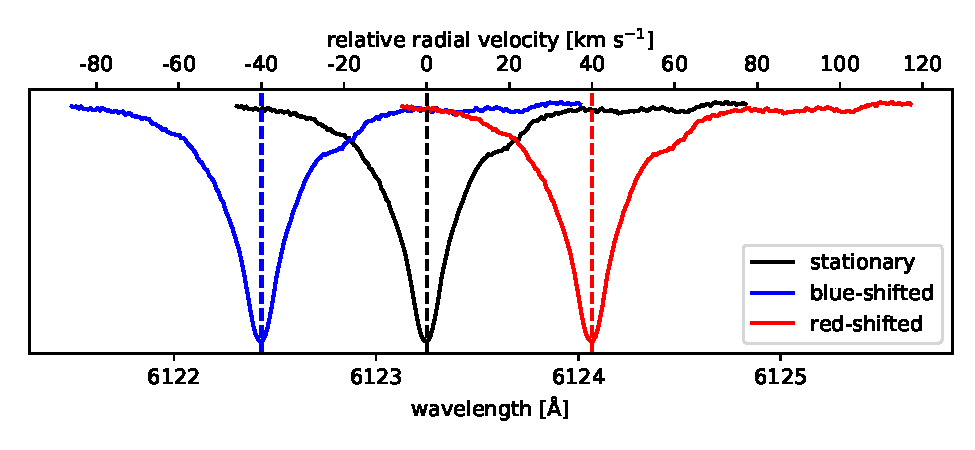
\includegraphics{figures-1/absorption-lines.pdf}
    \caption{Caption}
    \label{fig:absorption-lines}
\end{figure}

Measurement of the Doppler Effect, and therefore RVs, using spectroscopy leverages the existence of atomic absorption lines within the stellar spectra. As light travels from deep within the hot interior of the star (black body radiation that defines Wien's Law above), some of it is absorbed by the cooler and heavier gas in the outer layers of the star (or stellar atmosphere) resulting in less bright gaps across the spectrum. We know at which wavelengths these absorption lines should occur, due to studies in atomic physics and observations of our own Sun, and use them as points of comparison against the stellar spectra we collect with our spectrograph (see Figure \ref{fig:absorption-lines}). As the lines move further away in wavelength from where we expect them to be, the larger the measured RV.

A spectrograph's RV precision is therefore determined by how well it can measure the movement of these stellar absorption lines. There are two primary ways that this precision can be relayed \citep{fischer_state_2016}: (1) single-measurement precision or (2) long-term velocity scatter. The single-measurement precision states how well the instrument \textit{thinks} it can measure velocities. Resolution, bandwidth, typical measurement signal-to-noise ratio, and other instrument characteristics are all folded into this value, typically through statistical analysis while calculating the RV. Long-term velocity scatter, on the other hand, requires multiple RVs of the same target star. After a Keplerian model is fit to these RVs, the scatter is found by calculating average difference (or residual) between the model and the yielded RVs. This second metric is important to include since it may reveal systematic instrument issues unaccounted for in the single-measurement precision.

Finally, consideration needs to be made for the fact that, not only is the observed star moving due to pulls from possible exoplanets but, the Earth is hurtling through space around our own sun at nearly 30,000\ms, way faster than the RV semi-amplitude we are attempting to measure. Therefore, we must also employ a barycentric correction---modification of the wavelengths as if we had measured them from the stationary center of mass of our solar system---to our stellar spectra before making an RV measurement [CITATIONS]. Briefly, this is done by knowing two critical pieces of information: when ("What time?") and in which direction ("Where are you pointing the telescope?") the observation was made. Then, because the motion of Earth is quite well studied and therefore predictable, we can figure out the velocity the Earth is moving towards or away from the target star at the moment of observation and alter the wavelengths of the spectrum accordingly using Equation \ref{eq:relative-doppler-effect}.

\subsection{Limitations and Alternatives}

Unfortunately, there are some limitations in our ability to measure stellar spectra and these absorption lines consistently over time \citep{lovis_radial_2011}. The first is due to activity in the stellar atmosphere, which we collectively define as stellar noise. Whether it be through p-mode oscillations (large-scale pressure changes), granulation (small cells of convective motion), or cool spots and hot plages (dark and bright surface regions) that rotate with the star, stellar activity can mask itself as false RV signals on the order of 1--5\ms in the motion of the stellar absorption lines. In order to avoid this, users of the RV technique primarily study stars that they know are less noisy or, when possible, observe noisy stars long enough to average over the effects of stellar activity. Otherwise, a large portion of the field of RV spectroscopy is currently trying to find ways of disentangling the RVs from stellar noise from the RVs caused by planetary orbits [CITATIONS].

\begin{figure}
    \centering
    \includegraphics{figures-1/tellurics.pdf}
    \caption{Caption}
    \label{fig:tellurics}
\end{figure}

Another major limitation of the RV technique is caused by Earth's atmosphere, through what is called telluric contamination. After leaving the stellar atmosphere, light from the star travels only through the vacuum of space before finally reaching Earth. At this point, it must pass through an entire atmosphere before reaching the spectrograph, picking up new absorption lines from gases such as molecular oxygen and water vapor (see Figure \ref{fig:tellurics}). These telluric lines can overlap heavily with stellar absorption lines and, most importantly, they do not move with the radial velocity of the star. Rather, telluric lines need to be modeled and divided out (e.g. CITATIONS) or simply masked and avoided in RV measurement. Near-infrared spectrographs are hit hardest by telluric contamination due to the high opacity of the Earth's atmosphere (primarily water) in these wavelength regions.

Further limitations on RV measurement come from the instrumentation and spectrograph design. Throughput of light coupled from the telescope to the spectrograph is crucial to maximize. Less light from a single observation leads directly to lower RV precision, but we would prefer to not spend an entire night looking at a single target star to collect enough light for a measurable spectrum. However, this throughput tends to be inversely correlated with the resolution of the instrument, meaning careful consideration needs to be made to find a compromise between designed signal-to-noise and resolution \citep[e.g.][]{davis_insights_2017}. Also, consistency in the path of light as it travels through the spectrograph enables repeatable observations night after night. Factors such as temperature and pressure must be held constant to avoid altering the optical path and external vibrations must be absolutely mitigated to prevent flexures in the physical structure of the spectrograph optics. All told, the systematic effects of the instrument need to be significantly smaller than the amplitude of planetary signals, or otherwise carefully characterized, in order to have a chance at detection. This is especially true when trying to disentangle all three possible sources of motion: planets, stellar noise, and the instrument itself.

There have been numerous other methods of detecting and characterizing exoplanets, helping to fill out more possibilities of discovery as well as supplementing measurements made by the RV technique. In particular, the transit method---whereby a precision intensity-measuring instrument looks for exoplanets passing directly between its host star and the Earth, briefly dimming the stellar brightness---can provide information about exoplanet radii, enabling density approximations when combined with mass estimates from the RV technique \citep{fischer_exoplanet_2014}. The two major transit method satellite missions---Kepler \citep{borucki_kepler_2010}, along with its extension mission K2 \citep{howell_k2_2014}, and TESS \citep{ricker_transiting_2014}---are also providing thousands of exoplanet candidates with corresponding orbital periods, enabling better determination of observing strategies for the RV technique. Other exoplanet-detecting techniques include \citep{fischer_exoplanet_2014} direct imaging (measuring the light reflected off an exoplanet from its host star after blocking light from the star with a coronagraph), \textit{microlensing} (measuring the general relativistic bending of light due to the gravity of an exoplanet), and astrometry (measuring non-radial stellar positions over time).

\section{The State of the Field}

The history of the RV technique can be traced back through the various instruments used to make these measurements. As this is a publication on exoplanets and the RV technique, I feel compelled to include my own rendition of the exoplanet discovery data in Figure \ref{fig:rv-exoplanets} as it so clearly shows the progress made so far and the work we have ahead of us. From 1995 to 2010, there was steady improvement in RV measurement precision, with the minimum RV semi-amplitudes of discovered planets from 100\ms to 10\ms to 1\ms within this period. Over the past ten years, however, new discoveries have halted at about this 1\ms level, likely due to stellar activity being difficult to distinguish from planet-induced RVs at this instrumental precision. Therefore, as is evident by this dissertation, the role of those currently in RV instrumentation is to provide the tools necessary to break past this barrier.

\begin{figure}
    \centering
    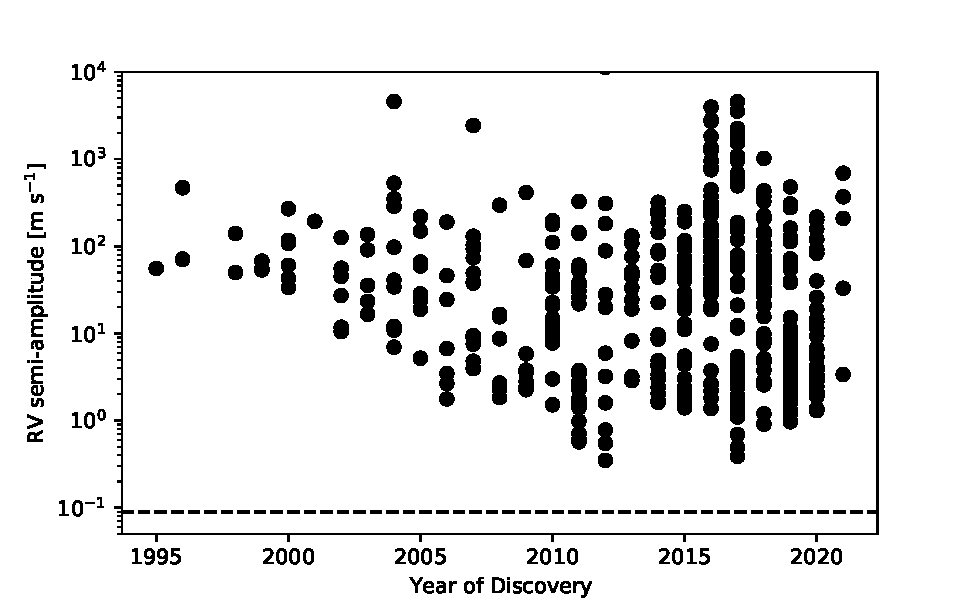
\includegraphics{figures-1/rv-exoplanets.pdf}
    \caption{Caption}
    \label{fig:rv-exoplanets}
\end{figure}

Table \ref{tab:spectrographs} lists just a handful of the many instruments---along with their designed resolution, bandwidth, and single-measurement RV precision---that have made measurement with the RV technique possible. More comprehensive lists can be found in \citet{fischer_state_2016} and \citet{wright_third_2017}. I have loosely grouped them into categories based on my own perceived ``eras'' of RV planet searches and briefly describe them here.

\begin{table}
    \centering
    \small
    \begin{tabular}{lcccc}
        \hline
        \hline
        Spectrograph & Year & Resolution & Bandwidth (nm) & SMP (\ms) \\
        \hline
        Hamilton & 1987 & 50,000 & 390-800 & 3.0 \\
        ELODIE & 1993 & 42,000 & 390--680 & 10.0 \\
        HIRES & 1996 & 55,000 & 364--800 & 3.0\rightarrow1.5 \\
        Tull & 1998 & 60,000 & 345--980 & 5.0 \\
        HRS & 2001 & 60,000 & 408--784 & 3.0 \\
        \hline
        HARPS & 2003 & 115,000 & 380--690 & 0.8 \\
        SOPHIE & 2006 & 75,000 & 387--694 & 1.1 \\
        PFS & 2010 & 76,000 & 390--670 & 1.2 \\
        CHIRON & 2011 & 90,000 & 440--650 & 1.0 \\
        HARPS-N & 2012 & 115,000 & 380--690 & 0.8 \\
        PARAS & 2012 & 67,000 & 380--690 & 1.0 \\
        APF+Levy & 2013 & 100,000 & 374--950 & 1.0 \\
        \hline
        MINERVA & 2016 & 75,000 & 480--690 & 0.9 \\
        CARMENES & 2016 & 90,000 & 520--1710 & 1.0 \\
        HPF & 2017 & 50,000 & 970--1810 & 1.0 \\
        MINERVA-Red & 2018 & & 820--920 & 1.0 \\
        ESPRESSO & 2018 & 134,000 & 380--780 & 0.1 \\
        EXPRES & 2018 & 137,500 & 380--840 & 0.3 \\
        MAROON-X & 2019 & 80,000 & 500--900 & 1.0 \\
        PARVI & 2019 & 100,000 & 1250--1800 & 0.3 \\
        iLocater & 2019 & $>$150,000 & 971--1270 & 0.7 \\
        NIRPS & 2019 & 100,000 & 970--1810 & $<$1.0 \\
        NEID & 2020 & 100,000 & 380--1000 & 0.3 \\
        KPF & 2021 & 85,000 & 440--850 & 0.3 \\
        G-CLEF & 2023 & 100,000 & 350--950 & 0.1 \\
        \hline
    \end{tabular}
    \caption{Past, current, and future RV spectrographs with tested or predicted metrics \citep{fischer_state_2016, wright_third_2017}.}
    \label{tab:spectrographs}
\end{table}

The detection of 51 Pegasi b was accomplished with the ELODIE spectrograph \citep{baranne_elodie_1996}, which actually had lower resolution and single-measurement precision than other astronomical spectrographs at the time. The Hamilton spectrograph \citep{vogt_lick_1987} at Lick Observatory, rather, had been searching for exoplanets since 1987 and was used to great effect, eventually with over 300 target stars \citep{fischer_planetary_1999}, until its decommissioning in 2011. The true work horse of this era (and even some to this day) is the HIRES spectrograph \citep{vogt_hires_1994} on the Keck Observatory 10~m telescope, observing more than 4000 target stars and steadily improving measurement precision through instrument upgrades up to 1.5\ms. Other spectrographs from this period include the High Resolution Spectrometer \citep{tull_high-resolution_1998} at the Hobby-Eberly Telescope and the Tull Spectrograph \citep{tull_high-resolution_1995} at McDonald Observatory.

Then, in 2003, the High-Accuracy Radial velocity Planetary Searcher spectrograph \citep[HARPS;][]{pepe_harps_2002, mayor_setting_2003} at the La Silla 3.6~m telescope in Chile set the new standard for RV spectroscopy. It was the first such instrument primarily designed to search for exoplanets and therefore included superior temperature, pressure, and vibration stability. This enabled an almost doubling of previous-generation resolution and an improvement to less than 1.0\ms precision, both significant achievements at the time. HARPS thus ushered in a wave of exoplanet discoveries, especially super-Earth- and Neptune-mass planets around solar-type stars \citep{pepe_harps_2011}, with over 2000 target stars. Over the next decade, older RV spectrographs began to be upgraded or replaced to meet this new standard: SOPHIE \citep{perruchot_sophie_2008} replaced ELODIE and the Automated Planet Finder (APF) with the Levy spectrograph \citep{vogt_apflick_2014} took the place of Hamilton. Also, a few new concept spectrographs came online, including CHIRON \citep{tokovinin_chironfiber_2013}, the PRL Advanced Radial-velocity Abu-sky Search spectrograph \citep[PARAS;][]{chakraborty_first_2010, chakraborty_prl_2014} and the Planet Finder Spectrograph \citep[PFS;][]{crane_carnegie_2006}. The success of HARPS also prompted a near copy to be built in the northern hemisphere, HARPS-N \citep{cosentino_harps-n_2014}, in 2012.

Now, we are in the age of the ``next-generation'' of RV spectroscopy with an explosion of new high-resolution spectrographs coming online in the last five years. This large diversity in investment with RV spectroscopy has enabled many new innovations to begin appearing. For example, many new spectrographs---such as CARMENES \citep{quirrenbach_carmenes_2016}, HPF \citep{mahadevan_habitable-zone_2014}, NIRPS \citep{wildi_nirps_2017}, and PARVI \citep{gibson_characterization_2020}---are beginning to explore the near-infrared, and therefore more M-type stars, to search for planets. Spectrographs like ESPRESSO \citep{pepe_espresso_2013}, EXPRES \citep{jurgenson_expres_2016} and NEID \citep{schwab_design_2016}, as well as future designs such as the Keck Planet Finder spectrograph \citep[KPF;][]{gibson_kpf_2016} and G-CLEF \citep{szentgyorgyi_gmt-consortium_2016}, on the other hand, are pushing the boundaries of visible-band spectroscopy through higher resolution, greater bandwidth, and extreme measures for environmental stability. We even have projects like iLOCATER \citep{crepp_ilocater_2016} that are trying to achieve both: extremely high resolution in the near-infrared. This truly is an exciting time to be an exoplanet hunter with the RV technique as there are simply so many avenues for possibility.

\section{The EXtreme PREcision Spectrograph} \label{intro:expres}

Nearly all of the work presented in this thesis was completed in support of the EXtreme PREcision Spectrograph \citep[EXPRES;][]{jurgenson_expres_2016, blackman_performance_2020, petersburg_extreme-precision_2020}, a high-resolution RV spectrograph commissioned at the Lowell Discovery Telescope outside Happy Jack, Arizona, in 2018. EXPRES was built as part of the 100-Earths project [CITATION], a collaboration between the Yale University Exoplanet Group and Lowell Observatory, with the express goal of finding 100 Earth-like planets within the next decade. Considering this requires RV measurement at the 0.1\ms level, the designing, commissioning, and maintenance of EXPRES has been a scientific and engineering feat since it was first conceived in 2014. This has involved everything from advanced optical fiber and laser technology, to precisely tuned environmental stability systems, to the development and implementation of new software to analyze data.

Therefore, in this section, I will be using EXPRES as a guide to introduce the physical and virtual mechanisms required make such precise measurements as the 0.1\ms wobble of a star. Naturally, the design decisions that went into EXPRES were built upon the strong pedigree of the RV community introduced in the previous section. Some of our decisions may differ from those of our contemporaries, but I try to address concerns as I have seen them. In the case of EXPRES, instrument design for RV spectroscopy can be split into four critical areas: (1) the optical fiber infrastructure, (2) the \'echelle spectrograph, (3) wavelength calibration sources, and (4) data extraction software. I introduce these areas here to motivate the work completed in this thesis.

\subsection{Optical Fiber Infrastructure} \label{intro:optics:fiber}

The first consideration for an RV spectrograph is determining how to couple light from a telescope into the instrument. Traditionally, instruments are attached right at a focus of the telescope, as is the case with many early RV spectrographs including HIRES, HRS, and Hamilton. However, considering the telescope moves constantly throughout the night to track target stars and is typically exposed to outside air temperature changes, this can cause problems with vibrational and thermal stability.

Instead, many RV spectrographs, including EXPRES, are coupled via optical fiber to the telescope. Optical fibers are long (meters to kilometers) thin (micrometers) tubes of glass that are able to transmit light from one end to the other, typically with high throughput. In principle, optical fibers propagate light due to a difference in the refractive index---a property ($n$) that determines the speed light moves through the material ($v=c/n$)---of the two concentric glass cylinders that make up the length of the fiber: the inner core and the outer cladding. When light enters the core at an angle and reaches the surface boundary at the cladding, rather than being transmitted into the cladding, the light reflects off the surface and continues traveling down the core, effectively bouncing its way from one end of the fiber to the other. This enables a great deal of flexibility in moving light from one place to another, since optical fibers can be bent around corners and precisely attached to other optical systems at either end.

Therefore, the use of optical fibers provides a great boon to RV spectroscopy. The spectrograph can be placed in a separate, possibly temperature-controlled and vibrationally-isolated, room near to the telescope (rather than on the telescope itself) with little loss to throughput. Optical fibers also provide spatial scrambling to stellar light, meaning input variations of the light---such as poor telescope guiding or changes in atmospheric density---are mitigated before illumination of the spectrograph optics \citep{hunter_scrambling_1992}. This effect can also be amplified through the use of double scramblers \citep{halverson_efficient_2015, spronck_fiber_2015} and non-circular fiber cross-sections \citep{chazelas_new_2010, spronck_use_2012, plavchan_precision_2013}. Finally, optical fibers enable many possibilities for alternative light sources, beyond the telescope, to enter the spectrograph. In the case of EXPRES, this involves an entire ``fiber architecture'' that includes multiple wavelength calibration sources (see Section \ref{intro:wvln_cal}), a flat-field calibration source (through two different sizes of fiber), and even an entirely different telescope that observes the Sun \citep{blackman_performance_2020}.

\begin{figure}
    \centering
    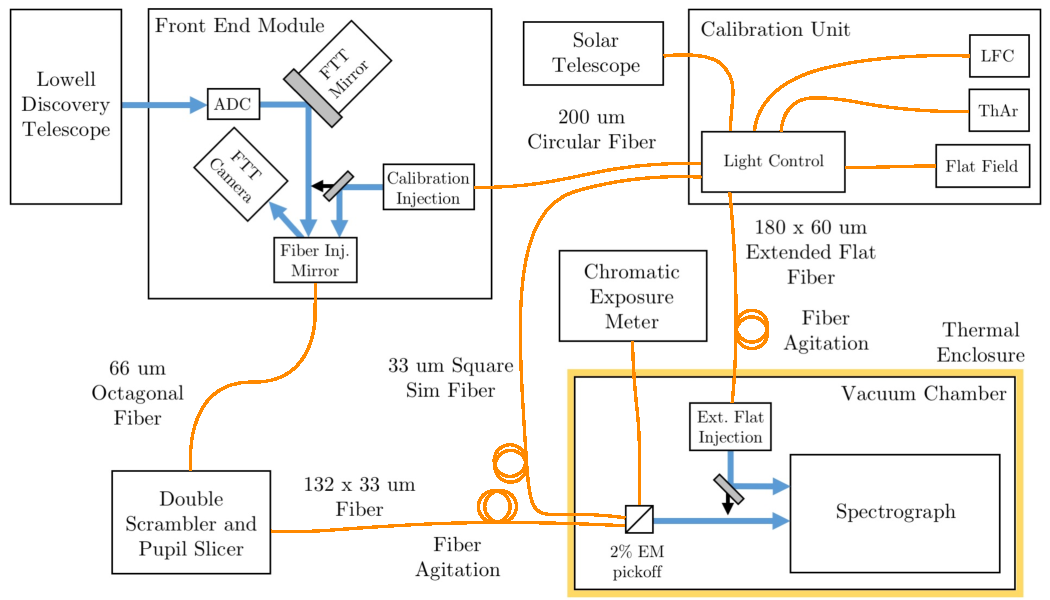
\includegraphics[width=\textwidth]{figures-1/expres_schematic_fibersV3.pdf}
    \caption{The EXPRES fiber architecture, reprinted from \citet{blackman_performance_2020}.}
    \label{fig:expres-fibers}
\end{figure}

There are, however, a few downsides to the use of optical fibers. To understand them, I will first introduce the ideas of focal ratio and numerical aperture. Light diverging from or converging to a single focus (such as is done by the cornea onto the retina of the human eye) does so in the shape of a cone, where the focus sits at the tip and the focusing optic (lens or mirror) sits at the base. The focal ratio (or $f/\#$) is the ratio between the height of this cone and the diameter of the base; a ``fatter'' cone means a lower focal ratio. The numerical aperture of an optical fiber---determined by the relative indices of refraction between the core and cladding ($\mathrm{NA}=\sqrt{n_{core}^2-n_{clad}^2}$)---then defines the minimum focal ratio accepted by the input ($f/\#_{min} \approx \frac{1}{2\mathrm{NA}}$). If light enters the fiber core at too steep an angle, it will not reflect off the cladding but rather dissipate out of the fiber.

Most optical fibers exhibit some form of focal ratio degradation (FRD), where light injected at a certain focal ratio is then output at a slightly lower focal ratio closer to the numerical aperture. FRD is exacerbated by tight bends and especially cracks in the fiber \citep{ramsey_focal_1988}. This means the focal ratio of the telescope should not exceed the numerical aperture of the optical fiber and the fibers need to be vetted and characterized for FRD to understand how the cone of light will change before entering the spectrograph. The spectrograph subsequently needs to be designed such that it will accept as much of the output cone of light as possible. The other major issue with optical fibers, modal noise, is more comprehensively introduced and rectified in Chapter \ref{chapter:modal-noise}.

\subsection{\'Echelle Spectroscopy} \label{intro:optics:echelle}

\begin{figure}
    \centering
    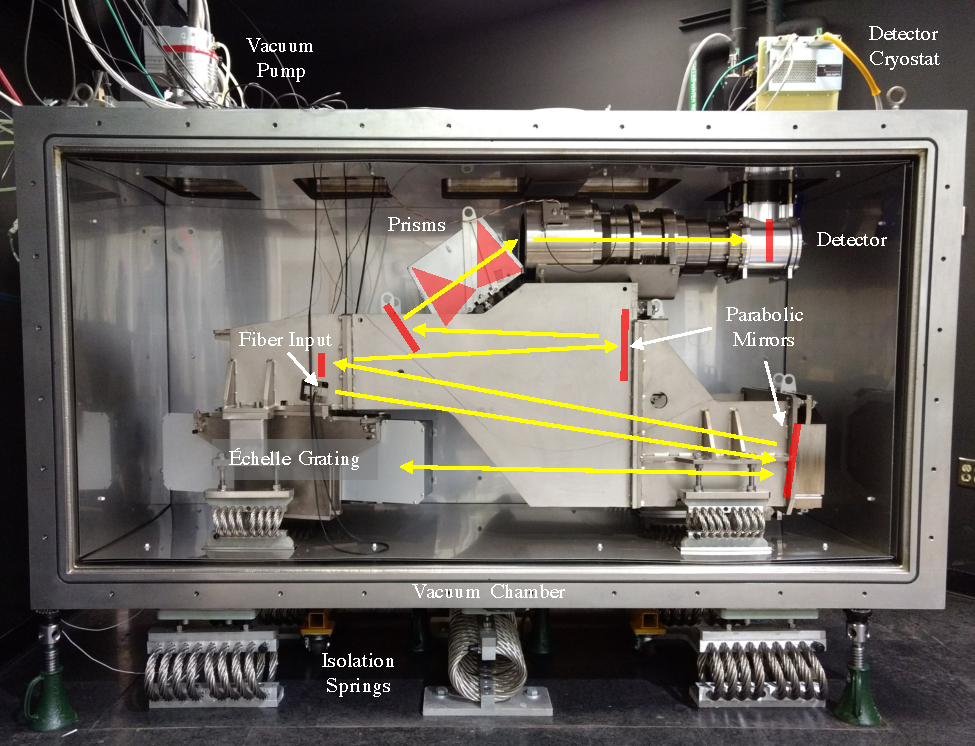
\includegraphics{figures-1/expres.pdf}
    \caption{A real image of the EXPRES \'echelle spectrograph with an overlayed optical path and labels for the various optical components.}
    \label{fig:expres}
\end{figure}

Once light is coupled from the telescope, nearly all RV spectrographs follow a similar optical path to the one shown in Figure \ref{fig:expres} for EXPRES. In particular, this type of instrument is known as an \'echelle spectrograph. Diverging light from the input is collimated---made cylindrical, like light from a laser pointer---by a parabolic mirror towards the \'echelle grating. An \'echelle grating serves a similar function to the prism in my example before, separating the light into its various constituent wavelengths spatially, however, not with a single continuous spectrum. Rather, an \'echelle grating exploits the diffraction equation
\begin{equation}
    d \sin{\theta} = m \lambda
    \label{eq:diffraction}
\end{equation}
to reflect multiple shorter spectra that happen to be spatially overlayed with each other. Consider two separate sets of grating orders ($m$) and wavelengths: ($m_1=100$, $\lambda_1=500~\mathrm{nm}$) and ($m_2=150$, $\lambda_2=400~\mathrm{nm}$). Each of these pairs yield the same $d\sin{\lambda}$ meaning they are reflected at the exact same angle by the \'echelle grating! Or, simply, $m_1\lambda_1 = m_2\lambda_2$. Specifically, the EXPRES \'echelle grating is designed to maximally reflect horizontally overlapping segments of orders 84 to 160 right back at the first collimating mirror.

After leaving the \'echelle grating, the light is then focused near a small optical correcting mangin mirror, which subsequently reflects the light back to another parabolic mirror. The collimated light is then reflected again using a simple flat mirror through a pair of cross-dispersing prisms. These prisms vertically separate the overlapping orders produced by the \'echelle grating, enabling us to differentiate between them spatially. These prisms are known as ``cross-dispersing'' because they diffract the light perpendicularly to the ``dispersion'' done by the \'echelle grating. After traveling through the prisms, the light is finally focused onto the spectrograph's detector, yielding the image shown in Figure \ref{fig:expres-format}. Just like the orientation of EXPRES, the horizontal dimension of this image is known as the dispersion-direction and the vertical dimension is known as the cross-dispersion direction.

\begin{figure}
    \centering
    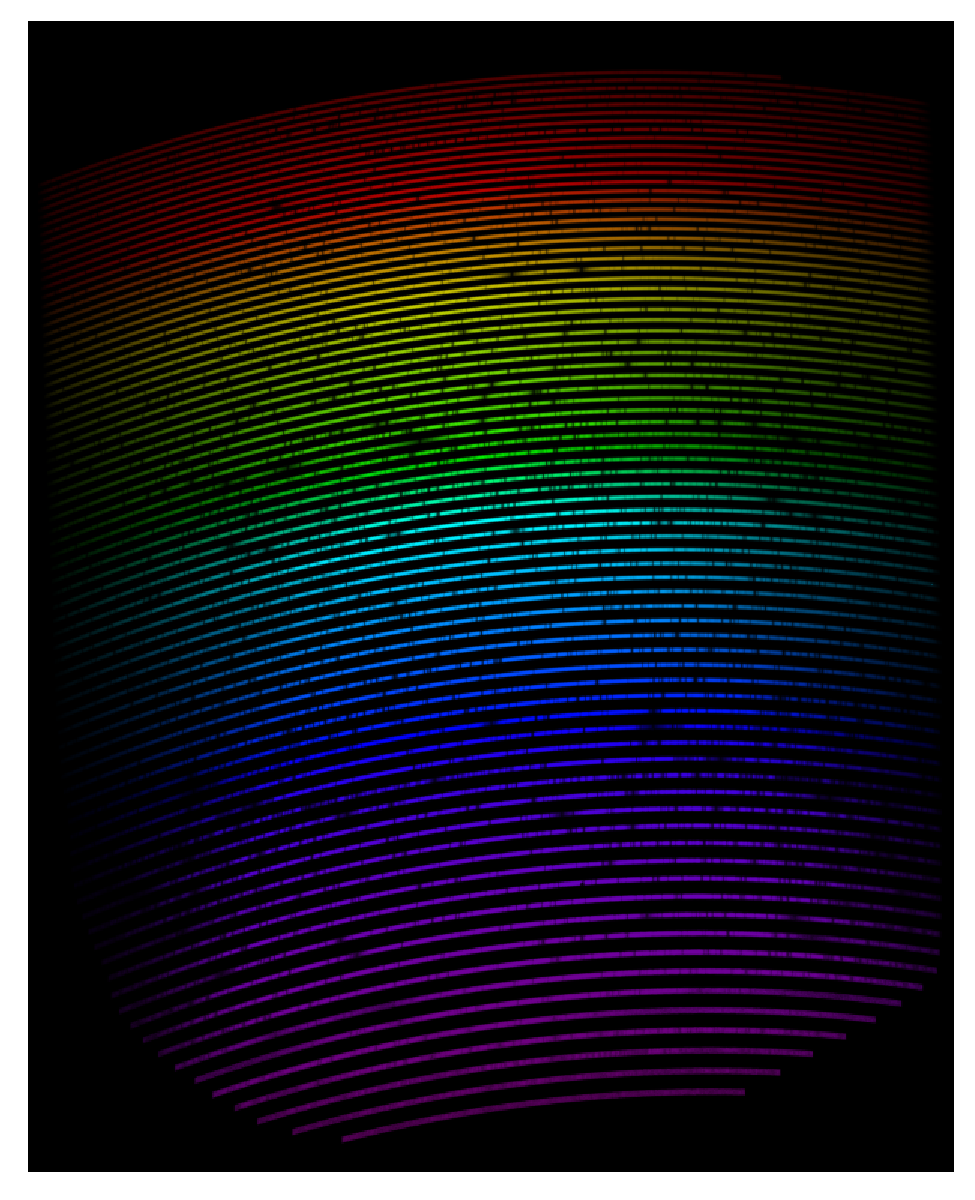
\includegraphics{figures-1/expres-format.pdf}
    \caption{Caption}
    \label{fig:expres-format}
\end{figure}

The EXPRES detector is a Charge-Coupled Device (CCD) that converts photons---``particles'' of light---into electrons within a large number of discrete pixels arranged as a two-dimensional array. The efficiency with which each pixel can make this conversion is called its quantum efficiency (QE). The CCD, after a set exposure time, then transfers and amplifies these electrons through a series of read-out electronics to convert them into a digital signal for processing by a computer. The conversion ratio between this digital value and the true number of counted electrons is called the gain. There are two important sources of noise during this process: photon noise and read noise. Photon noise is caused by the quantized nature of light; only an integer number of photons can hit any given pixel. Therefore, random fluctuations in brightness are predicted by Poisson statistics: the expected standard deviation of $N$ photons hitting a given pixel is $\sigma_\gamma=\sqrt{N}$. Read noise is rather an inherent property of each CCD pixel. As the photon-induced electrons (or photo-electrons) are read out, there is some scatter to the read values, whose standard deviation is defined as $\sigma_r$. These two terms are typically added in quadrature ($\sigma=\sqrt{\sigma_\gamma^2 + \sigma_r^2}$) to yield the a complete noise model for each CCD pixel. Ideally, CCDs are developed with maximum QE and minimum $\sigma_r$.

Figure \ref{fig:expres} also reveals some of the environmental stability measures taken by EXPRES \citep{jurgenson_expres_2016}. The entire optical bench is built within a large vacuum chamber (meaning we are normally not able to see it) to maintain an extremely low and stable pressure ($1\times 10^{-7} \pm 2\times 10^{-8}$~torr) as well as less than $0.075$~K per day drifts in temperature\citep{blackman_performance_2020}. The optical bench itself is also constructed from Invar, a nickel-iron alloy that flexes very little at changing temperatures. Along the bottom are also two sets of springs that vibrationally isolate the spectrograph from the slab it is sitting on, which itself is physically isolated from the rest of the telescope building foundation.

\subsection{Wavelength Calibration} \label{intro:wvln_cal}

In order to extract stellar spectra, RV spectrographs use the spectra of well-characterized and stable light sources as a simultaneous or observation-bracketing reference on the spectrograph camera. These can be thought of as the ``rulers'' or ``yardsticks'' of RV measurement. Historically, thorium argon (Th-Ar) lamps and iodine reference cells have been used to calibrate RV spectrographs since their spectral properties are well understood and their bandwidth covers most of the visible spectrum. However, both of these light sources have inherent issues that limit RV measurements to approximately \SI{1}{\meter\per\second} precision. Th-Ar emission lines are broad, saturated, and irregularly spaced, meaning some wavelength regions are less well calibrated than others. The iodine technique, which applies absorption wavelengths directly on the stellar spectrum, masks the subtle spectral line profile effects imprinted by stellar activity. Furthermore, iodine introduces complexity, such as parameter cross talk, to the forward modeling \citep{spronck_fiber_2015} and the cells themselves may not have long term mechanical stability \citep{fischer_twenty-five_2014}.

More recently, RV spectrographs have employed frequency combs (FCs), synthesized spectra containing sharp peaks of intensity at equally spaced frequencies, with the intention of better stability and therefore precision in their wavelength calibration. Ideally, the lines of a FC are non-overlapping and located at precisely determined wavelengths with flat intensity, to avoid over- or under-saturating pixels on the spectrograph detector. The FC must also have the proper free spectral range (FSR, frequency separation of comb lines) across the entire bandwidth of the spectrograph optics so that the detector can resolve each peak (more than $\sim$\SI{10}{\giga\hertz}) and calibrate a sufficient number of stellar frequencies (less than $\sim$\SI{40}{\giga\hertz}). Also, the zero-point frequency offset ($f_0$) and FSR should not drift over both short (seconds) and long (months) time scales. Most FC devices have been developed for the near-infrared, due to the proliferation of telecom interest around \SI{1550}{\nano\meter}, and this has been sufficient for observing M dwarf exoplanets \citep{fischer_state_2016}. However, to address planetary system statistics for late F, G, and early K type stars, the wavelength range will need to stretch through the visible to better calibrate many more absorption lines. It is especially important to reach the Calcium H \& K lines located below \SI{400}{\nano\meter} that contain chromospheric activity information that characterizes photospheric noise \citep{isaacson_chromospheric_2010, lovis_harps_2011}.

A relatively cheap way to produce a broadband optical FC is using a tunable Fabry-P\'erot (FP), a resonant cavity that employs feedback to correct for drifts in length. They do not offer an inherent $f_0$ calibration, however, and must be referenced against a separate stable source for bootstrapped calibration \citep{mccracken_single-lock_2014, sturmer_rubidium-traced_2018} meaning the system cannot be self-contained. Therefore, fixed-length FP etalons were developed to mitigate this issue. However, \citet{reiners_laser-lock_2014} and \citet{wildi_passive_2012} have shown that the set distance between the two reflective surfaces still drifts unpredictably, especially over long time scales, thereby continuing to limit spectrograph precision to only $\sim$\SI{1}{\meter\per\second}.

Menlo Systems has built perhaps the most advanced wavelength calibrator for visible RV spectroscopy, a laser FC that reaches $\sim$\SI{1}{\centi\meter\per\second} RV precision \citep{probst_laser_2014}. This FC pulses a femtosecond mode-locked laser to produce high finesse lines and an extremely stable FSR. Unfortunately, these lines are too tightly spaced for RV spectrographs, therefore the system must use line-by-line spectral filtering with multiple tunable FP cavities to suppress most of the produced frequencies. There are consequently some critical limitations to this device: complexity, cost, and limited bandwidth. The Menlo FC requires a continuing service contract to properly maintain it and thus has not yet reach true ``turn-key'' status. Also, this technology costs approximately \$1,000,000---a prohibitive price point for smaller RV projects---and is extremely bulky, limiting its use to larger ground-based spectrographs. Furthermore, the system is still limited to $\sim$\SI{450}{\nano\meter} thereby excluding the critical Calcium H \& K lines below \SI{400}{\nano\meter}.

A promising and growing field of astro-comb development includes electro-optic modulation (EOM) combs and chip-based waveguide technologies [CITATIONS OUT THE WAZOO]. These devices offer ease-of-use along with a much more affordable price point, since EOM combs can be built using primarily off-the-shelf components while waveguides can be fabricated and tuned in-house to meet the needs of the instrument. These technologies are the focus of my work in Chapter \ref{chapter:astro-comb}, therefore, I provide further introduction to them there.

Emission line wavelength calibration sources have another important function for the instrument: point spread function characterization. Since an \'echelle spectrograph converts spectral information into spatial information, a spectral point source (i.e. a single wavelength laser) would ideally be mapped as a physical point source on the spectrograph's detector. However, Within any optical re-imaging system, light is not perfectly translated from input to output. Rather, the light undergoes optical aberrations modifying it as it is reflected and diffracted throughout the system and, importantly, these effects are typically wavelength dependent. Therefore, shining a single wavelength laser into a spectrograph reveals exactly the optical aberrations, or point spread function, of the instrument at that wavelength. Emission line wavelength calibration sources are simply a collection of hundreds or thousands of such single wavelength lasers, thus they can be used to map the point spread function of a spectrograph across its entire spectral format, as I demonstrate in Chapters \ref{chapter:astro-comb} and \ref{chapter:spec-perf}.

EXPRES uses a Menlo LFC primed by a ThAr lamp to complete its nightly wavelength calibrations. The principles of this process are shown in Figure \ref{fig:calibration}. The wavelengths of ThAr emission lines are easily identifiable using data from previously collected ThAr atlases \citep{palmer_atlas_1983, redman_spectrum_2014}. These lines then provide a close guess for the wavelengths of some LFC lines which can subsequently all be identified using the LFC's known FSR and $f_0$. These wavelengths are then interpolated to match the grid of spectral bins of the provided spectrum. Further specifications for this process can be found in Chapter \ref{chapter:pipeline}.

\begin{figure}
    \centering
    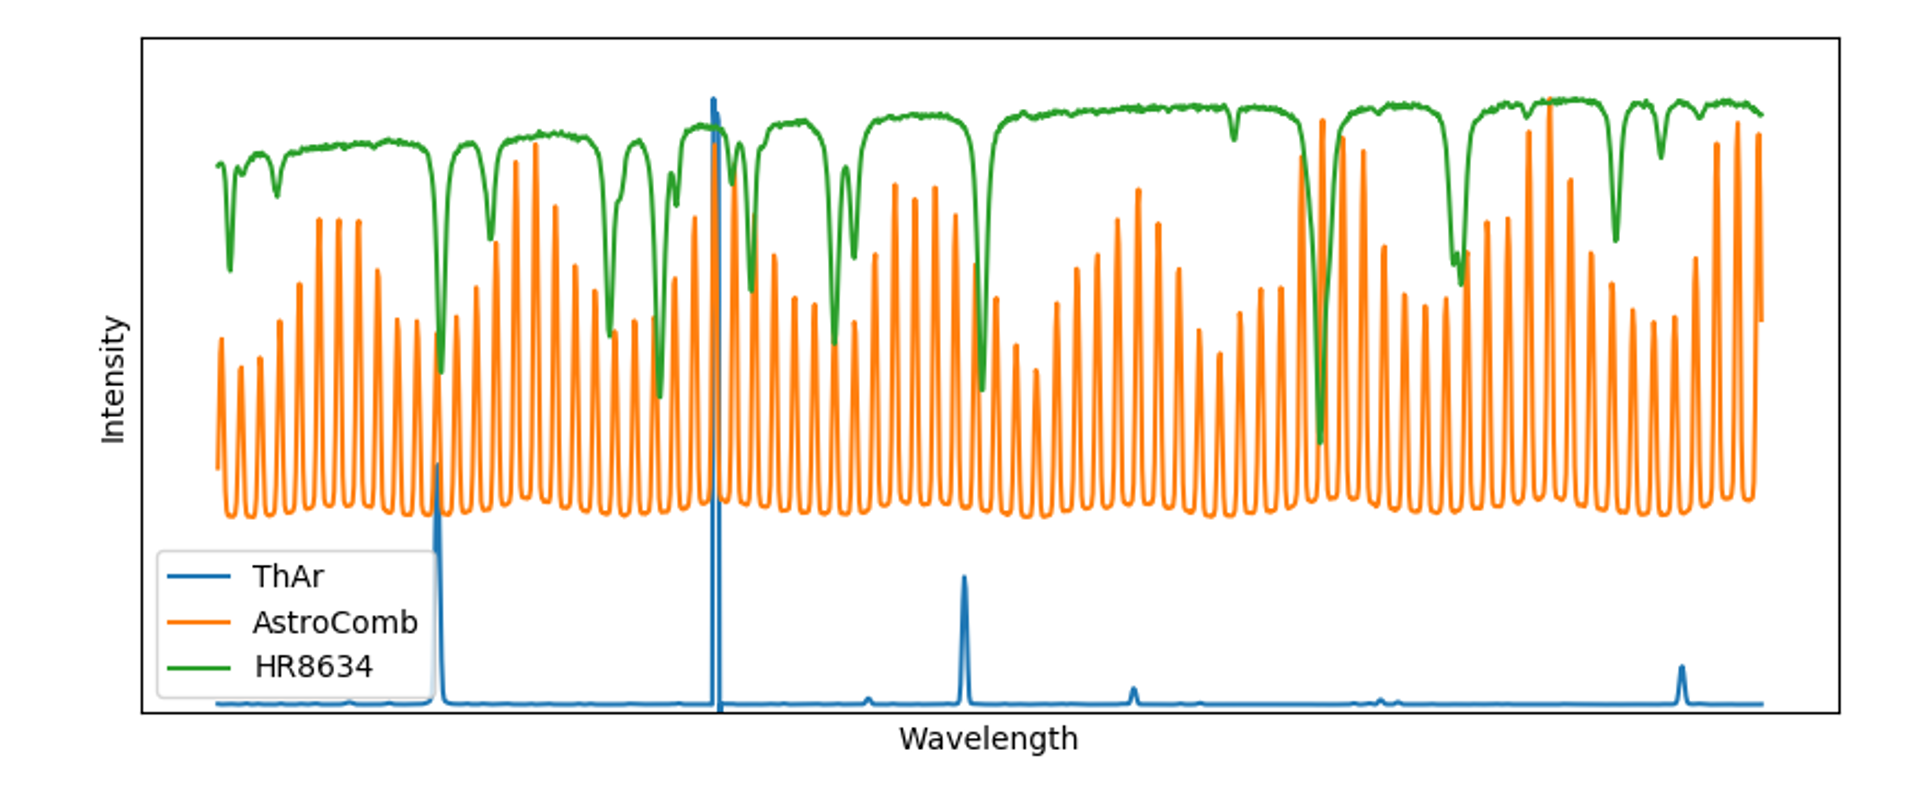
\includegraphics{figures-1/calibration.pdf}
    \caption{Three stages of wavelength calibration for EXPRES. ThAr lines are used as a primer for the LFC lines which are finally used to generate wavelengths for the spectrum.}
    \label{fig:calibration}
\end{figure}

Finally, consideration needs to be made as to \textit{when} wavelength calibrations are made as part of the observation strategy. Namely, the decision between simultaneous calibrations---measuring the wavelength calibrator at the same time as the star except through a separate fiber---and bracketed calibrations---using the same fiber but alternating between stellar and calibration observations. Simultaneous calibrations have two inherent downsides: (1) a requirement to tailor the brightness of the calibrating light source to match signal-to-noise over various length of science observations (i.e. brighter and dimmer stars) and (2) systematic changes in the optical system may not perfectly correlate between separate fibers, meaning extra analysis is necessary to translate wavelength solutions generated by the simultaneous calibration light path to the science light path. Therefore, EXPRES uses bracketed calibrations in order to more consistently control the brightness of its laser frequency comb (which can reach a sufficient signal-to-noise level within only 10 seconds) and to calibrate the instrument using the same optical path and detector pixels as science observations.
% As demonstrated in Chapter \ref{chapter:pipeline}, various methods of interpolation are more than sufficient to then project these bracketed wavelength solutions to midpoint time of intermediate observations.

\subsection{Data Extraction} \label{intro:extraction}

The final step of completing an RV spectrograph is in developing code for data extraction: taking raw pixel data from the instrument's detector, converting it into a wavelength-calibrated barycentric-corrected spectrum, and using it to calculate the RV of the given observation. Unfortunately, the raw data of EXPRES is not as nice as in Figure \ref{fig:expres-format}, but rather it looks like Figure \ref{fig:expres-raw}. The CCD is split into 16 distinct regions which each have their own overscan regions (virtual pixels that reveal fundamental properties of the read-out electronics) and gain. The first step of extraction, which I call ``reduction'', involves combining these separate regions while correcting (QE, gain, dark counts, bias) or characterizing (photon noise, read noise) inherent properties of the data.

\begin{figure}
    \centering
    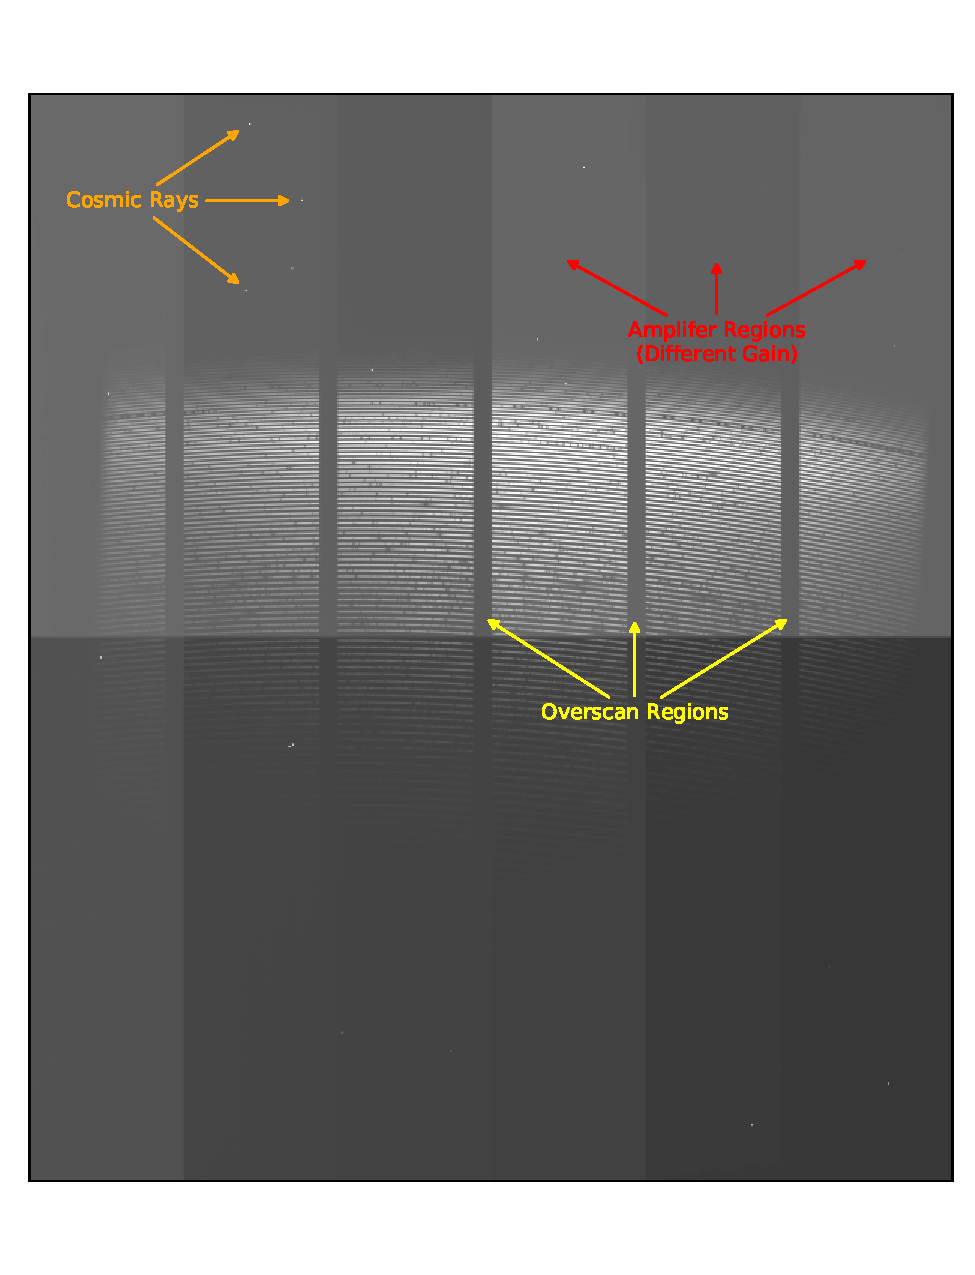
\includegraphics{figures-1/expres-raw.pdf}
    \caption{Caption}
    \label{fig:expres-raw}
\end{figure}

After reduction, the two-dimensional data contained within the 86 separate \'echelle orders can now be converted into a one-dimensional spectrum. Historically, there have been three methods of spectral extraction developed for RV spectrographs. Boxcar extraction involves simply summing up counts column-by-column along each order. Optimal extraction takes this a step further by developing an expected model for the cross-sectional shape of each order and fitting only a scaling factor to each column, enabling improved signal-to-noise performance and cosmic-ray rejection \citep{horne_optimal_1986}. Finally, spectro-perfectionism has provided a framework for expanding this model into a second dimension, enabling maximum information transfer from CCD to spectrum \citep{bolton_spectro-perfectionism_2009}. Further exploration of optimal extraction and spectro-perfectionism are provided in Chapters \ref{chapter:pipeline} and \ref{chapter:pipeline2} respectively. Introductions to methods for wavelength calibration, barycentric correction, and telluric modeling are also all provided in Chapter \ref{chapter:pipeline}.

Finally, we reach the stage of calculating the RV for each stellar observation. Cross-correlation \citep{baranne_coravel_1979}, taking a delta-function model of the known stellar lines and convolving this against the spectrum to find a maximum overlap point, has been extremely popular and successful at measuring RVs for a wide variety of instruments \citep[e.g.][]{freudling_automated_2013, brahm_ceres_2017, modigliani_espresso_2019}. More recently, however, further exploration has gone into forward modeling techniques---using generated templates of stellar spectra as models for least-squares fitting of an offset velocity \citep[e.g.][]{zechmeister_spectrum_2018, rajpaul_robust_2020}. An important part of either of these processes lies in the identification of stellar activity indicators within the spectrum \citep[e.g.][]{davis_insights_2017, dumusque_measuring_2018}, in order to avoid/mitigate potentially problematic stellar lines or to provide a systematically-corrected offset to the calculated RV.

\section{Thesis Outline} \label{intro:structure}

In this thesis, I present the design and implementation of multiple novel methods---within instrumentation and data extraction---that have shown demonstrable improvement to many of the aspects of fiber-fed radial velocity spectroscopy outlined in the previous section. The thesis is split into four chapters. Chapter \ref{chapter:modal-noise} describes my investigation into the inherent properties of optical fiber modal noise and my conclusions about how best to mitigate this potentially devastating noise source. Chapter \ref{chapter:astro-comb} details my explorations into the use of Aluminum Nitride as an on-chip waveguide material to support RV spectroscopy, both through validation of blue-wavelength throughput using a micro-comb design and my foray into the design of a 16~GHz EOM comb as a possible next-generation precision visible-wavelength astro-comb. Chapter \ref{chapter:pipeline} outlines the EXPRES data extraction pipeline, through which I implemented numerous novel algorithms, resulting in a single measurement precision of 0.3\ms for the instrument. Chapter \ref{chapter:pipeline2} demonstrates my additional contributions to the EXPRES pipeline, beyond the defaults described in Chapter \ref{chapter:pipeline}, including spectro-perfectionism and the use of \textit{B}-spline regression to generate stellar templates. Finally, Chapter \ref{chapter:conclusion} provides a summary of my findings as well as my personal lessons learned from my instrumentation experience and a list of recommended future work that could expand upon the research in this thesis. Chapters \ref{chapter:modal-noise} and \ref{chapter:pipeline} are adapted from peer-reviewed journal articles with a few added updates since their publication, while Chapters \ref{chapter:astro-comb} and \ref{chapter:pipeline2} are both completely new material.
	\chapter{Modal Noise Mitigation through Fiber Agitation for Fiber-fed Radial Velocity Spectrographs}\label{chapter:modal-noise}

\begin{center}
    Adapted from

    \textit{Ryan R. Petersburg, Tyler M. McCracken, Dominic Eggerman, Colby A. Jurgenson, David Sawyer, Andrew E. Szymkowiak, and Debra A. Fischer}
    
    The Astrophysical Journal, Volume 853, Number 2, Page 181, 2018
\end{center}

\section*{Abstract}

Optical fiber modal noise is a limiting factor for high precision spectroscopy signal-to-noise in the near-infrared and visible. Unabated, especially when using highly coherent light sources for wavelength calibration, modal noise can induce radial velocity (RV) errors that hinder the discovery of low-mass (and potentially Earth-like) planets. Previous research in this field has found sufficient modal noise mitigation through the use of an integrating sphere, but this requires extremely bright light sources, a luxury not necessarily afforded by the next generation of high-resolution optical spectrographs. Otherwise, mechanical agitation, which ``mixes'' the fiber's modal patterns and allows the noise to be averaged over minutes-long exposures, provides some noise reduction but the exact mechanism behind improvement in signal-to-noise and RV drift has not been fully explored or optimized by the community. Therefore, we have filled out the parameter space of modal noise agitation techniques in order to better understand agitation's contribution to mitigating modal noise and to discover a better method for agitating fibers. We find that modal noise is best suppressed by the quasi-chaotic motion of two high-amplitude agitators oscillating with varying phase for fibers with large core diameters and low azimuthal symmetry. This work has subsequently influenced the design of a fiber agitator, to be installed with the EXtreme PREcision Spectrograph, that we estimate will reduce modal-noise-induced RV error to less than \SI{3.2}{\centi\meter\per\second}.


\section{Introduction}
\label{modal-noise:intro}

Radial velocity (RV) exoplanet detection has continuously been on the path toward higher precision to enable the detection of less massive and longer period planets. The current goal of RV spectroscopy is \SI{10}{\centi\meter\per\second} precision, a factor of 10 better than current state-of-the-art RV spectroscopy, thereby allowing the discovery of Earth-like planets orbiting G and K stars in their respective habitable zones \citep{fischer_state_2016}. The next-generation of visible-band RV spectrographs---including but not limited to the EXtreme PREcision Spectrograph (EXPRES; \citet{jurgenson_expres_2016}), ESPRESSO \citep{megevand_espresso_2012}, NEID \citep{schwab_design_2016}, and the Keck Planet Finder \citep{gibson_kpf_2016}---require precision engineering and extreme stability to reach this goal.

Fiber coupling the spectrograph to the telescope has become an essential and standard method for planet hunting spectrographs. Separating the spectrograph from the telescope by a fiber tens of meters long enables the spectrograph to be located in a controlled environment, isolating it from vibrational and thermal noise. Linking the telescope to the spectrograph via fiber also leverages the spatial scrambling properties inherent to fibers that, for the most part, decouple input variations from the output producing a stable illumination of the spectrograph optics \citep{hunter_scrambling_1992}. This effect has been amplified through the use of double scramblers \citep{halverson_efficient_2015, spronck_fiber_2015} and non-circular fiber geometries \citep{chazelas_new_2010, spronck_use_2012, plavchan_precision_2013}.

Optical fibers also transmit light from calibration sources, such as wavelength calibrators and broadband flat-field sources, to the spectrograph. Laser frequency combs, especially the  astrocomb \citep{probst_laser_2014} recently deployed at HARPS and soon at EXPRES, produce thousands of ultra-narrow, evenly spaced emission lines over a wide frequency range. When these highly coherent lines propagate through a multi-mode fiber, they create a source of noise that limits the signal-to-noise ratio (S/N) of the instrument and potentially induces false RV signals in the data. This noise is caused by interference between the finite number of electromagnetic modes that can propagate along a multi-mode fiber, and therefore the term \textit{modal noise} has been coined for this effect \citep{epworth_phenomenon_1978}.

Some next-generation RV spectrographs---e.g. iLocater \citep{crepp_ilocater_2016} and MIN\-ERVA-red \citep{blake_minerva-red_2015}---have moved to a completely single-mode fiber architecture to help alleviate these complications. As apparent in their name, single-mode fibers only propagate a single spatial mode and should be free from any modal noise. Due to the small core size of single-mode fibers, however, coupling light from the telescope into these fibers is challenging and requires robust adaptive optics not currently available in the visible. Single-mode fibers also have a limited bandwidth---approximately 100--\SI{200}{\nano\meter} in the visible and 400--\SI{600}{\nano\meter} in the near infrared---over which they propagate a single mode. Thus, the fiber architectures for these spectrographs require multiple band-dependent paths or endlessly single-mode photonic crystal fibers (yet untested in RV spectroscopy) for broadband coverage. It is also possible that single-mode fibers are not free from modal noise since they propagate in two polarization modes that have been shown to affect spectrograph performance \citep{halverson_modal_2015}. The study of modal noise reduction methods may still be necessary even regarding the existence of these novel single-mode fiber-fed instruments.

In this paper, we attempt to discern the optimal strategy for reducing modal noise using mechanical agitation on multi-mode fibers propagating coherent visible light. We begin by defining modal noise and exploring how previous experiments have mitigated it through static and dynamic methods (Section \ref{modal-noise:mn}). We then describe our own methods of fiber agitation (Section \ref{modal-noise:exp-setup}) and discuss results from using these methods on fibers of varying cross-sectional shapes and coupling permutations (Section \ref{modal-noise:results}). Finally, we relate these results to limits in RV precision (Section \ref{modal-noise:rv-precision}), test how our agitation methods affect focal ratio degradation (FRD; Section {\ref{modal-noise:frd}}), and discuss how these results should be applied to next-generation RV spectrographs (Section \ref{modal-noise:conclusions}). The work in this paper was conducted to influence design decisions for EXPRES.

\section{Optical Fiber Modal Noise}
\label{modal-noise:mn}

Light propagates through an optical fiber in an integer number of electromagnetic modes. The exact calculation for this value is nontrivial since it depends on the instantaneous fiber geometry, injection parameters, and many other variables. The maximum number of modes for a step-index circular cross-section fiber (propagating a relatively large number of modes) with a monochromatic light source is approximately
\begin{equation}
M_{circ} \approx \frac{4}{\pi ^2} V^2 = \frac{4}{\pi ^2} \Bigg( \frac{2 \pi r \mathrm{NA}}{\lambda} \Bigg) ^2.
\label{eq:max_modes}
\end{equation}
$V$ is the normalized frequency of the fiber rewritten in terms of $\mathrm{NA} = \sqrt{n_\mathrm{core}^2 - n_\mathrm{clad}^2}$, the numerical aperture of the fiber determined by the core ($n_\mathrm{core}$) and cladding ($n_\mathrm{clad}$) indices of refraction, the core radius $r$, and the wavelength $\lambda$ of propagated light. This approximation is more difficult for a rectangular fiber, but \citet{nikitin_estimating_2011} shows empirically using electromagnetic and geometrical arguments that
\begin{equation}
\frac{M_\mathrm{rect}}{M_\mathrm{circ}} \approx 2 \frac{ab}{\pi r^2}
\label{eq:prop_modes}
\end{equation}
where $a$ and $b$ are the side lengths of the rectangular cross-section. Notice that $ab$ and $\pi r^2$ give the areas for a rectangle and circle respectively. From this, we will assert more generally, with some rearrangement of Equation (\ref{eq:max_modes}), that
\begin{equation}
M_{s} \approx \frac{16}{\pi} C_{s} A \Bigg( \frac{\mathrm{NA}}{\lambda} \Bigg) ^2
\label{eq:mode_area}
\end{equation}
where $A$ is the cross-sectional area of the fiber and $C_{s}$ is a constant coefficient dependent on fiber cross-sectional shape such that $C_\mathrm{circ} = 1$ and $C_\mathrm{rect} = 2$. $C_{s}$ is so far unknown for more complicated geometries, but we assume that $C_{s} \sim 1$.

\begin{figure}
\centering
	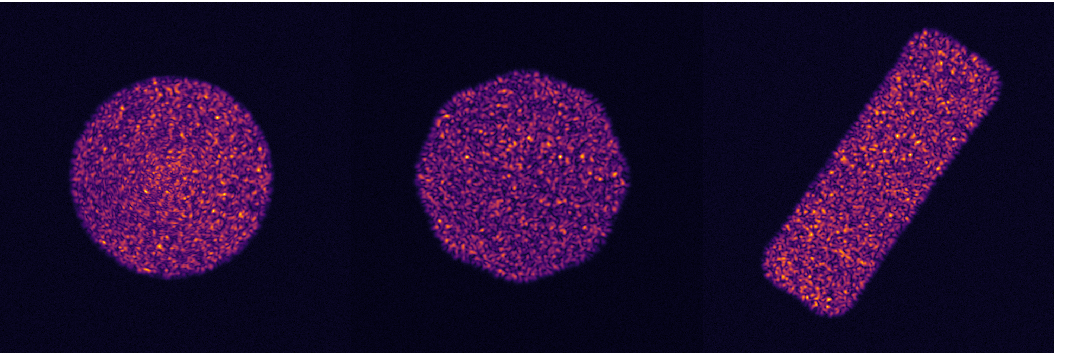
\includegraphics[width=\columnwidth]{figures-2/fiber_example.pdf}
	\caption[Fiber faces affected by modal noise]{Examples of unmitigated modal noise for a \SI{200}{\micro\meter} circular (left), \SI{200}{\micro\meter} octagonal (middle), and \SI{100x300}{\micro\meter} rectangular (right) optical fiber. All three fibers shown here have approximately the same cross-sectional area, meaning that they each are propagating about the same number of electromagnetic modes (see Equation (\ref{eq:mode_area})). Brightness in this image is scaled by (photon count)$^{0.6}$ for better presentation of the range of speckle brightness. The contrast of the speckles is therefore \textit{worse} than what is shown here.}
\label{fig:fiber_example}
\end{figure}

When coherent light is propagated through a multi-mode fiber, a high contrast speckle pattern known as modal noise is produced at the output for both the near field (fiber face projected onto a detector, Figure \ref{fig:fiber_example}) and far field. Modal noise is an inherent property of all multi-mode fibers regardless of the cross-sectional core shape \citep{sablowski_comparing_2016}. It arises from light coupling from mode-to-mode as it propagates through the fiber, causing slight variances in the path length traveled and producing the observed interference pattern. For RV spectrographs, this causes two problems: (1) it limits the maximum S/N and (2) systematic variations in the speckle pattern will mask themselves as minute shifts on the focal plane causing errant RV signatures.

\subsection{Limit on S/N}

Due to its high contrast, modal noise can severely decrease the S/N of an RV spectrograph \citep{epworth_phenomenon_1978, baudrand_modal_2001, lemke_modal_2011, iuzzolino_preliminary_2014}. For a fiber without spatial filtering or a slit, the magnitude of this noise is proportional to $\sqrt{M_s}$ \citep{goodman_statistics_1981}. Therefore, increasing the size of the fiber, increasing the numerical aperture of the fiber (or decreasing the injected focal ratio), and decreasing the wavelength of injected light should increase the S/N due to modal noise. It also appears that changing the fiber core shape could affect the S/N.

Experimental results of these conditions have been well documented. S/N due to modal noise has been shown empirically to
\begin{enumerate}
\item increase with larger fiber core cross-sectional area \citep{lemke_characterising_2010, sablowski_comparing_2016},
\item decrease with larger focal ratios \citep{baudrand_modal_2001, sablowski_comparing_2016},
\item decrease with longer wavelength of injected light \citep{baudrand_modal_2001},
\item slightly increase with more static bends in the fiber \citep[changing the NA;][]{imai_evaluation_1979}),
\item remain the same for differing fiber lengths greater than a few meters \citep{baudrand_modal_2001}, and
\item improve for non-circular fibers over circular fibers \citep{sablowski_comparing_2016, sturmer_optimal_2016}.
\end{enumerate}
All of these results follow exactly from Equation (\ref{eq:mode_area}) and implies that fibers with non-circular geometries have larger $C_{s}$.

\subsection{Systematic variations}
\label{modal-noise:mn:sys-var}

Since the resultant speckle pattern is dependent on dynamic optical properties of the fiber, modal noise can induce false RV's on the spectrograph \citep{mahadevan_suppression_2014}. The spectrograph input is directly imaged onto the detector, so any spatial variation in intensity of the injected light will change the apparent line spread function in the spectra and cause errors in the assigned RVs. If these drifts have some regular period, modal noise could even cause errant planet signatures.

As is clear in Equation (\ref{eq:mode_area}), modal noise is heavily wavelength dependent. When the center wavelength of a coherent light source changes, the speckle pattern subsequently shifts.  Speckle patterns can be visually distinguished when the injected wavelength of light changes by at least \SI{8}{\pico\meter} at \SI{1500}{\nano\meter} \citep{redding_all-fiber_2013}. Next-generation RV spectrographs are using laser frequency combs with $10^{-11}$ stability \citep{probst_laser_2014}, or less than $10^{-4}$ \SI{}{\pico\meter} stability at \SI{1500}{\nano\meter}, rendering speckle drift due to wavelength drift effectively irrelevant. However, since the speckle pattern is smoothly wavelength dependent, the resultant spectral line spread function of a frequency comb is correlated between neighboring lines, meaning any drift due to modal noise is not necessarily randomly distributed across the spectrum.

The speckle pattern seen at the end of a fiber changes over time most commonly because of \citep{epworth_phenomenon_1978}:
\begin{enumerate}
\item temperature variation,
\item fiber input illumination variation, and
\item fiber movement (bending, twisting, etc.).
\end{enumerate}
These three conditions inevitably pose problems when imaging a spectrum since they are inherent to modern fiber-fed RV spectrographs \citep{baudrand_modal_2001, mahadevan_suppression_2014}. There is typically a changing temperature differential between the telescope and the spectrograph, fluctuations in atmospheric density and guiding change the fiber illumination, and the telescope (along with the connected fibers) slowly moves throughout the night.

\subsection{Mitigation Techniques}
\label{modal-noise:mn:mitigation}

\begin{table*}
\centering
\caption[Modal noise mitigation techniques]{Previous Study of Dynamic Modal Noise Mitigation Methods}
	\begin{tabular}{llcc}
		\hline
		References & Method & Frequency & Amplitude \\
		\hline\hline
		\citet{daino_speckle_1980} & Loudspeaker & \SI{110}{\hertz} & ``Sufficient'' \\
		\hline
		\citet{hill_modal_1980} & Turbulent Air Stream & ---- & --- \\
		\hline
		\citet{baudrand_modal_2001} & --- & \SI{30}{\hertz} & \SI{1}{\milli\meter} \\
		\hline
		\multirow{2}{*}{\citet{lemke_modal_2011}} & Loudspeaker & 1.5 Hz & --- \\
		 & Loudspeaker & \SI{80}{\hertz} & --- \\
		\hline
		\multirow{3}{*}{\citet{mccoy_optical_2012}} & Paint mixer & \SI{60}{\hertz} & --- \\
		 & Hand agitated & 1-\SI{2}{\hertz} & 10-\SI{15}{\centi\meter} \\
		 & Mechanical agitator & 2-\SI{3}{\hertz} & 1-\SI{5}{\centi\meter} \\
		\hline
		\multirow{2}{*}{\citet{plavchan_precision_2013}} & ``Tweeter'' & \SI{100}{\hertz} & \SI{1}{\milli\meter} \\
		 & ``Woofer'' & \SI{1}{\hertz} & \SI{25}{\milli\meter} \\
		\hline
		\multirow{3}{*}{\citet{mahadevan_suppression_2014}} & Int. Sph. + Diff. & --- & ---\\
		 & McCoy agitator & 2-\SI{3}{\hertz} & 1-\SI{5}{\centi\meter} \\
		 & Hand agitation & 1-\SI{2}{\hertz} & \SI{10}{\centi\meter} \\
		\hline
		\multirow{2}{*}{\citet{halverson_habitable-zone_2014}} & Int. Sph. + Diff. & --- & --- \\
		 & Int. Sph. + Rot. Mirror & --- & --- \\
		\hline		
		\citet{roy_scrambling_2014} & Rail agitator & 1-\SI{2}{\hertz} & \SI{170}{\milli\meter} \\
		\hline
		\citet{sablowski_comparing_2016} & ``Rotating Excenter'' & \SI{2}{\hertz} & \SI{20}{\centi\meter} \\
		\hline
	\end{tabular}
\label{table:previous_studies}
\end{table*}

Modal noise can be mitigated by continuously exacerbating one of the above three dynamic variations, thereby shifting the speckle pattern throughout an appropriately long camera exposure and averaging out the noise. Controlled temperature variation (option 1) is non-ideal because a \SI{1}{\meter} fiber requires approximately $8 ^\circ \mathrm{C}$ amplitude fluctuations to visibly decorrelate the speckle pattern \citep{redding_all-fiber_2013}, and would be impractical to implement. Therefore, RV spectrographs have been left with either varying the illumination (option 2) or shaking the fiber (option 3). As summarized in Table \ref{table:previous_studies}, these modal noise reduction techniques have been discussed by many experiments concerned with RV spectroscopy.

\citet{mahadevan_suppression_2014} and \citet{halverson_habitable-zone_2014} explore the effectiveness of varying the illumination on the fiber face. Using an integrating sphere, diffuser, and rotating mirror, they show gradual improvements in modal noise reduction due to the addition of further illumination variation. However, the integrating sphere, an integral part of these methods, has a throughput efficiency of approximately $10^{-6}$ and is not feasible to be introduced in the science light optical path. To allow flexible observing programs, particularly science observations bracketed by precision wavelength calibration sources, the modal noise mitigation technique needs to be more efficient.

Otherwise, the majority of these studies use various forms of agitation---including loudspeakers, paint mixers, and air streams---that shake the fiber over time. The variation in frequency and amplitude for these methods is unfortunately quite wide and conclusions are difficult to make. However, there have been slight trends in the results and the discussed assumptions so far are as follows:
\begin{enumerate}
\item The frequency of agitation should be greater than $1/\tau$, where $\tau$ is the exposure time \citep{baudrand_modal_2001}.
\item Noise is more effectively reduced by high-amplitude motion \citep{lemke_modal_2011, mccoy_optical_2012}.
\item More oscillations per exposure time (with an upper limit) provide further noise reduction \citep{lemke_modal_2011}.
\item Combining a high-frequency ``tweeter'' with a high-amplitude ``woofer'' reduces noise effectively \citep{plavchan_precision_2013}.
\item Hand agitation is better than any form of mechanical agitation \citep{lemke_modal_2011, mccoy_optical_2012, mahadevan_suppression_2014, roy_scrambling_2014}.
\item Non-harmonic or chaotic motion is recommended \citep{grupp_nature_2003} though an exact method has not yet been experimentally tested.
\end{enumerate}
Although this has been good for subjective intuition, the exact mechanisms behind the improvements in S/N and prevention of RV drift due to fiber agitation have not yet been explored.

In the following sections, we fill out the parameter space of fiber agitation methods further than previous studies. We are interested in seeing trends across different agitation amplitudes and frequencies, fiber shapes and sizes, and coupling permutations to make more precise conclusions about the nature of modal noise mitigation through fiber agitation.

\section{Experimental Setup}
\label{modal-noise:exp-setup}

The number of modes a fiber supports is largely determined by its cross-sectional area (see Equation (\ref{eq:mode_area})). Also, RV spectrograph fiber architectures typically maintain fiber cross-sectional area for consistent \'etendue and low light loss when reimaging between fibers. For these two reasons, we choose fibers with similar cross-sectional areas when testing and characterizing agitation methods across multiple fiber geometries. Table \ref{table:fibers} lists the fibers used in our experiment. Notice that the \SI{200}{\micro\meter} circular, \SI{200}{\micro\meter} octagonal, and \SI{100x300}{\micro\meter} rectangular fiber all support a similar number of modes.

\begin{table}
\centering
\begin{threeparttable}
\caption[Optical fibers used for modal noise testing]{Tested Optical Fibers.}
	\begin{tabular}{lll}
	\hline
	Shape & Size & Manufacturer \\
	\hline\hline
	Circular & \SI{100}{\micro\meter} & Polymicro \\
	Circular & \SI{200}{\micro\meter} & Polymicro \\
	Octagonal & \SI{100}{\micro\meter} & CeramOptec \\
	Octagonal & \SI{200}{\micro\meter} & CeramOptec \\
	Rectangular & \SI{100x300}{\micro\meter} & CeramOptec \\
	\hline
	\end{tabular}
	\begin{tablenotes}
	\item \textbf{Note.} All Fibers Have $\mathrm{NA} = 0.22$
	\end{tablenotes}
\end{threeparttable}
\label{table:fibers}
\end{table}

\begin{figure}
\centering
	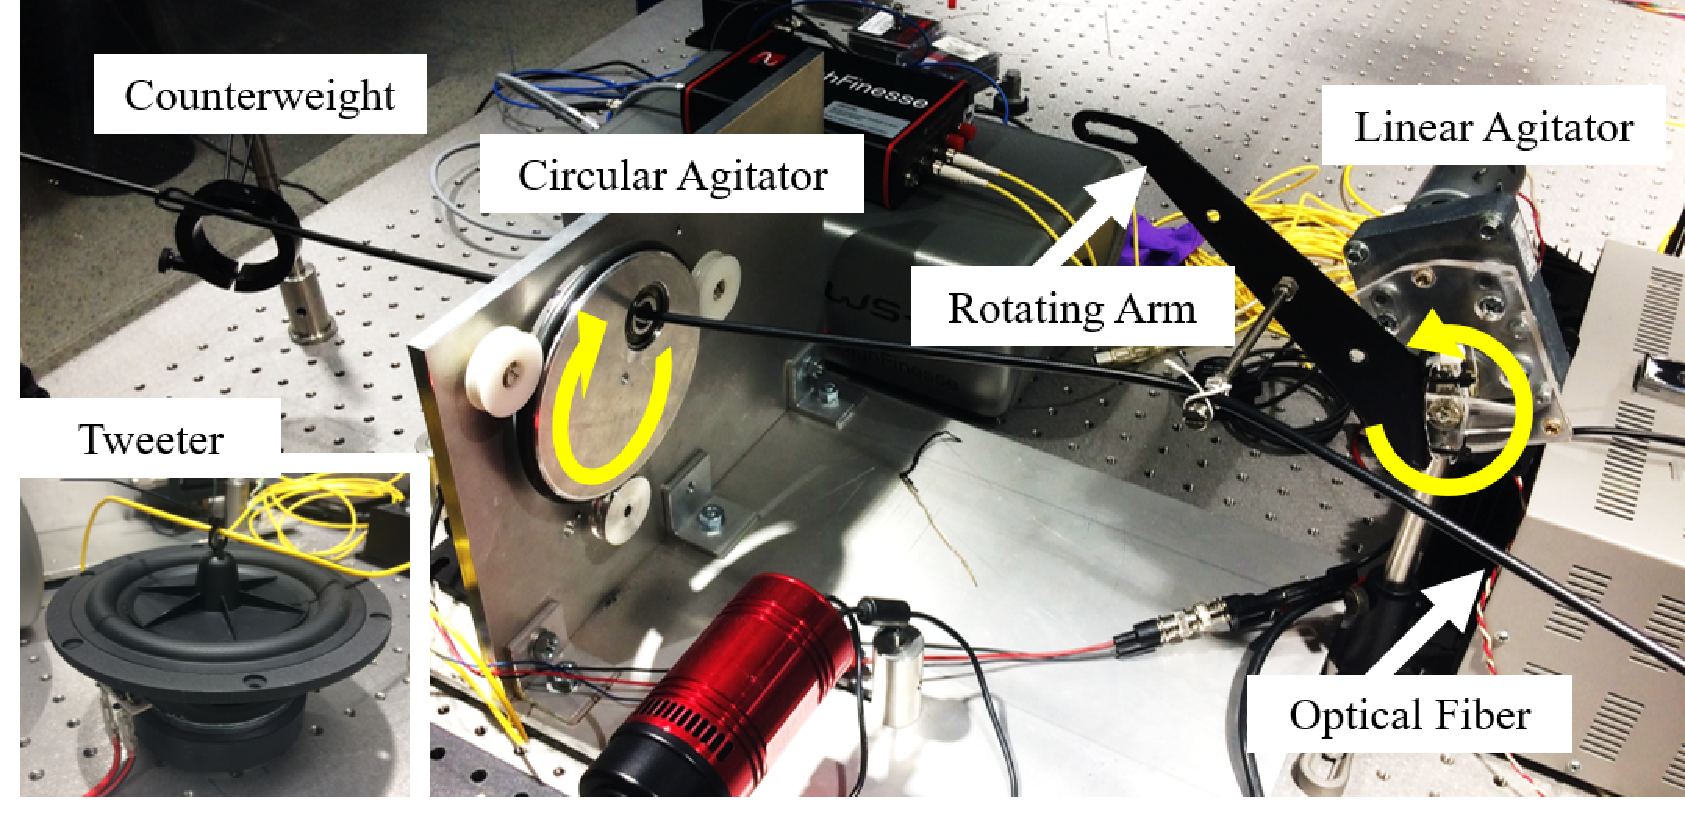
\includegraphics[width=0.97\columnwidth]{figures-2/agitators_labelled.pdf}
	\caption[Photograph of modal noise testing equipment]{Laboratory images of the linear and circular agitator used in these modal noise tests attached to the \SI{100x300}{\micro\meter} rectangular fiber. The linear agitator rotates a variable-amplitude arm parallel to the fiber while the circular agitator rotates perpendicular to the fiber. A small counterweight keeps a minimal amount of tension in the fiber and prevents it from over-bending or bunching up. The inset in the bottom left contains a PASCO Scientific economy wave driver (``tweeter'') attached to an optical fiber. The tweeter is used to test high-frequency, low-amplitude agitation.}
\label{fig:agitators}
\end{figure}

Two different methods of large-amplitude mechanical agitation are tested (Figure \ref{fig:agitators}): the first produces a linear-type motion in which the fiber is moved up and down, the other is a circular type motion in which the fiber is rotated perpendicular to the direction of propagation. The linear agitator has variable amplitude allowing for 80--\SI{320}{\milli\meter} peak-to-peak amplitude agitation at \SI{80}{\milli\meter} intervals and variable frequency in the range of 0.03--\SI{1.0}{\hertz}. For the circular agitator, the fiber is rotated in a circular path with a set diameter (peak-to-peak amplitude) of \SI{80}{\milli\meter} and a variable frequency from 0.1 to \SI{1.5}{\hertz}. Routing a fiber through both agitators produces what we call ``coupled agitation.''  Frequencies are independently set by adjusting the appropriate DC-motor drive voltage and the amplitude of the linear agitator is set by the position of the lifting arm. A small counterweight is present to keep a minimal amount of tension in the fiber between the agitators and prevent it from folding on itself.

To test high-frequency, low-amplitude agitation, we use a PASCO Scientific ``Economy Wave Driver'' shown in the inset of Figure \ref{fig:agitators}. This device, attached to a sine wave function generator, produces approximately \SI{5}{\milli\meter} amplitude for 10-\SI{30}{\hertz} oscillations. It can be driven at higher frequencies, but the amplitude would not be large enough to produce significant fiber motion. We call this device a ``tweeter'' in homage to \citet{plavchan_precision_2013}.

All image data is collected with the Fiber Characterization Station (FCS, Figure \ref{fig:fcs}), a multipurpose device that is able to simultaneously image the input face, near field, and far field of the fiber under test. For these tests, we feed the FCS with either a \SI{652}{\nano\meter} Toptica diode laser (less than \SI{1}{\mega\hertz} linewidth) through a single-mode fiber or a broadband Thorlabs mounted LED centered at approximately \SI{455}{\nano\meter} through a \SI{100}{\micro\meter} circular fiber. Regardless of light source, the FCS focuses light into the fiber as a \SI{10}{\micro\meter} Gaussian spot. Specifications for the FCS cameras are listed in Table \ref{table:cameras}. According to these specifications, our near-field camera has a spatial resolution of \SI{0.3}{\micro\meter}. However, by subtracting ambient calibration images, strictly thresholding to remove background counts, and comparing the unweighted and weighted centroids of each fiber image (thus removing camera drift), we have yielded fiber-centroiding precision to about \SI{0.01}{\micro\meter}.

\begin{figure}
\centering
	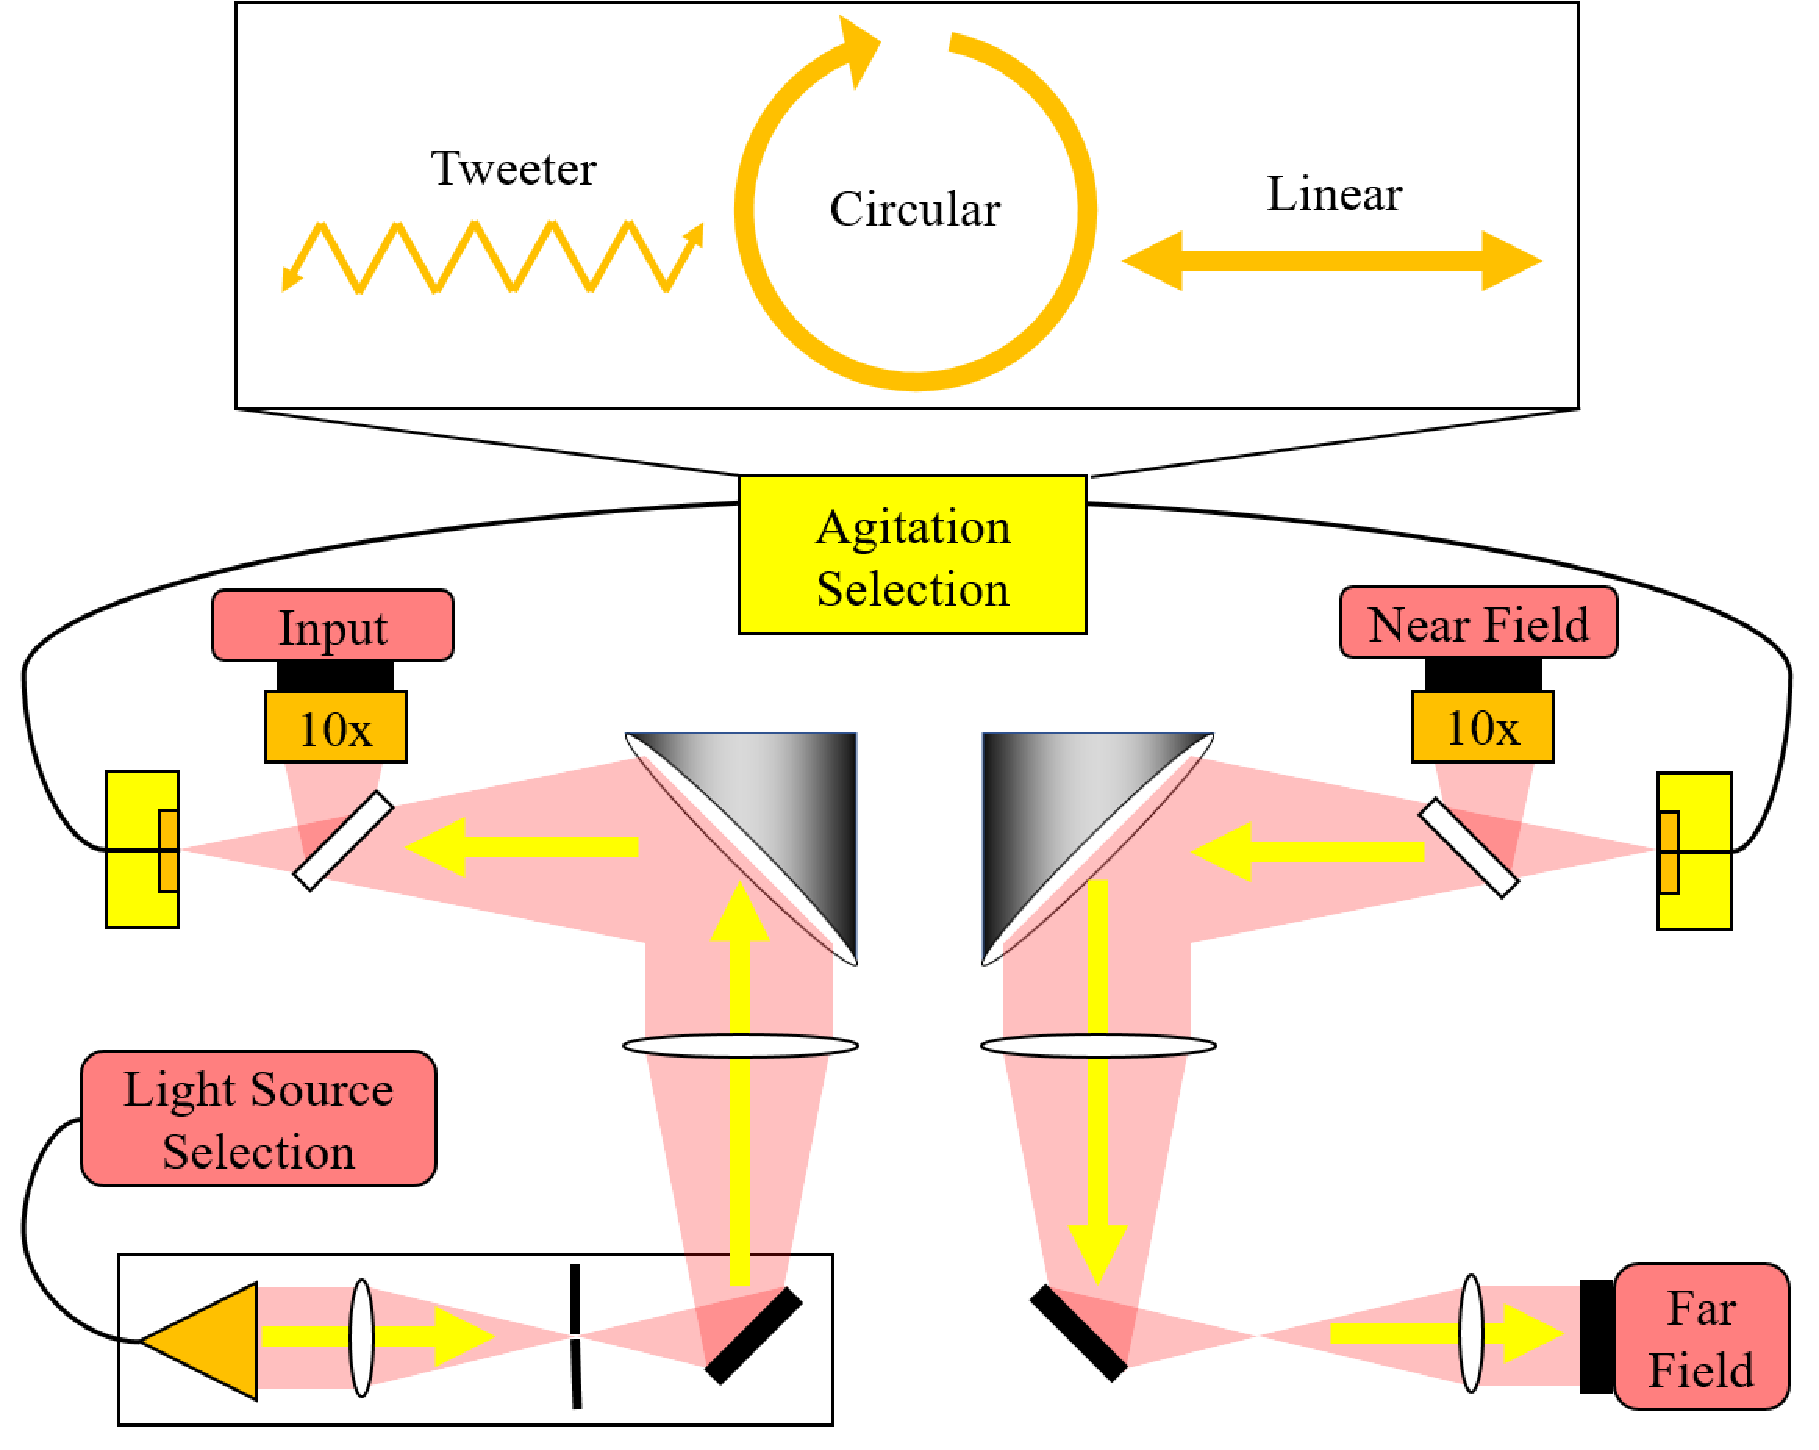
\includegraphics[width=.9\columnwidth]{figures-2/fcs_schematic.pdf}
	\caption[Schematic of the Fiber Characterization Station]{Schematic of the Fiber Characterization Station. Our choice of light source is fed into the station in the bottom left. This light is spatially filtered at focus, collimated (with optional iris for NA selection), and finally injected into the test fiber as a \SI{10}{\micro\meter} spot. The injection face of the test fiber is imaged at $10\times$ magnification by the input camera to allow for precision alignment. Light propagates through the test fiber and our choice of agitator mixes the modes. A cartoon of the three types of agitation (see Figure \ref{fig:agitators}) is presented above the schematic. Light then exits the test fiber and is split between the $10\times$ magnified near-field camera and the far-field camera.}
\label{fig:fcs}
\end{figure}

\begin{table}
\centering
\caption{Fiber Characterization Station imaging specifications}
	\begin{tabular}{llcc}
	\hline
	Name & Camera & Pixel Size & Magnification \\
	\hline \hline
	Input & Atik 450 & \SI{3.45}{\micro\meter} & 10 \\
	\hline
	Near Field & Atik 450 & \SI{3.45}{\micro\meter} & 10 \\
	\hline
	Far Field & Atik 383L+ & \SI{5.4}{\micro\meter} & N/A \\
	\hline	
	\end{tabular}
\label{table:cameras}
\end{table}

Image exposure times are set according to the frequency of agitation such that each exposure lasts exactly one period of rotation. For example, if an agitator is set to rotate at \SI{0.5}{\hertz}, each image will be exposed for \SI{2.0}{\second}. We also scale the intensity of our light source to the set exposure time to minimize the relative effect of read-noise on short exposure images. \citet{baudrand_modal_2001} and \citet{lemke_modal_2011}, as outlined in Section \ref{modal-noise:mn:mitigation}, find that more rotations within the same exposure time improve modal noise. We rather want to see if frequency improves modal noise \textit{per rotation}. Therefore, we control for ``number of rotations'' by confirming exactly one rotation is being recorded.

Each data set is comprised of 10 exposures for each of the following cases:
\begin{enumerate}
\item The fiber being actively agitated.
\item The fiber routed through the agitator but without agitation (``unagitated'').
\item The unagitated fiber illuminated with a broadband LED.
\end{enumerate}
Multiple images are taken (1) to reduce statistical errors in our S/N calculations potentially caused by camera noise or small inconsistencies with our agitators and (2) to observe the effects of agitation at longer exposure times by coadding multiple single-rotation images together. The LED source acts as a control for our S/N and centroiding noise floor, since it is relatively incoherent and thus modal noise is suppressed when using wavelength-integrating cameras, and the unagitated fiber acts as a worst-case scenario.

\begin{figure}
\centering
	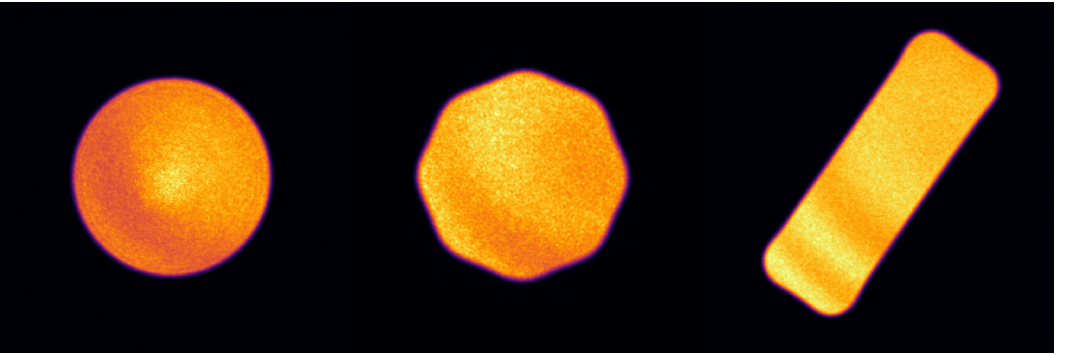
\includegraphics[width=\columnwidth]{figures-2/fiber_improved.pdf}
	\caption[Fiber faces with mitigated modal noise]{10-rotation, coupled agitation images using the same three fibers shown in Figure \ref{fig:fiber_example}.  The diffraction pattern is clearly seen, but otherwise, the presence of speckles in these images is significantly diminished. Brightness is directly scaled with photon count in these images.}
\label{fig:fiber_improved}
\end{figure}

We quantify modal noise using the S/N of light within the fiber face of the near-field image calculated as
\begin{equation}
\mathrm{S/N} = \frac{\mathrm{median}(I_\mathrm{filt})}{\mathrm{stdev}(I_0 - I_\mathrm{filt})}
\label{eq:snr}
\end{equation}
where $I_0$, the original raw image, is heavily median filtered to produce $I_\mathrm{filt}$. The typical S/N (where the ``signal'' is assumed to be a top-hat function across the fiber face) could not be used due to slight intensity-varying diffraction effects across the near-field image (see Figure \ref{fig:fiber_improved}). The contrast from these diffraction effects is approximately 0.2 and we presume they are caused by the thin-film beamsplitter used on the FCS and not from the fiber itself. Subtracting $I_\mathrm{filt}$ from $I_0$ therefore produces a noise pattern that reflects the modal noise and not these large-scale diffraction-caused variances.

We use a circular 51 pixel median filter rather than a low-order polynomial or Gaussian fit because these latter functions were too smooth to provide a good fit to the raw fiber images. The size of the filter kernel was chosen such that speckles on unagitated images are sufficiently filtered without removing structure from the edges of the fibers. The numerator in Equation (\ref{eq:snr}) is calculated as the median (rather than the mean, for example) of $I_\mathrm{filt}$ to prevent dust on the fiber face or optics from skewing the S/N down.

We calculate the S/N for each individual image and average them together within each data set to yield a single-rotation S/N. We then coadd images 1--2, 1--3, ..., 1--10 and calculate the S/N for each case. The S/N for images 1--10 is presented as the 10-rotation S/N and each intermediate step as two-rotation S/N, three-rotation S/N, etc.

Far-field images are taken for each data set and analyzed using the maximum intensity rather than the median intensity as the numerator in Equation (\ref{eq:snr}). The far-field speckle pattern is of interest in precision RV spectroscopy, as it is what illuminates the optics and thus affects the line spread function of the instrument. Also, the optical far field and near field are not directly correlated, meaning any result in the near field does not automatically extend to the far field. That being said, we found that all results listed in the following section for the near field are identical to those found when using the far field. Also, mapping the far-field speckle pattern to RV error would require numerical simulations with optical design software and is beyond the scope of this paper. Therefore, we omit the far-field data for conciseness.

\section{Results}
\label{modal-noise:results}

\subsection{Method of Agitation and Fiber Geometry}
\label{modal-noise:results:ag-snr}

We compare the two individual agitation methods and coupled agitation using all of the fibers listed in Table \ref{table:fibers}. The linear agitator is set to an amplitude of \SI{80}{\milli\meter} and the frequency of both agitators to \SI{1.0}{\hertz}. All images are taken with \SI{1.0}{\second} exposures.

\begin{figure}
\centering
	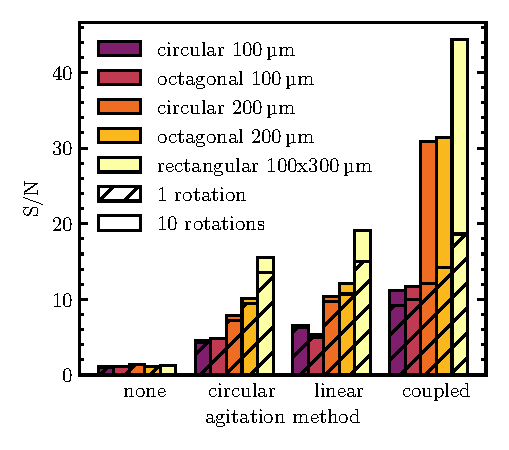
\includegraphics[width=0.7\columnwidth]{figures-2/ag_snr.pdf}
	\caption[Signal-to-noise comparison across fiber geometry and agitation method]{S/N comparison for varying fiber geometries and large-amplitude agitation methods. The S/N is presented for both single-rotation and 10-rotation images.}
\label{fig:ag_snr}
\end{figure}

Results for the single-rotation and 10-rotation cases are shown in Figure \ref{fig:ag_snr}. Across all fiber shapes and sizes and number of rotations, the linear agitator appears to be slightly better than the circular agitator. There is a similar increase in S/N when looking at coupled agitation in single-rotations. However, coupling the agitation over 10-rotations significantly increases the S/N for all fiber configurations.

\begin{figure}
\centering
	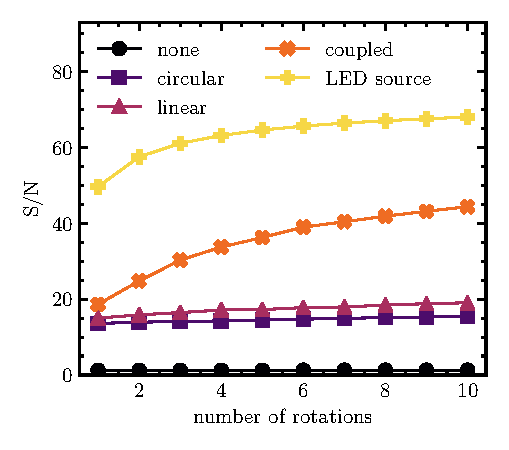
\includegraphics[width=0.68\columnwidth]{figures-2/rect_snr_vs_time.pdf}
	\caption[Signal-to-noise comparison across number of rotations and agitation method]{S/N dependence on number of rotations for the \SI{100x300}{\micro\meter} rectangular fiber using various agitation methods. We find similar relationships for the all of the remaining fiber shapes and sizes.}
\label{fig:rect_snr_vs_time}
\end{figure}

To better understand why coupled agitation is more effective at reducing modal noise at longer exposures, we also analyze the effect of each agitation method over multiple rotations, as shown in Figure \ref{fig:rect_snr_vs_time} for the \SI{100x300}{\micro\meter} rectangular fiber. The S/N shows significant improvement beyond a single rotation when coupling the agitation methods. The rate of this improvement is about the same (if not slightly better) than that when the fiber is lit by an LED, a relatively incoherent source. Circular and linear agitation, on the other hand, effectively plateau after the first rotation. We see identical effects for all of the remaining fiber shapes and sizes.

10-rotation images of the three larger fibers using the coupled agitation method are shown in Figure \ref{fig:fiber_improved}. Compared to those shown in Figure \ref{fig:fiber_example}, the speckle patterns that appear when using coupled agitation are nearly nonexistent.

\subsection{Amplitude and Frequency of Agitation}
\label{modal-noise:results:amp-freq}

We use the \SI{100x300}{\micro\meter} rectangular fiber and the two agitators separately to test the effects of agitation amplitude and frequency of rotation on the S/N. We can only test amplitude on the linear agitator and take an image set for each position on the rotating arm. We test frequency on each of the linear and circular agitators at approximately equally spaced frequencies across their entire frequency range.

\begin{figure}
\centering
	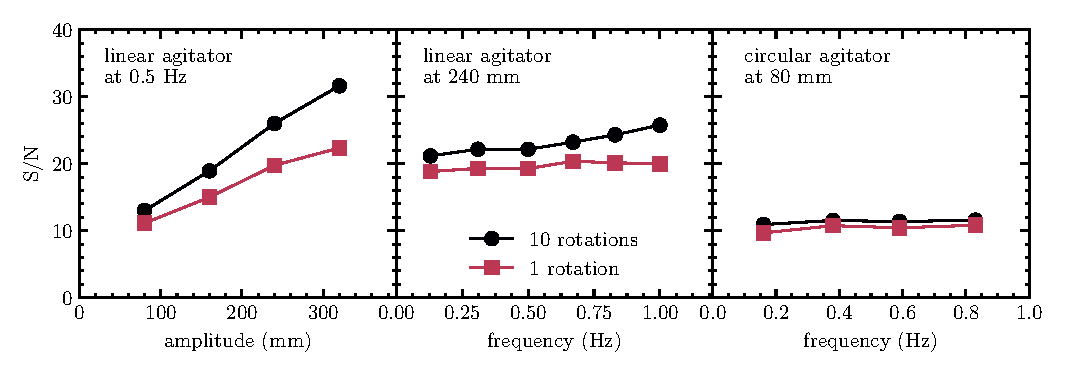
\includegraphics[width=\textwidth]{figures-2/amp_freq_snr.pdf}
	\caption[Signal-to-noise comparison across amplitude and mode of agitation]{S/N comparison for varying amplitudes using the linear agitator (left) and varying frequencies using each of the linear (center) and circular (right) agitators.}
\label{fig:amp_freq_snr}
\end{figure}

Results from these tests are shown in Figure \ref{fig:amp_freq_snr}. There is a strong positive correlation between linear agitation amplitude using both the single-rotation and 10-rotation analyses. There also appears to be a slight increase in S/N for the linear agitator at higher frequencies after ten rotations; however, there is no such increase for the single-rotations or any of the frequencies when using the circular agitator.

\begin{figure}
\centering
	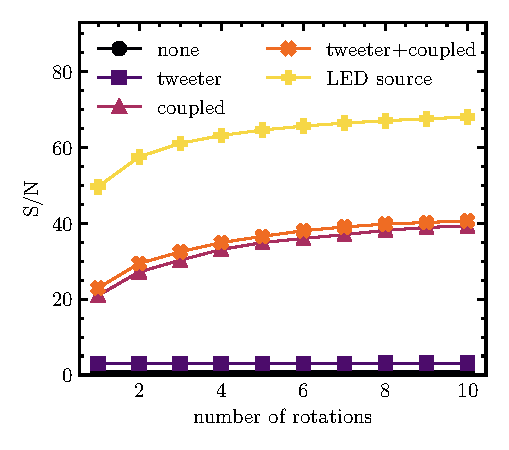
\includegraphics[width=0.7\columnwidth]{figures-2/tweeter_snr.pdf}
	\caption[Signal-to-noise comparison with tweeter]{S/N comparison when adding a tweeter to the coupled agitation method for the \SI{100x300}{\micro\meter} rectangular fiber.}
\label{fig:tweeter_snr}
\end{figure}

We also test the high-frequency, low-amplitude tweeter proposed by \citet{plavchan_precision_2013} in tandem with our coupled agitation to see if it supplies significant additional improvement to S/N. We again exclusively use the \SI{100x300}{\micro\meter} rectangular fiber for this test. We set the linear agitator to \SI{240}{\milli\meter} and \SI{0.5}{\hertz} and the circular agitator to approximately the same frequency. The tweeter is set to \SI{20}{\hertz} which has an intrinsic amplitude of \SI{5}{\milli\meter}. All exposure times are set to \SI{2.0}{\second} to match the rotation periods of the large-amplitude agitators. Therefore, the tweeter oscillates 40 times per exposure.

The results are shown in Figure \ref{fig:tweeter_snr}. The tweeter slightly improves S/N regardless of exposure time when compared to the unagitated fiber and when added to coupled agitation. However, the magnitude of this improvement is minimal and is far outweighed by the improvement due to coupled agitation. Also, this improvement to S/N does not compound over time, but rather adds a constant S/N to the coupled agitation regardless of the combined exposure time.

\subsection{Fiber Coupling}

It is not uncommon for RV spectrographs to have multiple fiber links for carrying calibration and/or science light from the source (lamp or telescope respectively) to the spectrograph and ultimately the detector. This results in having to couple light from one fiber to another and begs the question, is there a preferred fiber to agitate or must we agitate as many as possible? Agitating the first fiber in a multi-fiber system serves to vary the input illumination of subsequent fibers, similar to the methods proposed by \citet{mahadevan_suppression_2014} and \citet{halverson_habitable-zone_2014}. However, agitating subsequent fibers may still be necessary to prevent modal noise from re-emerging.

\begin{table}
\centering
\caption{Fiber assemblies tested for the fiber coupling experiment}
	\begin{tabular}{ccc}
	\hline
	Test & First Fiber & Second Fiber \\
	\hline \hline
	1 & Circular \SI{200}{\micro\meter} & Circular \SI{200}{\micro\meter} \\
	\hline
	2 & Circular \SI{100}{\micro\meter} & Circular \SI{200}{\micro\meter} \\
	\hline
	3 & Octagonal \SI{200}{\micro\meter} & Circular \SI{200}{\micro\meter} \\
	\hline
	\end{tabular}
\label{table:fiber_coupling}
\end{table}

To study the effects of such an architecture, we agitate individual fibers in a multi-fiber assembly where each fiber could have different core sizes and shapes. We test three distinct cases outlined in Table \ref{table:fiber_coupling} and compare them against agitating a single \SI{200}{\micro\meter} circular fiber. For this test, fibers are coupled using one-to-one reimaging optics and fibers are agitated using the linear agitator at \SI{80}{\milli\meter} and \SI{1.0}{\hertz}. When both fibers are agitated simultaneously, they are attached at the same place on the linear agitator, meaning the phase of agitation between the two fibers is constant unlike the previous ``coupled'' agitation tests.

\begin{figure}
\centering
	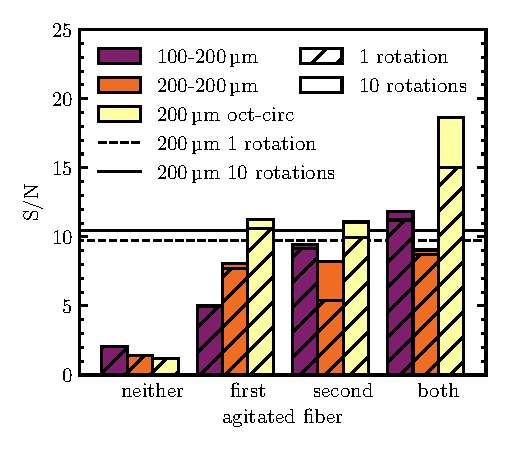
\includegraphics[width=0.7\columnwidth]{figures-2/coupled_fibers.pdf}
	\caption[Signal-to-noise comparison across fiber shapes]{S/N for various arrangements of coupled fibers with varying core diameter and cross-sectional shape. All fibers can be assumed circular unless otherwise stated. The S/N for a single \SI{200}{\micro\meter} circular fiber is also presented for both the singe-rotation (dashed) and 10-rotation (solid) images.}
\label{fig:coupled_fibers}
\end{figure}

The results from these tests are shown in Figure \ref{fig:coupled_fibers}. For the most part, the S/N for each test hovers around 10, the same level at which the S/N would be for an uncoupled \SI{200}{\micro\meter} fiber. However, there are three trends to notice:
\begin{enumerate}
\item When coupling the \SI{200}{\micro\meter} circular fiber to another \SI{200}{\micro\meter} circular fiber, location of agitation does not appear to matter, even if agitating in multiple places.
\item Agitating only the \SI{100}{\micro\meter} circular fiber alone is worse than agitating the \SI{200}{\micro\meter} alone. However, the S/N improves when agitating both of them together.
\item Agitating the \SI{200}{\micro\meter} octagonal fiber or \SI{200}{\micro\meter} circular fiber individually shows no difference in S/N, but agitating both of them significantly improves S/N.
\end{enumerate}
We note that the S/N for single-rotation images when agitating the second fiber in the 200-\SI{200}{\micro\meter} test seems to be abnormally low, but this is alleviated after 10 rotations.

\subsection{Discussion}
\label{modal-noise:results:discussion}

Our results can be summarized as follows: the highest S/N is attained when a fiber has been put through as many physical configurations as possible over the length of an exposure. This is best accomplished using a coupled agitation setup comprised of, in our case, linear and circular motion with the highest amplitude possible on each. Due to the changing phase between the two agitators, the resulting total agitation is effectively chaotic. One could conceive a single-element, random agitator as another possible implementation. Note that the motion needs to be continuous to avoid build-up of a static speckle pattern within the exposure.

This conclusion follows from some of the assumptions addressed in previous studies and introduced in Section \ref{modal-noise:mn:mitigation}. \citet{grupp_nature_2003} actually recommends a chaotic high-amplitude agitator in his statistical study of modal noise. More recently, \citet{lemke_modal_2011}, \citet{mccoy_optical_2012}, \citet{mahadevan_suppression_2014}, and \citet{roy_scrambling_2014} find that hand-agitation is consistently better than any form of mechanical agitation. Human motions are inherently less deterministic than mechanical devices, thus resulting in a more chaotic motion. Our combined linear/circular agitator with slightly different oscillation frequencies mimics this behavior since it chaotically reaches many fiber configurations.

Our results also strongly indicate that larger amplitude is much more crucial to mitigating modal noise than increased frequency, as clearly shown in Figure \ref{fig:amp_freq_snr}. We continue to assert that any periodic rotation used as fiber agitation should complete its cycle within a single detector exposure as originally stated by \citet{baudrand_modal_2001}. However, for single-element agitation, increasing the frequency does not show much of a discernible effect per rotation. We do note that the linear agitator does show a slight positive trend with frequency, but we believe this is caused by small random motions in the fiber further from the agitator that are indirectly intensified by the rapid motions of agitation.

Our tweeter tests also help show the importance of amplitude. Even though the high-frequency device is able to place the fiber into many positions over a single exposure, the difference in these configurations is relatively small. Therefore, the speckle pattern is only ``fuzzed'' rather than averaged over the entire fiber face. Adding a tweeter to a large-amplitude agitator does show some small improvements (since extra ``fuzzing'' would naturally increase S/N), but these improvements are significantly overshadowed by simply having large-amplitude chaotic motion.

We are also able to confirm previous results that show better mitigation of modal noise for fibers with larger cross-sectional areas and less azimuthal symmetry. As seen in Figure \ref{fig:ag_snr}, across all agitation methods, the \SI{200}{\micro\meter} fibers fare better than the \SI{100}{\micro\meter} fibers and the rectangular fiber was consistently far better than the others. Our derived expression for the number of modes (Equation (\ref{eq:mode_area})) accurately describes the ratio between each measured S/N shown in Figure \ref{fig:ag_snr}. For example, Equation (\ref{eq:mode_area}) predicts that doubling the diameter of a fiber should double the S/N, which is precisely reflected in Figure \ref{fig:ag_snr}. We find that the rectangular fiber has approximately $\sqrt{2}$ times the S/N of the circular and octagonal fibers across all agitation methods since $C_\mathrm{rect} \approx 2C_\mathrm{circ}$. Although there is no exact trend, the octagonal fibers tend to have a higher S/N than the circular fibers leading us to believe $C_\mathrm{oct}$ is slightly larger than $C_\mathrm{circ}$.

It follows that the location of agitation in a fiber architecture should be on the fiber that propagates the most modes. We verify this as shown in Figure \ref{fig:coupled_fibers}. When coupling two fibers together that propagate the same number of modes, in our case a \SI{200}{\micro\meter} circular fiber with itself and with a \SI{200}{\micro\meter} octagonal fiber, there is no discernible difference in S/N when agitating one over the other. S/N is significantly worsened, however, when a smaller \SI{100}{\micro\meter} circular fiber is agitated instead. Agitating both fibers appears to combine the improvements to S/N caused by agitating each fiber individually, but only when the two fibers have different size or geometry. When the two fibers are identical, S/N is unaffected.

Moreover, we can infer that the location of agitation along a single fiber does not affect S/N. Coupling two \SI{200}{\micro\meter} fibers with a 1:1 ratio is effectively adding their lengths together and creating a single fiber. As shown by Figure \ref{fig:coupled_fibers}, the location of agitation is irrelevant for such a situation, especially for 10-rotation exposures. Therefore, the agitator could be placed anywhere along the length of the fiber (preferably far away from the spectrograph) and it will produce the same magnitude effect on modal noise. This conclusion relies on only one test, however, so it will require further study to absolutely confirm.

Coupled fiber test cases with light loss due to improperly matched \'etendue, such as coupling light from a \SI{200}{\micro\meter} fiber into a \SI{100}{\micro\meter} fiber, were not covered for this paper and will require further study. However, we suspect that the best modal noise mitigation will consistently occur when agitating the fiber that propagates the most modes, since improvements to modal noise S/N occur across the entire near field and far-field projections and should be unaffected by truncation.

\section{RV Precision}
\label{modal-noise:rv-precision}

\begin{figure}
\centering
	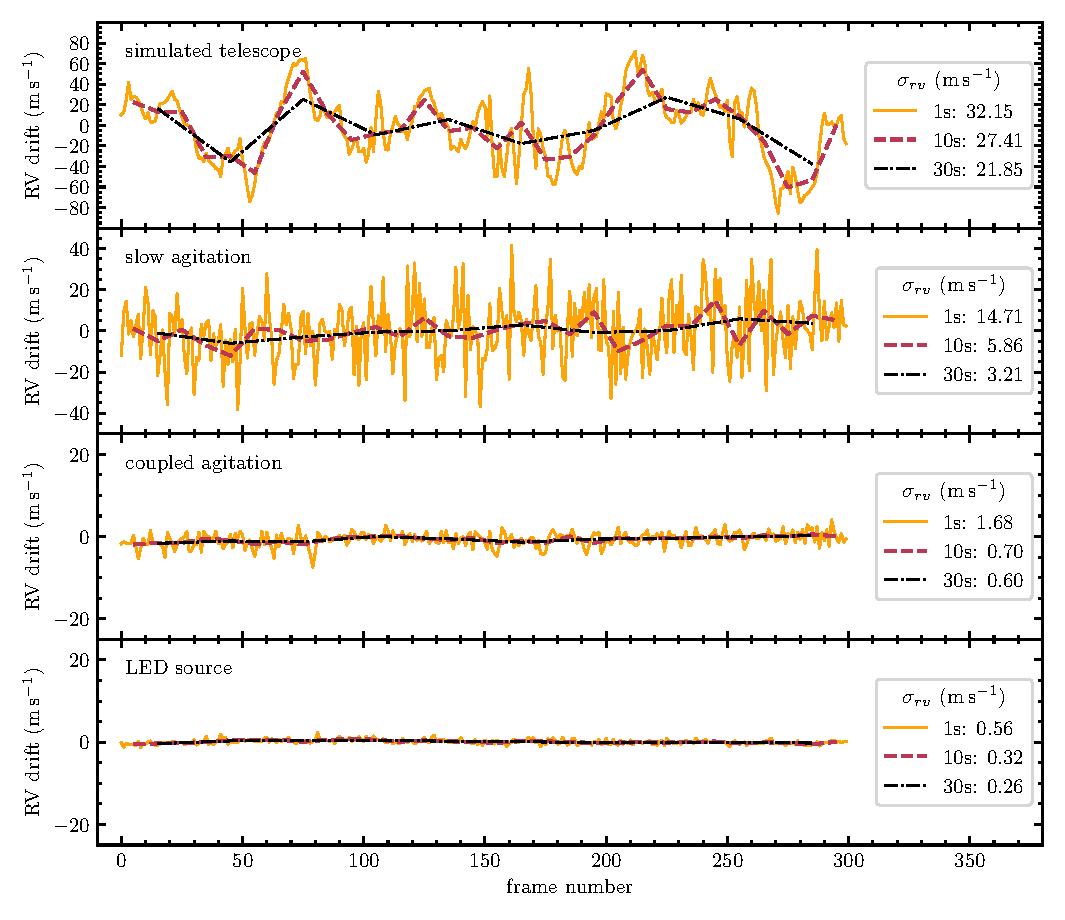
\includegraphics[width=\textwidth]{figures-2/rv_error.pdf}
	\caption[Radial velocity error with and without fiber agitation]{Centroid drift and resultant RV error for a fiber moved by a simulated telescope (first), slowly agitated fiber (second), coupled agitated fiber (third), and LED illumination (fourth). Each line represents a different exposure time each with their own calculated RV error. Note that the scale for the top three plots are different.}
\label{fig:rv_error}
\end{figure}

As discussed in Section \ref{modal-noise:mn}, optical fiber modal noise is an issue of centroid drift as well as diminished S/N. To observe how the centroid actually drifts over time, we test our agitation method on the \SI{100x300}{\micro\meter} rectangular fiber over three hundred \SI{1.0}{\second} exposures.

The resultant RV precision ($\sigma_{RV}$) due to a shifting speckle pattern centroid at the end of a fiber is calculated as
\begin{equation}
\sigma_{RV} \approx \frac{c}{R} \frac{\sigma_d}{D},
\label{eq:rv_error}
\end{equation}
where $c$ is the speed of light in a vacuum, $R$ is the resolution of the spectrograph, $\sigma_d$ is the standard deviation of fiber near-field centroid drift in the dispersion direction, and $D$ is the slit width (or short-end length of a rectangular fiber). Notice that for a $R=150,000$ spectrograph fed by a \SI{33}{\micro\meter} slit attempting to reach \SI{1.0}{\meter\per\second} RV precision per line, the required stability of the centroid along the dispersion direction is \SI{0.0165}{\micro\meter}.

Importantly, $\sigma_{RV}$ is only the RV error \textit{per resolution element} or \textit{per line} from a wavelength calibration source. Averaging over $N$ lines with independent modal structure, we can divide $\sigma_{RV}$ by $\sqrt{N}$ to approximate total RV error. $N$ may not necessarily equal the total number calibration lines, however, since two neighboring wavelengths may propagate with the same number of modes and thus the same modal structure. Recall from Equation (\ref{eq:mode_area}) that the number of supported modes is a function of wavelength. With a high number (thousands) of propagating modes, we do not expect adding or subtracting a single mode will result in a statistically independent modal noise structure. Though, such a study is beyond the scope of this paper.

However, assuming a difference in 10 supported modes makes the structure effectively independent, we assert
\begin{equation}
N \approx \frac{M_s(\lambda_{min}) - M_s(\lambda_{max})}{10},
\label{eq:N}
\end{equation}
where $\lambda_{min}$ and $\lambda_{max}$ are, respectively, the minimum and maximum wavelengths of the relevant calibration region. Note that the calibration source needs to be sufficiently dense (i.e. the number of lines is greater than $N$) to properly use this approximation. Even though Equation (\ref{eq:N}) has not been empirically tested, since it requires a comprehensive study on the systematic correlation of modal noise, we believe it to be a rather conservative estimate for statistical reduction.

We derive Equation (\ref{eq:rv_error}) from the low velocity approximation of the relativistic Dop\-pler effect
\begin{equation}
\frac{\Delta \lambda}{\lambda} = \sqrt{\frac{1 + v/c}{1-v/c}} - 1 \approx \frac{v}{c},
\label{eq:doppler_effect}
\end{equation}
where $\Delta \lambda$ is the measured shift in wavelength at wavelength $\lambda$ on the spectrograph for a star moving at velocity $v$ relative to Earth. The resolution of a spectrograph is
\begin{equation}
R = \frac{\lambda}{\Delta \lambda_R},
\label{eq:resolution}
\end{equation}
where $\Delta \lambda_R$ is the width of the spectrograph resolution element in terms of wavelength bandwidth. Centroid shifts in the near field of the fiber face can thus be equated to a measured wavelength shift at the focal plane of the spectrograph:
\begin{equation}
\frac{\Delta d}{D} = \frac{\Delta \lambda}{\Delta \lambda_R}.
\label{eq:spx_shift}
\end{equation}

Combining Equations (\ref{eq:doppler_effect})--(\ref{eq:spx_shift}) we show that
\begin{equation}
\frac{v}{c} \approx \frac{\Delta \lambda}{\lambda} = \frac{1}{R} \frac{\Delta \lambda}{\Delta \lambda_R} = \frac{1}{R} \frac{\Delta d}{D}.
\end{equation}
If we take the standard deviation of the data from each side of this equation ($v \rightarrow \sigma_{RV}$, $\Delta d \rightarrow \sigma_d$) and move $c$ to the right side, we get Equation (\ref{eq:rv_error}).

The idealized agitation method we use to test RV precision includes the circular agitator oscillating at \SI{1.1}{\hertz} and the linear agitator set at \SI{240}{\milli\meter} and \SI{1.0}{\hertz}. Keeping the two agitators at slightly different frequencies means that phase between them constantly changes and a large range of fiber configurations are reached after about \SI{10}{\second}.

We compare this idealized method to the LED source (low modal noise), a slowly agitated fiber (high modal noise), and a fiber moved as if it were attached to a telescope (very high modal noise). For the slow agitation test, we set only the linear agitator at \SI{80}{\milli\meter} and \SI{0.03}{\hertz} meant to simulate a worst-case simple harmonic agitation method. To simulate the telescope motions, we use the linear agitator with \SI{80}{\milli\meter} amplitude but do not rotate continuously. Rather, we leave the agitator off most of the time except to turn it on briefly (about a quarter or half rotation) every 50 images. This approximates two conditions of the telescope: nearly still while tracking a star and sudden motion while switching targets.

To calculate the RV error, we first find the centroid within the fiber face for each image, relative to the center of the fiber in order to remove the observable ($\sim 2$ pixel) drift of the fiber stage. We then project this centroid drift along the short axis of the rectangle. We also average these centroids over sets of 10 and 30 images to approximate the centroid drift for longer exposure times. For each length of exposure, we calculate the standard deviation of the centroid drift and convert all values to RV using Equation (\ref{eq:rv_error}). The dispersion direction for a rectangular fiber is along the short end, meaning that the slit width $D$ is \SI{100}{\micro\meter}. The resolution of EXPRES is 150,000 for a \SI{33x132}{\micro\meter} rectangular fiber, so we use $R=50,000$ in Equation (\ref{eq:rv_error}) since our test fiber is three times as wide as the EXPRES fiber in the dispersion direction.

The results, shown in Figure \ref{fig:rv_error}, indicate that continuous agitation is essential to control modal noise. The simulated telescope yields RV errors above \SI{20}{\meter\per\second} that do not average out well with longer exposures. Using our idealized method of coupled agitation reduces errors from slow agitation by about 5--8 times and are so far minimized to about \SI{60}{\centi\meter\per\second} when using \SI{30}{\second} exposures. The minimum RV error we could measure in this test, by using the LED source, was \SI{26}{\centi\meter\per\second}. Therefore, our coupled agitation method is less than a factor of 3 from reaching our noise floor.

The calculated \SI{60}{\centi\meter\per\second} error for coupled agitation is the RV error \textit{per line} in the spectrograph. Thus, the total RV error could be reduced to below \SI{10}{\centi\meter\per\second} with only 36 mode-independent calibration lines. EXPRES is using a laser frequency comb with approximately {\SI{14}{\giga\hertz}} line spacing across 450-{\SI{700}{\nano\meter}} fed by a {\SI{33x132}{\micro\meter}} rectangular fiber at $f/3.0$ resulting in almost 17,000 calibration lines. Applying Equation (\ref{eq:N}), EXPRES will have $N=350$, reducing the expected RV error of the instrument to less than {\SI{3.2}{\centi\meter\per\second}}.

\section{Agitation and FRD}
\label{modal-noise:frd}

There is concern in the RV community that mechanical agitation will exacerbate FRD within fiber architectures. FRD is defined as when the focal ratio of the output of an optical fiber is less than that of the injected light. In RV spectroscopy, this means that the focal ratio of the telescope may not be preserved when transmitting light to the spectrograph and losses due to FRD-induced vignetting could occur.

FRD can be worsened through mechanical deformation \citet{ramsey_focal_1988}, classified as macrobending (changes to the radius of curvature of bends in the optical fiber) or microbending (deformations smaller than the diameter of the fiber). These bends can couple light into previously unrealized modes thus causing dispersion in the fiber's far field. \citet{powell_application_1984}, \citet{engelsrath_attenuation_1986}, and \citet{ramsey_focal_1988} find that macrobending on its own has little effect on FRD. The fear is rather that violently macrobending the fiber (such as through agitation) may stress the fiber and cause microbending, a more severe detriment to FRD.

Although it has been shown by \citet{sablowski_comparing_2016} that their agitator (which has similar frequency and amplitude to our own) has little effect on FRD, we thought it wise to similarly test FRD using our agitator. We use the {\SI{100x300}{\micro\meter}} rectangular fiber and coupled agitation at approximately {\SI{0.5}{\hertz}} for this test. Using the FCS, we image the far field at various injected focal ratios ($f/3.0$, $f/4.0$, $f/5.0$) selected with an iris on the input pupil. We then determine the output focal ratio by calculating the Gaussian beam diameter of the far-field image (where the edges are set at 1/${e^2}$ of the maximum amplitude) and compare this value to images taken with the output pupil iris set to known diameters.

\begin{figure}
\centering
	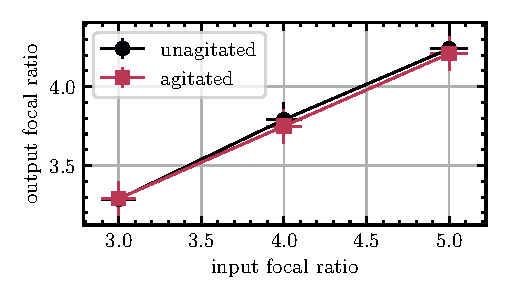
\includegraphics[width=0.7\columnwidth]{figures-2/frd_input_output.pdf}
	\caption[Focal ratio degradation with and without fiber agitation]{Relationship of the input and output focal ratios for the {\SI{100x300}{\micro\meter}} rectangular fiber both with and without agitation.}
\label{fig:frd}
\end{figure}

The results for this test are shown in Figure {\ref{fig:frd}}. Across all three injected focal ratios, the output focal ratio is decreased by less than 0.1 when the fiber is agitated. Thus, there is apparently minimal effect to FRD caused by agitating the fiber with coupled agitation, our most stressful scheme. This does not account for long-term wear-and-tear effects of high-amplitude agitation on FRD, a topic that requires further study, but does show that our coupled agitation method is gentle enough to not cause any immediate devastating issues.

\section{Summary and Application}
\label{modal-noise:conclusions}

We have tested a wide swath of agitation parameter space with the goal of further understanding the mechanisms behind fiber agitation as a method for modal noise mitigation. Our conclusions, as an update to the previous assumptions introduced in Section \ref{modal-noise:mn:mitigation}, are as follows:
\begin{enumerate}
\item Agitating the fiber with the \textbf{most modes}, regardless of its placement in the fiber architecture, yields the best S/N. This typically means the fiber with the largest core size and lowest azimuthal symmetry.
\item \textbf{Large-amplitude} agitation is much more important than high-frequency agitation as long as the agitation method reaches at least one full rotation within an exposure. Adding a ``tweeter'' shows minimal improvement over large-amplitude motion alone.
\item \textbf{Chaotic agitation}, such as the motion created by our ``coupled'' agitator, is much more effective at mitigating modal noise than typical harmonic agitation and continues to improve S/N over multiple rotations. The frequency of this method should place the fiber into as many configurations as possible over a single exposure without over-stressing the fiber.
\item \textbf{Agitating more fibers} in a fiber architecture, especially when the fibers have different geometry (size/shape), will help increase S/N. Using a single agitator with one fiber looped over it several times, however, helps only slightly. Rather, adding a second independent agitator (i.e. chaotic agitation) increases S/N significantly more.
\end{enumerate}

\begin{figure}
\centering
	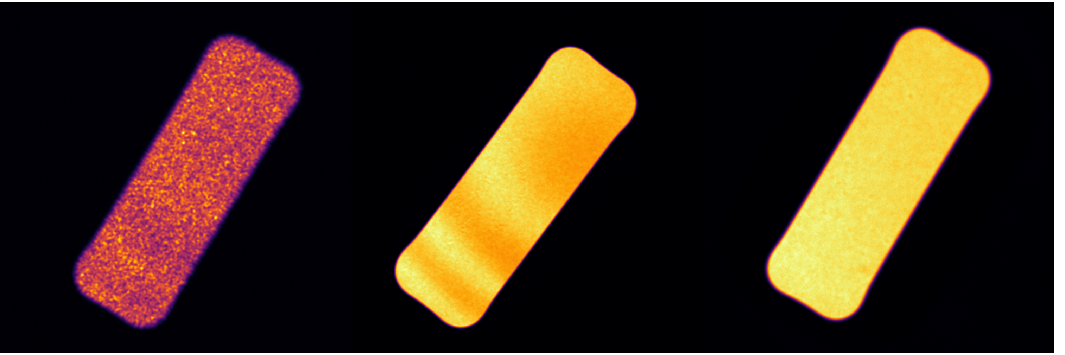
\includegraphics[width=\columnwidth]{figures-2/fiber_rv_error.pdf}
	\caption[Comparison of long-term agitation methods]{Comparison of the long-term agitation methods used in Section \ref{modal-noise:rv-precision}---slow agitation (left), coupled agitation (middle), LED source (right)---as \SI{10}{\second} exposures. Brightness directly scales with photon count in these images.}
\label{fig:fiber_rv_error}
\end{figure}

As shown in Figure \ref{fig:fiber_rv_error}, our two high-amplitude agitators oscillating with varying phase reduce modal noise to levels almost indiscernible from a fiber propagating broadband light after only 10 cycles over an exposure. Since agitation hardly affects throughput efficiency, chaotic fiber agitation can be used with relatively dim light sources, allowing for direct application to the next-generation of precision RV spectrographs.

It is important to note that there has not yet been a long-term study on how shaking an optical fiber may affect attenuation or increase the probability of completely breaking the fiber. We demonstrate that FRD is unaffected in the short-term and, so far, our fibers have not shown detrimental effects due to the aforementioned agitation methods. Our results also show that high-amplitude agitation (i.e. macrobending) in multiple places is more advantageous than quick motions in one location, thus, we believe that microbending---a primary cause of focal ratio degradation---can be more easily avoided. However, any project that wishes to mechanically agitate fibers should take care to avoid over-bending or stretching their fibers and shake them with a minimal amount of aggression.

\begin{figure}
    \centering
    \includegraphics[width=0.75\textwidth]{figures-2/agitator.jpg}
    \caption[The EXPRES fiber agitator]{Picture of the agitator installed with EXPRES at the Lowell Discovery Telescope. The fiber is restrained by rubber bands in this image, but a recent update replaced those with longer-lasting springs. Also, the white arms of the agitator have been replaced by disks with radii equal to the length of the arms. These disks prevent the optical fiber from getting caught on the motor shafts.}
    \label{fig:agitator}
\end{figure}

As part of the EXPRES fiber architecture, we have employed a modal-noise mitigation device influenced by the quasi-chaotic agitation technique detailed in this paper. As shown in Figure \ref{fig:agitator}, the agitator has two arms that each rotate independently using separate voltage-controlled DC motors. We have set these arms to rotate at \SI{0.45}{\hertz} and \SI{0.5}{\hertz} for every exposure, including wavelength calibration, flat-fielding, and stellar observations. These frequencies were chosen to maximally change the phase between the two arms within every exposure without over-stressing the fibers. The agitator has been in use since the beginning of 2018 and there has yet to be any sign of long-term fiber degradation caused by agitation. We also require that all wavelength calibration observations, including from the laser frequency comb and Thorium-Argon lamp, are longer than 10 seconds to ensure sufficient agitation. 

\begin{figure}
    \centering
    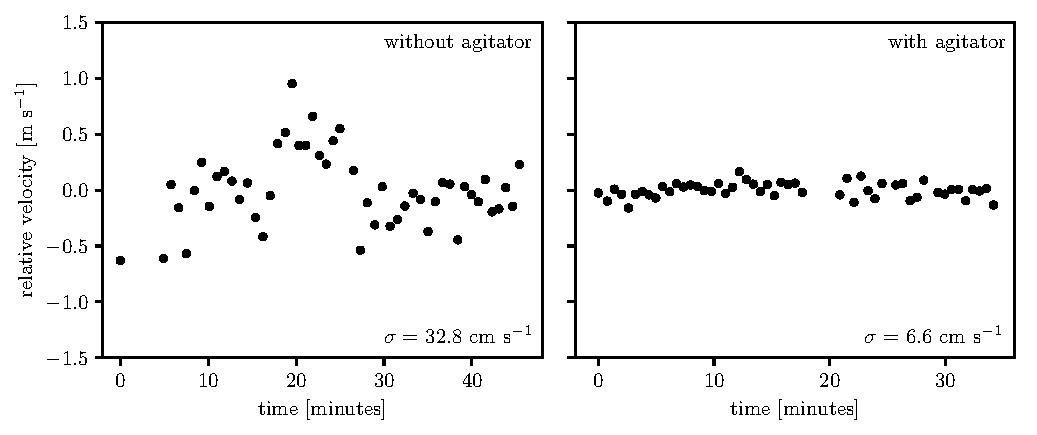
\includegraphics[width=\textwidth]{figures-2/lfc_agitator_comp.pdf}
    \caption[EXPRES stability with and without fiber agitation]{Comparison of instrument stability from cross-correlating LFC exposures without fiber agitation (left) and with fiber agitation (right). Fiber agitation improves the velocity scatter by a factor on the order of 10, reducing this error source to a level below a few cm s$^{-1}$. Image and caption reprinted from \citet{blackman_performance_2020}.}
    \label{fig:lfc-agitator-comp}
\end{figure}

In order to test the effect of this agitation mechanism on the EXPRES wavelength solution and resultant radial velocities, we took a series of observations of the spectrograph's laser frequency comb with the agitator turned both off and on. After extracting each spectrum (see Chapter \ref{chapter:pipeline}), we assigned a displacement velocity for each observation---relative to the first observation of the series---by cross-correlating each spectrum against an analytic template. A linear trend \citep[caused by slow instrumental drifts, see Chapter \ref{pipeline:wavelength-calibration} and][]{blackman_performance_2020} was subtracted for each series and the resultant standard deviation of each series was calculated. As shown in Figure \ref{fig:lfc-agitator-comp}, these are 32.8~\si{\centi\meter\per\second} with the fiber agitator off and 6.6~\si{\centi\meter\per\second} with the fiber agitator on, improving the velocity scatter by about 5 times, comparable to the improvement predicted in Figure \ref{fig:fiber_rv_error} between slow agitation and coupled agitation.

We recommend that other precision RV spectrographs consider the results found in this paper when designing their own fiber agitators. Since it only affects the fibers between light sources and the spectrograph, such improved agitation methods can even be added to previously commissioned spectrographs to increase S/N and reduce potential false positives. We would recommend simply adding a second independent agitator anywhere along the fiber train to help induce more chaoticism. Modal noise is not a problem that should be treated lightly, as its mitigation will help usher in the next-generation of RV spectroscopy and aid in the search for Earth-sized worlds.

\section*{Acknowledgements}

We would like to acknowledge NSF Major Research Instrumentation Award AST 1429365, as well as an NSF Advanced Technologies Instrumentation Award AST 1509436. The author would also like to acknowledge Gabor Furesz for assistance with the Fiber Characterization Station design, Saki Kamon and Kristoffer Acu\~na for their data-taking contributions to this project, and the anonymous referee for their thorough comments. The Fiber Characterization Station was built with support from the Fund for Astrophysical Research, Inc. This material is based upon work supported by the National Science Foundation Graduate Research Fellowship under Grant No. 2017242370.

	\chapter{Aluminum Nitride as a Platform to Support RV Spectroscopy} \label{chapter:astro-comb}

\section{Introduction} \label{astro-comb:intro}

The study of precise and accurate synthetic wavelength calibrators---sometimes endearingly called astro-combs when applied to radial-velocity spectrographs---has been critical to the steady improvement in radial-velocity measurement precision \citep{mccracken_decade_2017}. Commonly, this has been through the application of erbium- or ytterbium-fiber lasers in tandem with feedback-controlled Fabry-P\'erot cavities to increase the mode spacing from $\sim$250~\si{\mega\hertz} to more than 10\si{\giga\hertz} and photonic crystal fibers to broaden the spectral bandwidth. HARPS, EXPRES, and NEID, for example, all use similar calibration combs developed by Menlo Systems based on the work of \citet{probst_laser_2014}. Alternatively, titanium-sapphire lasers can provide $\sim$1~\si{\giga\hertz} intrinsic line spacing, lessening the demand on mode filtering to produce lines detectable by high-resolution spectrographs. HARPS-N \citep{doerr_performance_2012} and HRS \citep{mccracken_wavelength_2017} use such designs.

Ideally, one would be able to produce a $>$10~\si{\giga\hertz} frequency comb directly without the need for complex filtering through feedback-controlled Fabry-P\'erot etalons. This is exactly the promise of electro-optic modulation frequency combs and chip-scale optically nonlinear waveguides, and why these technologies have become popular avenues of development to support radial-velocity spectrographs. So far, the application of electro-optic modulation astro-combs has been limited to near-infrared spectrographs, such as PARVI \citep{yi_demonstration_2016} and GIANO-B \citep{obrzud_broadband_2018}. However, there has also been increasing interest in finding ways to expand these near-infrared combs into the visible regime, especially through the use of silicon nitride waveguides \citep{carlson_ultrafast_2017, obrzud_visible_2019}. These sorts of waveguides are able to leverage optical nonlinearity to both broaden and frequency convert (double/triple) the near-infrared combs.

In this Chapter, I introduce aluminum nitride as an alternative to silicon nitride for astro-comb research development and inclusion in future radial-velocity spectroscopy applications. In Chapter \ref{astro-comb:aln}, I provide some background on aluminum nitride and why it is promising for use in visible radial-velocity spectroscopy. In Chapter \ref{astro-comb:micro-ring}, I describe testing completed with an aluminum nitride microresonator, or micro-ring, on EXPRES to confirm comb viability in blue and ultraviolet wavelength regions. Finally, in Chapter \ref{astro-comb:eom}, I introduce a high repetition-rate electro-optic modulation comb built to test aluminum nitride waveguides for potential application with visible-wavelength spectrographs.

\section{Aluminum Nitride} \label{astro-comb:aln}

The polarizability ($P$) of a material, how much its molecules form electric dipole moments when interacting with light, can be described by a relationship between the material's electric susceptibility ($\chi_0$) and the electric field ($E$). When the material is said to be ``nonlinear,'' this relationship is Taylor expanded and written as
\begin{equation}
    P \approx \epsilon_0 \left( \chi^{(1)} E + \chi^{(2)} E^2 + \chi^{(3)} E^3 + ... \right)
    \label{eq:polarizability}
\end{equation}
where $\epsilon_0$ is the the constant electric permitivity of free space, $\chi^{(1)}$ is the material's linear susceptibility, and higher-order $\chi^{(n)}$ are its nonlinear susceptibilities. 

Nonzero nonlinear susceptibilities of order $n$ enable the interaction of $n+1$ separate photons propagating through the material, through processes collectively called ($n+1$)-wave mixing (See Figure \ref{fig:nonlinearity}). For example, a $\chi^{(2)}$ susceptibility can cause two photons at the same frequency to combine to produce a photon at twice their individual frequencies, a version of sum-frequency generation that is specifically called second harmonic generation. An important caveat, however, is that all of the photons that interact with an (n+1)-wave mixing process must be phase-matched in order for the mixing to even occur.

\begin{figure}
    \centering
    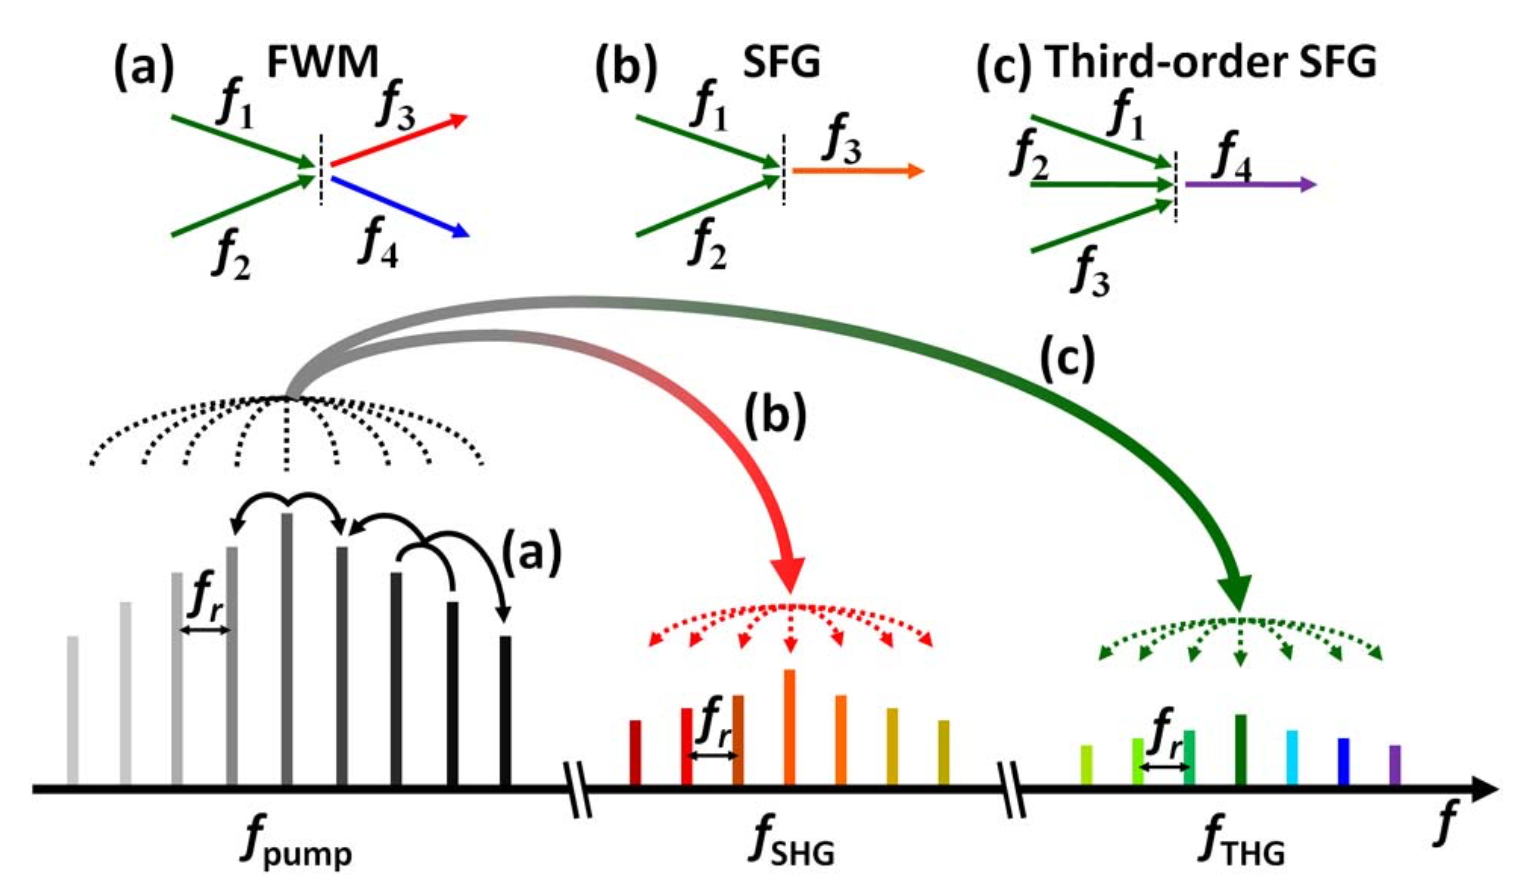
\includegraphics[width=\textwidth]{figures-3/nonlinearity.png}
    \caption[Alumninum nitride frequency conversion diagram]{Diagram of the nonlinear optical processes and frequency conversions that occur within an aluminum nitride waveguide. (a) Side-band generation through cascaded four-wave mixing (FWM) produces a comb centered near the frequency of the pump laser ($f_\mathrm{pump}$). (b) Second-order sum-frequency generation (SFG) produces a comb centered at twice $f_\mathrm{pump}$ (second harmonic generation, SHG). (c) Third-order SFG produces a comb centered at three times $f_\mathrm{pump}$ (third harmonic generation, THG). The repetition rate ($f_r$) within both comb harmonics is the same as in the pump comb. Image reprinted from \cite{jung_green_2014}.}
    \label{fig:nonlinearity}
\end{figure}

Many materials used to develop on-chip waveguides---including silicon [CITATION], silicon nitride [CITATION], aluminum nitride \citep{jung_aluminum_2016}, and lithium niobate [CITATION]---have relatively large $\chi^{(3)}$, meaning that four-wave mixing processes such as third-order sum frequency generation are quite efficient. In addition to straight waveguide applications of third harmonic generation, these materials are also used to produce microresonators (or micro-rings), small rings in which light at only certain discretely-spaced wavelengths resonate. The circumference of the ring dictates the spacing of the resultant frequencies, where from just a single pump laser, numerous comb lines can be produced. When the generation of adjacent comb lines through this process is efficient enough that they begin to cascade, this is known as supercontinuum generation \citep{dudley_supercontinuum_2006}. Supercontinua can produce extremely broadband frequency combs, sometimes even close to octave-spanning, from a single laser source \citep{li_stably_2017, gong_near-octave_2020}.

Alumninum nitride has two strengths compared to these other materials: (1) a strong $\chi^{(2)}$ nonlinearity and (2) a wide band gap \citep{jung_aluminum_2016}. Due to their centrosymmetric structure, silicon and silicon nitride do not display $\chi^{(2)}$ characteristics. Aluminum nitride, on the other hand, can exhibit both three- and four-wave mixing simultaneously. Also, the band gap of aluminum nitride is wider than that of silicon nitride, enabling higher efficiency of blue and ultraviolet light transmission \citep{liu_beyond_2019}. These two properties combined make aluminum nitride an excellent candidate for astro-comb development, which requires continuity and efficiency over the wide bandpass from the ultraviolet through the near-infrared.

The Yale Nanodevices Laboratory has developed a mature nanofabrication process for aluminum nitride that deposits the material with a silicon dioxide cladding onto silicon dioxide or sapphire chips. Using this process, they have fabricated many on-chip aluminum nitride waveguides with varying lengths \citep[300~\si{\micro\meter}--3~\si{\centi\meter};][]{xiong_aluminum_2012}, thicknesses \citep[330--1500~\si{\nano\meter};][]{pernice_second_2012}, and taper geometries \citep{liu_beyond_2019}. These tests demonstrated strong second-order sum frequency generation with differing wavelength-dependent efficiency (phase-matching) depending on the associated geometries. More recently, they have also developed aluminum nitride micro-rings \citep{jung_optical_2013, guo_second-harmonic_2016}, including one that generated a simultaneous green, red, and infrared combs lines that were distinguishable using a $\sim$50,000 resolution spectrograph \citep{jung_green_2014}.

\section{Aluminum Nitride Micro-ring} \label{astro-comb:micro-ring}

The most important aspect of aluminum nitride's potential usability with spectrograph systems such as EXPRES is its ability to convert infrared light efficiently and transparently throughout the entire band-pass of the instrument. As noted in Chapter \ref{intro:wvln_cal}, the Menlo laser frequency comb used with EXPRES has a stated band-pass of 450--750~\si{\nano\meter}, though in practice this has been shown to be closer to 500--720~\si{\nano\meter}. Therefore, demonstration of comb lines that span bluer than 500~\si{\nano\meter} and redder than 720~\si{\nano\meter} would provide evidence for aluminum nitride's ability to simultaneously calibrate the entirety of the EXPRES spectral format.

\begin{figure}
    \centering
    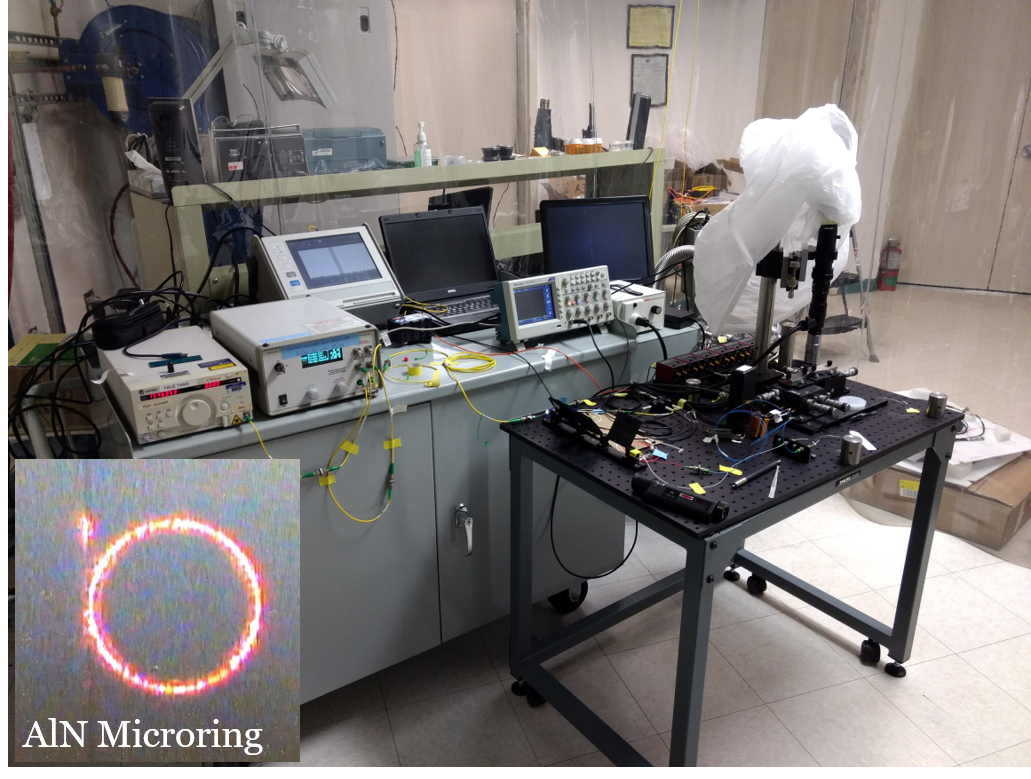
\includegraphics[width=\textwidth]{figures-3/microring-setup.png}
    \caption[Aluminum nitride micro-ring at the Lowell Discovery Telescope]{Image of the aluminum nitride micro-ring setup outside the EXPRES spectrograph room at the Lowell Discovery Telescope. The setup includes a tunable continuous wave near-infrared laser on the very left, immediately next to it is a two stage erbium-doped fiber amplifier, and this is coupled via the components on the optical bench to the aluminum nitride micro-ring. The inset in the bottom left shows a top down view of the micro-ring while it is resonating.}
    \label{fig:microring-setup}
\end{figure}

To do so, we brought an updated version of the aluminum nitride micro-ring introduced in \citet{jung_green_2014} to EXPRES at the Lowell Discovery Telescope during the spectrograph's commissioning in 2018 (Figure \ref{fig:microring-setup}). An amplified tunable continuous-wave near-infrared ($\sim$1550~\si{\nano\meter}) laser is coupled into the device, producing a near-infrared frequency comb that is subsequently doubled ($\sim$780~\si{\nano\meter}) and tripled ($\sim$520~\si{\nano\meter}) throughout the spectral bandwidth of EXPRES. Using a variety of micro-ring geometries---3.4--3.6~\si{\micro\meter} width, 600--800~\si{\nano\meter} gap, 45--60~\si{\micro\meter} radius---we measured the visible frequency comb spectra produced at various resonant pump laser frequencies. In order to highlight certain regions of the spectra without over-saturating other regions on the detector, we used different arrangements of edgepass filters and a wavelength-division multiplexer. Examples of various spectra obtained with EXPRES are shown in Figure \ref{fig:microring-spectra}.

\begin{figure}
    \centering
    \includegraphics[width=\textwidth]{figures-3/microring-spectra.pdf}
    \caption{Spectra of an aluminum nitride micro-ring measured with EXPRES using various configurations of filters and waveguide geometries within three separate wavelength regions of the spectral bandwidth. R, micro-ring radius in \si{\micro\meter}; W, waveguide width in \si{\micro\meter}; G, gap between waveguide and micro-ring in \si{\nano\meter}; $\mathrm{\lambda}$, pump wavelength in \si{\nano\meter}. The blue and orange spectra were taken with a edgepass filter at 650~\si{\nano\meter}. The EXPRES laser frequency comb extends from 5000~\si{\angstrom} to 7200~
    \si{\angstrom}.}
    \label{fig:microring-spectra}
\end{figure}

We found that these configurations of the aluminum nitride waveguide were able to consistently reach from approximately 440~\si{\nano\meter} through the reddest range of EXPRES at 830\si{\nano\meter}. Using the spectral filters, we found relatively high efficiency for both second- and third-harmonic generation of the comb. Unfortunately, this version of the comb does not consistently reach below 440~\si{\nano\meter} except for a few scattered individual lines (see the top plot of Figure \ref{fig:microring-spectra}) likely due to limited broadening of the near-infrared supercontinuum due to the ring. However, the appearance of lines that span redder than 600~\si{\nano\meter} demonstrates aluminum nitride's effectiveness as a frequency doubler and advantage over silicon nitride for astro-comb development.

\section{Electro-optic Modulation Comb} \label{astro-comb:eom}

Rather than rely on a micro-ring to generate a broad enough near-infrared spectrum, we can use near-infrared pulsed laser combs to pump an aluminum nitride straight waveguide, which can be tuned to both broaden and convert the spectrum into the visible regime. \citet{liu_beyond_2019} and \citet{lu_ultraviolet_2020} demonstrated as much with 80~\si{\mega\hertz} femtosecond lasers. However, spectrograph wavelength calibration requires line spacing of more than 10~\si{\giga\hertz}. Therefore, we developed a high-repeition-rate near-infrared electro-optic modulation comb as a pulsed laser source for a straight aluminum nitride waveguide.

\begin{figure}
    \centering
    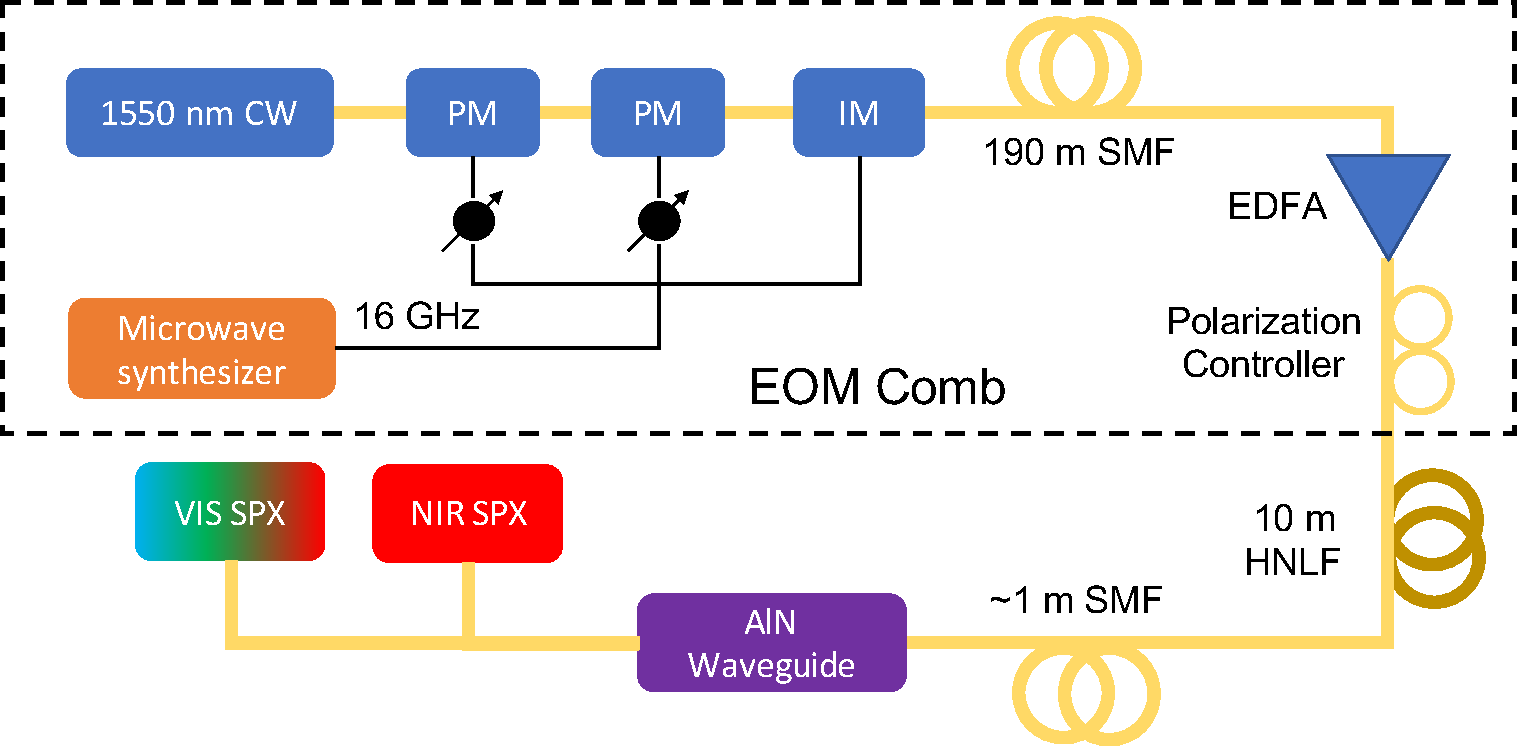
\includegraphics[width=\textwidth]{figures-3/eom-diagram.pdf}
    \caption[Electro-optic modulation comb schematic diagram]{Schematic diagram of the electro-optic modulation comb built for testing with aluminum nitride waveguides. All components within the comb are completely fiber-based, meaning there are no free-space optics until waveguide coupling. EOM, electro-optic modulation; CW, continuous wave laser; PM, polarization modulator; IM, intensity modulator; SMF, single-mode fiber; EDFA, erbium-doped fiber amplifier; HNLD, highly nonlinear fiber; NIR, near-infrared; VIS, visible; SPX, spectrograph.}
    \label{fig:eom-diagram}
\end{figure}

Our electro-optic modulation comb (Figure \ref{fig:eom-diagram}) is designed with a set of off-the-shelf lithium niobate phase (2) and intensity (1) modulators fed by a 1550~\si{\nano\meter} continuous-wave laser. By applying oscillating a voltage across the lithium niobate, we can change the $\chi^{(2)}$ nonlinearity of the material sinusoidally. Depending on the orientation of the lithium niobate crystal structure, either the polarization (which can then be converted to intensity via a polarizer) or phase of propagating light will be modified proportionally to the voltage. The resultant spectrum is a series of side bands surrounding the pump laser frequency separated by the drive frequency of the modulators, which we set to 16~\si{\giga\hertz} using a tunable microwave synthesizer. The relative drive phase of each modulator is matched using independent radio-frequency phase controllers.

The signal coming out of the modulators is chirped, meaning the relative phase of separate frequencies are not aligned, and the intensity of a single pulse is spread out slightly over time. This is corrected by a significant length ($\sim$ 190~\si{\meter}) of single-mode fiber which imparts dispersion compensation opposite that of the chirp. The signal is then amplified using an erbium-doped-fiber amplifier to 3--4~\si{\watt}. In order to broaden the comb before coupling into the waveguide, we send it through 50~\si{\meter} of highly nonlinear silicon fiber. Even though this fiber has nearly zero dispersion, the resultant chirp is again corrected with a short length of single-mode-fiber, minimizing the pulse width at the output of the comb. The optimal length of this final fiber ($\sim$1~\si{\meter}) was determined using a numerical simulation of pulse propagation through the comb. Finally, the optical pulses from this fiber are coupled into an aluminum nitride waveguide using a pair of near-infrared-optimized lenses mounted to a three-axis piezo-controlled alignment stage. Spectra are collected with a combination of near-infrared and visible optical spectrum analyzers.

\begin{figure}
    \centering
    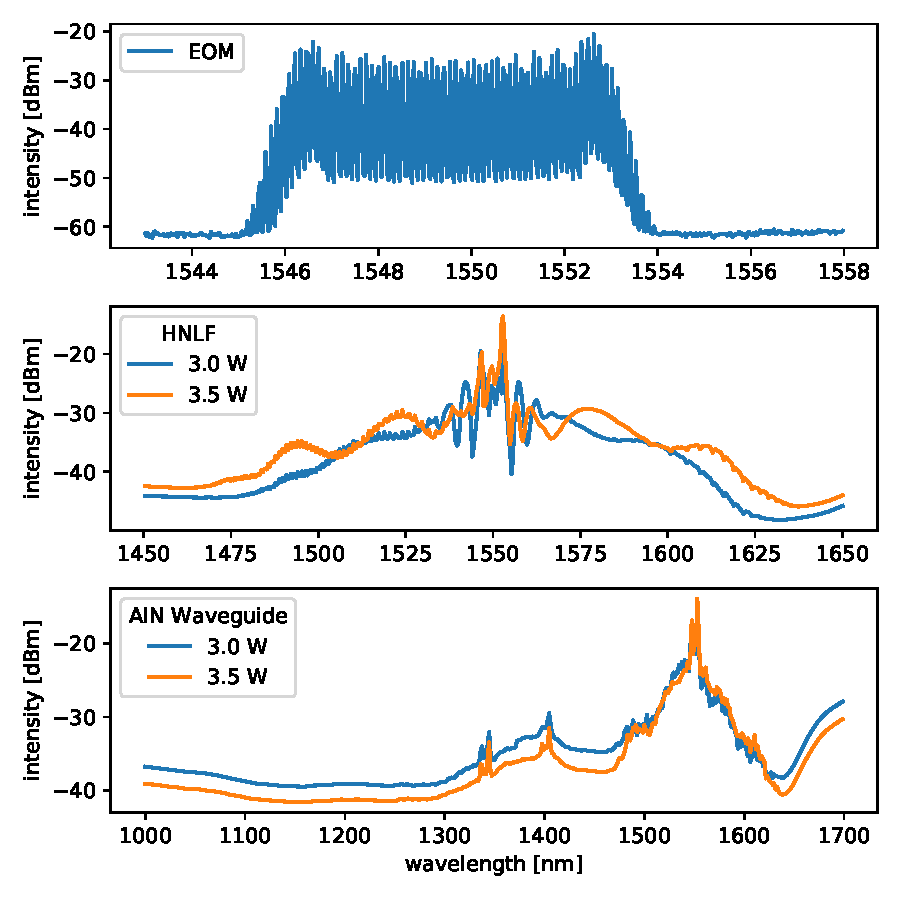
\includegraphics[width=\textwidth]{figures-3/eom-spectra.pdf}
    \caption[Electro-optic modulation comb spectra]{Spectra produce by the electro-optic modulation comb at various points along the optical path. After the electro-optic modulators and single-mode fiber compressor (top), after the highly nonlinear fiber (middle), and after the aluminum nitride waveguide (bottom). Two different amplification power levels are shown for the middle and bottom plots.}
    \label{fig:eom-spectra}
\end{figure}

Output spectra at various stages along the electro-optic modulation comb are shown in Figure \ref{fig:eom-spectra}. Immediately after the electro-optic modulators, the comb bandwidth is approximately 6~\si{\nano\meter}. This is extended to about 100~\si{\nano\meter}, from 1500~\si{\nano\meter} to 1600~\si{\nano\meter}, after amplification and then broadening from the highly nonlinear fiber. The spectrum is not broadened much further by the aluminum nitride waveguide, with some sum-frequency generation occurring around 1400~\si{\nano\meter} and 1340~\si{\nano\meter}. Although not shown here, the 100~\si{\nano\meter} comb around the pump frequency was efficiently converted to a 50~\si{\nano\meter} comb around 780~\si{\nano\meter} and a 33~\si{\nano\meter} comb around 520~\si{\nano\meter}.

\begin{figure}
    \centering
    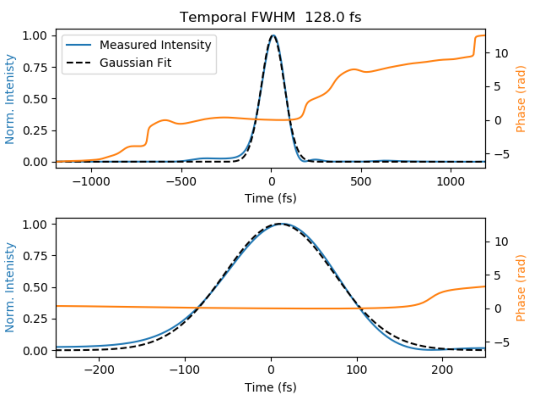
\includegraphics[width=\textwidth]{figures-3/eom-pulse.pdf}
    \caption[Electro-optic modulation comb pulse width]{Pulse width of the electro-optic modulation comb at the point of coupling with the aluminum nitride waveguide. The bottom plot is the same data zoomed in. Gaussian fitting of the line reveals a full-width-half-maximum of about 128~\si{\femto\second}.}
    \label{fig:eom-pulse}
\end{figure}

Measuring the pulse width of the light coupled into the waveguide (Figure \ref{fig:eom-pulse}, we find that it is longer than 120~\si{\femto\second}. Similar electro-optic modulation combs combined with silicon nitride waveguides were able to achieve sub-100~\si{\femto\second} pulses \citep{carlson_ultrafast_2017, obrzud_visible_2019}, meaning our system is likely not tuned enough for maximal pulse compression. We even tested our system on a silicon nitride waveguide similar to the one used by \citet{carlson_ultrafast_2017}, but were not able to achieve an octave-spanning comb. By decreasing the width of the pulse, we could increase the peak power of the signal entering the aluminum nitride waveguide, thereby better exciting its nonlinearity and more likely producing a broader supercontinuum in the near-infrared.

\section{Summary and Discussion}

In summary, we were able to demonstrate the efficacy of aluminum nitride as a candidate for application to radial-velocity spectroscopy wavelength calibration. The aluminum nitride micro-ring tested on EXPRES yielded lines over almost all of the instrument's spectral bandwidth from 440~\si{\nano\meter} to above 820~\si{\nano\meter}, while even occasionally producing lines in the near-ultraviolet. An electro-optic modulation comb, designed to couple into a straight aluminum nitride waveguide, was able to produce a fairly broadband (VALUES) near-infrared frequency comb that could be doubled and tripled to cover the visible regime with significantly less complexity than mode-locked laser frequency comb systems. Unfortunately, broadening of this comb did not reach near-octave bandwidth, likely due to insufficient pulse compression before coupling into the waveguide, meaning a completely viable visible astro-comb design was not achieved.

Although this work was not yet able to generate a extremely broadband visible frequency comb, promising results have been coming from a team at the University of Geneva \citep{obrzud_visible_2019}. Using a completely fiber-based electro-optic system almost identical to the one presented here \citep{obrzud_microphotonic_2019}, they demonstrated complete wavelength coverage from 400--600~\si{\nano\meter} through a silicon nitride waveguide, further demonstrating the material's utility for triple sum-frequency generation. The only other difference between our designs is that they use a chirped fiber Bragg grating over our long single-mode fiber. However, even when we replaced the long single-mode fiber with a dispersion-controller, we were still not able to achieve enough spectral broadening. It therefore appears that the relative lengths of our highly nonlinear fiber and dispersion compensating fibers need to be better tuned to minimize the pulse width before coupling into the waveguide. I would recommend using a longer highly nonlinear fiber to increase this first stage of broadening and then re-optimizing the length of the final single-mode fiber compressor to match the new dispersion profile.

Considering silicon nitride does not have strong second harmonic generation, however, there still remains a space for aluminum nitride within visible radial-velocity spectroscopy. If we could properly tune the electro-optic setup described here, in principle, the combined comb would produce the same 400--600~\si{\nano\meter} blue-green comb as well as a simultaneous 600-900~\si{\nano\meter} red comb. The blue comb may also extend a bit further into the ultraviolet due to the larger band gap. A frequency comb produced by such a device would easily cover the entirety of the EXPRES spectral bandwidth. Unfortunately, due to circumstances created by the pandemic, further astro-comb tuning was not possible within the time-frame of the writing of this thesis.

One possible avenue for future exploration with this technology would be to combine a $\sim$16~\si{\giga\hertz} micro-ring (either aluminum nitride or lithium niobate) with the electro-optic modulation comb. Naturally, this will add more complexity into the system, since the the continuous-wave laser and microwave synthesizer frequency would need to be tuned to match resonance with the micro-ring. However, this may enable greater efficiency in the spectral broadening of the near-infrared comb before converting to visible wavelengths. By continuing research along this track, we may someday soon be able to design an astro-comb completely contained on a single chip-based aluminum nitride waveguide.

Special thanks to Alex Bruch for his significant guidance in learning the ins and outs of nonlinear optics, for contributing his simulation code to this chapter, for joining me in collecting micro-comb data with EXPRES, and for helping me to develop the electro-optic modulation comb. I would also like to thank Zheng Gong for his help in testing the electro-optic modulation comb. I would finally like to thank Scott Diddams and Stephanie Leifer for their guidance through the electro-optic modulation prototyping process.
	\chapter{An Extreme-precision Radial-velocity Pipeline: First Radial Velocities from EXPRES}\label{chapter:pipeline}

\begin{center}
    Adapted from

    \textit{Ryan R. Petersburg, J. M. Joel Ong, Lily L. Zhao, Ryan T. Blackman, John M. Brewer, Lars A. Buchhave, Smanuel H. C. Cabot, Allen B. Davis, Colby A. Jurgenson, Christopher Leet, Tyler M. McCracken, David Sawyer, Mikhail Sharov, René Tronsgaard, Andrew E. Szymkowiak, and Debra A. Fischer}
    
    The Astronomical Journal, Volume 159, Number 5, Page 187, 2020
\end{center}

\section*{Abstract}

The EXtreme-PREcision Spectrograph (EXPRES) is an environmentally stabilized, fiber-fed, $R=137,500$, optical spectrograph. It was recently commissioned at the 4.3 m Lowell Discovery Telescope near Flagstaff, Arizona. The spectrograph was designed with a target radial-velocity (RV) precision of 30\cms. In addition to instrumental innovations, the EXPRES pipeline, presented here, is the first for an on-sky, optical, fiber-fed spectrograph to employ many novel techniques---including an ``extended flat'' fiber used for wavelength-dependent quantum efficiency characterization of the CCD, a flat-relative optimal extraction algorithm, chromatic barycentric corrections, chromatic calibration offsets, and an ultra-precise laser frequency comb for wavelength calibration. We describe the reduction, calibration, and RV analysis pipeline used for EXPRES and present an example of our current sub-meter-per-second RV measurement precision, which reaches a formal, single-measurement error of 0.3\ms for an observation with a per-pixel signal-to-noise ratio of 250. These velocities yield an orbital solution on the known exoplanet host 51 Peg that matches literature values with a residual RMS of 0.895\ms.

\section{Introduction}\label{introduction}

Results from the NASA Kepler mission show that small planets with radii between 1 and 4 $R_{\oplus}$ are found orbiting 20--50\% of main-sequence stars \citep{winn_occurrence_2015}. While such transit surveys, such as Kepler, K2, and TESS, have revealed a wealth of planets, few of these planets have had their masses measured; mass estimates that do exist are typically radial-velocity (RV), dynamical masses. More precise RV measurements are required to determine mass estimates for these planets, particularly small rocky ones, than are possible with pre-existing RV spectrographs. Were they available, these mass measurements would shed light on planetary structure, bulk density, and the mass-radius relation for sub-Neptune-mass planets. 

To meet these needs, a new generation of RV spectrographs is now emerging: the Echelle SPectrograph for Rocky Exoplanets Search and Stable Spectroscopic Observations \citep[ESPRESSO:][]{pepe_espresso_2013} and the EXtreme-PREcision Spectrograph \citep[EXPRES:][]{jurgenson_expres_2016} are now on-sky taking data, while the NN-explore Exoplanet Investigations with Doppler spectroscopy spectrograph \citep{schwab_design_2016} is in the commissioning phase. These new extreme-precision radial-velocity (EPRV) spectrographs are driving toward the sub-10 \cms RV precision needed to detect a true Earth twin around a Sun-like star.

Extremely precise spectrographs, in turn, demand extremely precise data reduction pipelines. The fidelity of the data and error estimates returned by these data reduction pipelines is paramount if groundbreaking discoveries returned from such instruments are to be credible. To this end, a complete science reduction, extraction, and analysis pipeline was newly developed and tailored for EXPRES data. In what follows, we begin with a brief description of the instrument and the calibration strategy. We then describe the analysis performed by our pipeline on EXPRES data, and present the first radial-velocity measurements from the instrument.

\section{Instrument Description}\label{instrument-description}

EXPRES is a fiber-fed, white-pupil EPRV spectrograph with a design resolution of $R = 150,000$ and a wavelength range of $3800-7800~\si{\angstrom}$. In practice, \citet{blackman_performance_2020} show that the median resolution is better characterized as $R \sim 137,500$ with a maximum resolution reaching $R \sim 150,000$ in some regions of the detector. EXPRES is environmentally stabilized in a vacuum enclosure and is situated at Lowell Observatory's 4.3 m Lowell Discovery Telescope (LDT) near Flagstaff, Arizona. The multi-instrument port configuration of the LDT allows for high-cadence, flexible scheduling of stars (up to 280 partial nights per year).

Owing to various changes to the hardware configuration during commissioning, we have divided radial velocities from EXPRES into different calibration epochs, with an independent RV offset fitted for each epoch. Each epoch demarcates changes introduced to the configuration of the echellogram on the CCD, the shape of the point-spread function (PSF), or the stability of our calibration sources. A summary of the changes that delineate the beginning of each epoch can be found in Table \ref{tab:epochs}.

\begin{table}[ht!]
\centering
\caption[EXPRES Instrumental Epochs]{Instrumental Epochs\label{tab:epochs}}
\begin{tabular}{cccl}
\hline
Epoch & Start & End & Changes before Epoch Start \\
\hline
0 & - & 2018 Apr 15 & Commissioning \\
1 & 2018 Apr 15 & 2018 Jun 15 & Increased CCD pre-settle time \\
2 & 2018 Jun 15 & 2018 Nov 8 & Fiber change; \\
 & & & CCD rotation \\
3 & 2018 Nov 8 & 2019 Feb 7 & Original science fiber replaced; \\
 & & &  Calibration unit rebuilt \\
4 & 2019 Feb 7 & 2019 Aug 4 & LFC beat frequency mitigated; \\
 & & &  Fiber agitator repaired \\
5 & 2019 Aug 4 & - & Realignment of FEM; \\
& & &  Replacement of LFC PCF
\\
\hline
\end{tabular}
\end{table}

The inputs to EXPRES are a $33 \times 132 \um$ science fiber as well as a $60 \times 180 \um$ extended fiber. The extended fiber is wider than the science fiber in the cross-dispersion direction, allowing for higher signal-to-noise ratio (S/N) flat-fielding for all pixels illuminated by light from the science fiber, particularly at the cross-dispersion edges. Both fibers are also supplemented by their own square simultaneous fibers, though these are not used in normal operation.

The flat-field light source is provided by a custom solution: a collection of 25 LEDs integrated on a single compact chip. The wavelength range of the LEDs cover the entire bandwidth of EXPRES, and the relative power of each LED is tuned to approximately match the inverse response of the spectrograph. Light from these LEDs, averaging 12.5 W, is coupled into an integrating sphere and subsequently injected into both the extended and science fibers.

Wavelength calibration is carried out with a Menlo Systems laser frequency comb \citep[LFC; similar to those in][]{steinmetz_laser_2008,probst_relative_2016}. Three LFC exposures are taken through the science fiber every 15-30 minutes throughout a night.  Two ThAr exposures are taken each night---once at the beginning and once at the end. The LFC is set to standby between each set of calibrations to reduce wear on nonlinear optical elements, and is only turned on approximately one minute before the next exposure is needed, to suppress turn-on transients.

Barycentric corrections are derived from the EXPRES exposure meter, a $R\approx100$ spectrograph with an EMCCD detector and a bandpass that covers the spectral range of the LFC. During each science observation, the exposure meter takes a continuous series of 1 s exposures. Further technical details can be found in \citet{blackman_measured_2019}.

\hypertarget{analysis-of-expres-data}{%
\section{Analysis of EXPRES Data}\label{analysis-of-expres-data}}

\begin{figure}
    \centering
    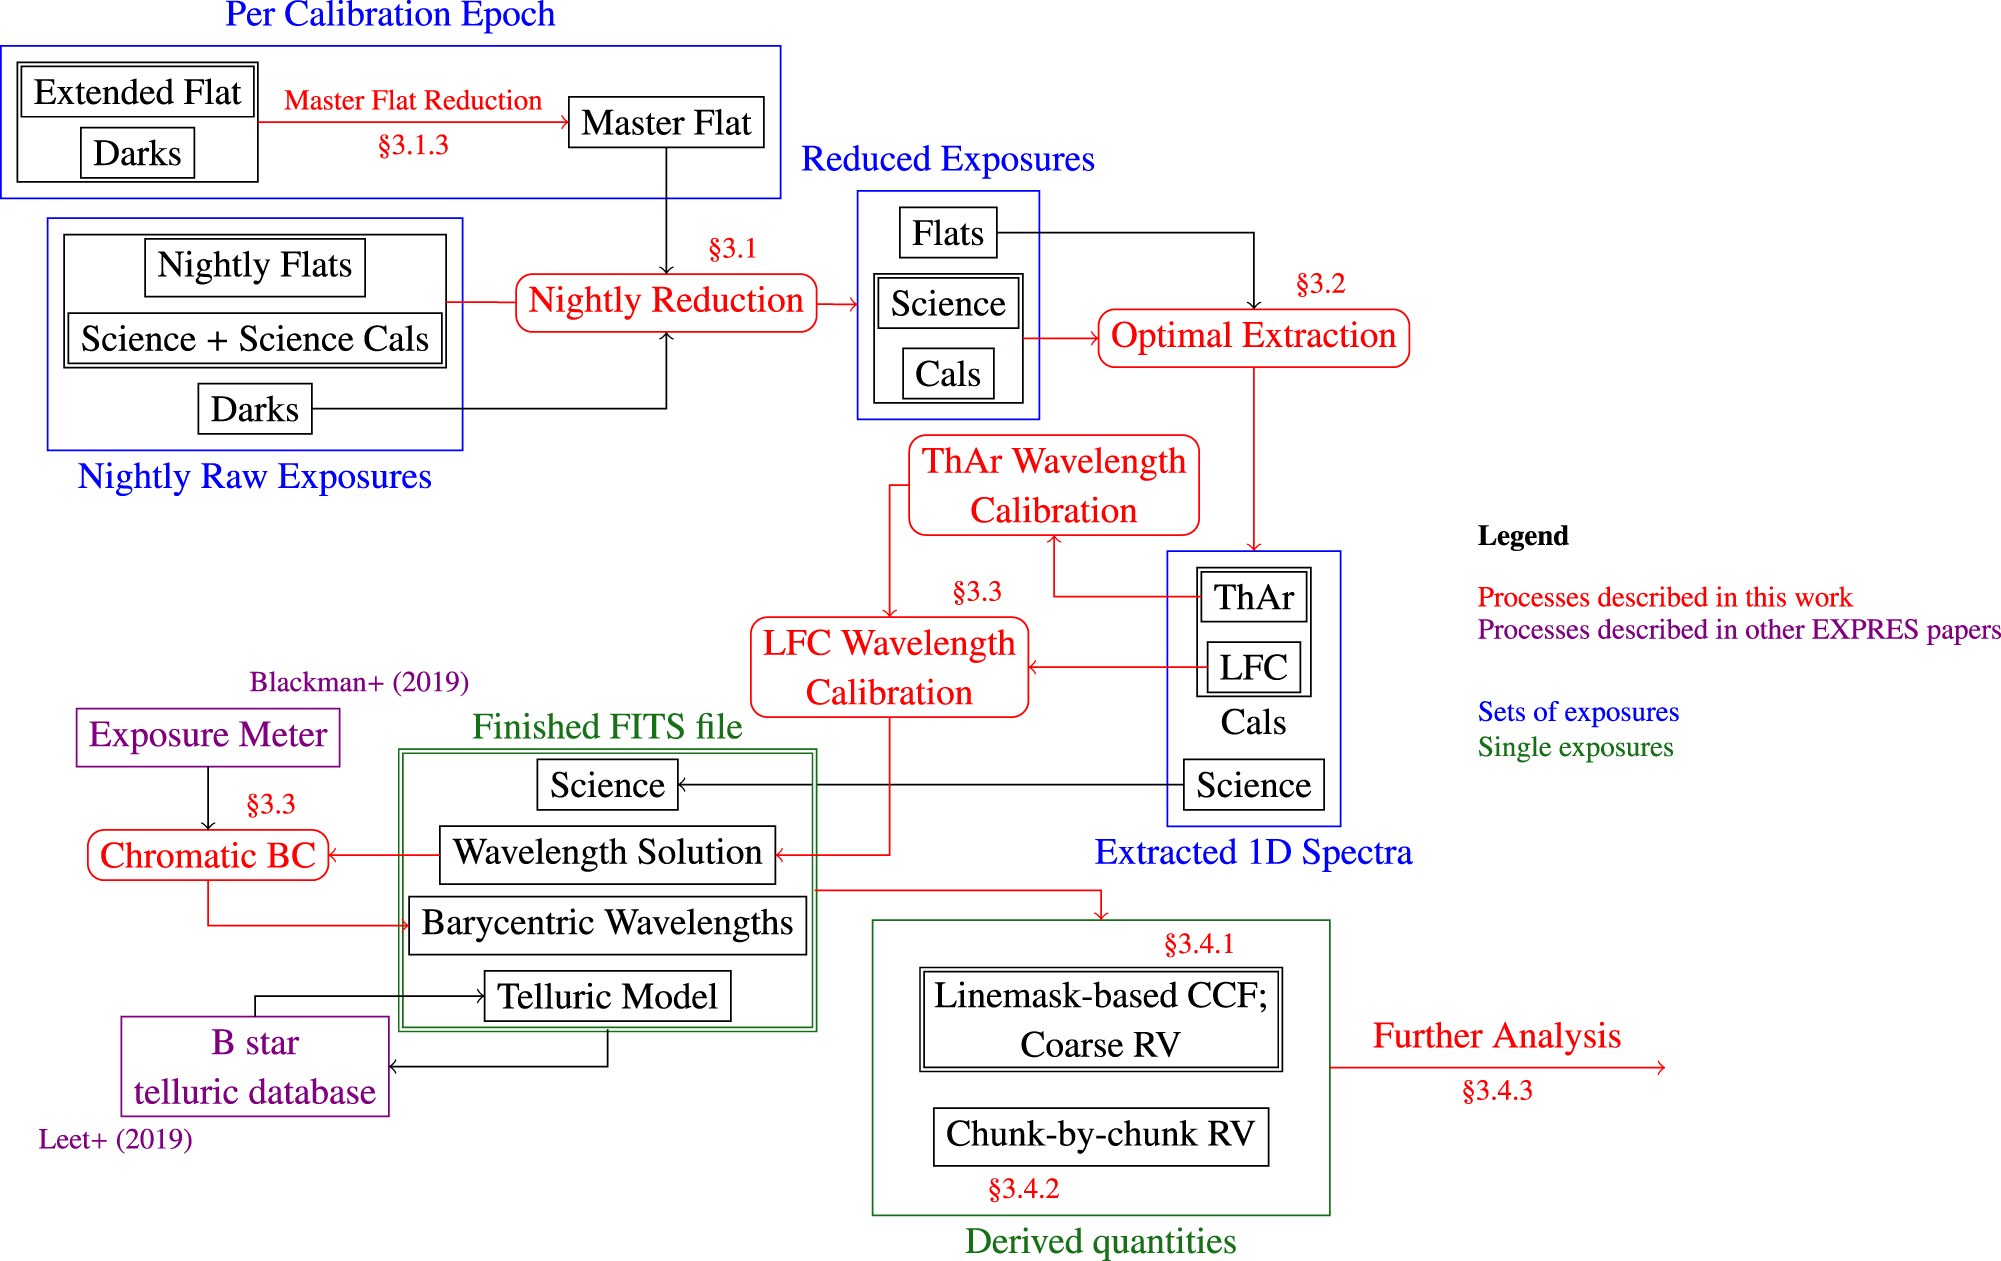
\includegraphics[width=\textwidth]{figures-4/pipeline}
    \caption[Data flow for the EXPRES pipeline]{Data flow for the EXPRES pipeline. Small black boxes represent different kinds of exposures (if in blue boxes) or different data associated with an exposure (if in green boxes). Double-boxes indicate finished data products, ready for use in subsequent science analysis.\label{fig:flowchart}}
\end{figure}

The EXPRES pipeline is written in Python and makes heavy use of the SciPy stack \citep{virtanen_scipy_2020}. We show a schematic representation of it in Figure \ref{fig:flowchart}. In brief, the following steps are taken:

\begin{enumerate}
\item At the start of each calibration epoch, several hundred extended flat images are taken. These are used to construct a master extended flat-field image, which is divided out from all exposures in the corresponding calibration epoch.
\item Each night, 30 dark and 30 science flat images are taken. They are used to reduce and extract the science frames taken the same night.
\item Echellogram orders are traced using the reduced science flats, a scattered light model is removed, and a flat-relative optimal extraction is performed. 
\item Wavelength solutions are interpolated for all science frames using bracketed LFC exposures, seeded by a nightly Thorium Argon source, as a calibration reference.
\item Telluric lines are identified empirically with SELENITE \citep{leet_toward_2019} and labeled for later analysis.
\item For exposures marked for RV analysis, we obtain radial velocities with two methods: cross-correlation against a line mask and a forward model.
\end{enumerate}

We describe each of these steps in the following sections.

\hypertarget{reduction}{%
\subsection{Reduction}\label{reduction}}

The EXPRES detector is an STA1600LN CCD backside-illuminated image sensor with a $10,560 \times 10,560$ array containing $9 \um \times 9 \um$ pixels. The CCD is divided into 16 equal $5280 \times 1320$ pixel sections (two rows of eight), each with their own independent output amplifier and, thus, corresponding gain (see Table \ref{tab:gain}). Further information about the EXPRES CCD can be found in \citet{blackman_performance_2020}.

In the context of the EXPRES pipeline, ``reduction'' refers to the conversion of these 16 independent regions read in analog-to-digital units (ADU) to a full two-dimensional frame in units of photoelectrons. The reduction steps are as follows, dependent on the type of image being reduced (science, dark, science flat, or extended flat):
\begin{enumerate}
    \item Subtract a bias frame constructed from the overscan regions (all).
    \item Multiply each amplifier region by the corresponding gain coefficient (all).
    \item Median combine calibration frames (dark, science flat, extended flat).
    \item Subtract the reduced dark image (science, science flat, extended flat).
    \item Divide by the reduced master extended flat (science, science flat).
    \item Approximate the noise model using photon (Poisson) and read noise (science, science flat).
    \item Trace the echelle orders (science flat).
    \item Approximate the scattered light using a two-dimensional b-spline model (science, science flat).
\end{enumerate}

In the following subsections, we go into detail about each of the above steps. Information about the reduction of exposure meter data can be found in \citet{blackman_measured_2019}.

\subsubsection{Overscan}\label{overscan}

Each of the EXPRES CCD amplifier regions have overscans along both the serial (horizontal) and parallel (vertical) registers. The serial overscan is $5300 \times 180$ pixels along the right side of each amplifier region, and the parallel overscan is $20 \times 1320$ pixels along the center line of the CCD (at the bottom of the upper regions and the top of the lower regions). Because these overscans contain virtual pixels read out by the same electronics as the real amplifier region, the EXPRES reduction pipeline uses them to approximate the bias of the CCD.  The process is as follows:
\begin{enumerate}
    \item Calculate the mean of the serial overscan region along its horizontal axis.
    \item Smooth this mean using a cubic b-spline with knots every $\sim 100$ pixels.
    \item Correct the rows in the parallel overscan region by subtracting the overlapping smoothed serial overscan region.
    \item Calculate the mean of the parallel overscan region along its vertical axis.
    \item Smooth this mean using a cubic b-spline with knots every $\sim 100$ pixels.
    \item Construct a bias for each pixel in the amplifier region by summing the corresponding row from the serial overscan and column from the parallel overscan.
\end{enumerate}
The mean and subsequent spline fit for the overscan regions of a single amplifier region are shown in Figure \ref{fig:overscan}. This process is executed for all exposures, including darks.

\begin{figure}
    \centering
    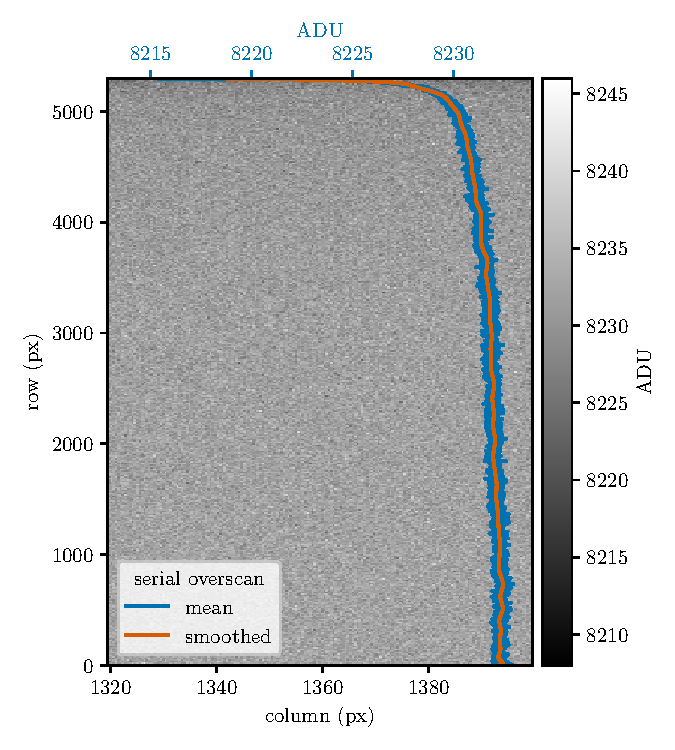
\includegraphics[width=0.65\textwidth]{figures-4/ser_oscan}
    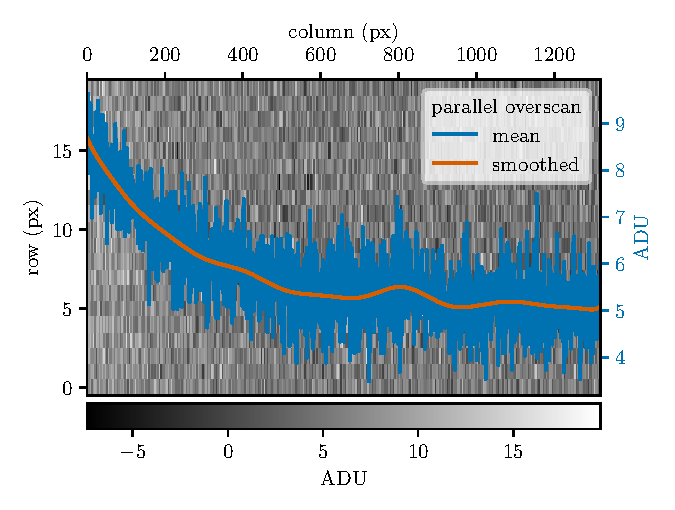
\includegraphics[width=0.65\textwidth]{figures-4/vert_oscan}
    \caption[EXPRES detector bias approximation from overscan regions]{Bias approximation using the serial and parallel overscans. The mean and subsequent smoothed mean for each overscan are shown in blue and orange, respectively. Note that the counts shown in the parallel overscan were first subtracted by the first 20 rows of the serial overscan smoothed mean, generating values close to zero.}
    \label{fig:overscan}
\end{figure}

\subsubsection{Gain}\label{gain}

The independent amplifier gains for the EXPRES CCD (Table \ref{tab:gain}) were determined empirically by matching the edges of neighboring amplifier regions based on stacked bias-subtracted extended flat images. We median combine 20 columns along each edge of two adjacent amplifier regions and determine the factor that minimizes the difference between them. We repeat this process along each row of amplifier regions, yielding a set of relative corrections for each row. Then, using the 20 median-combined rows along the center line of the detector, we determine the single factor that relates the top row of corrected amplifier regions to the bottom row.

Since these corrections are merely relative, we assume that the mean gain of the 16 amplifier regions given by the manufacturer is approximately correct. Thus, we match the mean of the empirically determined gain corrections to that given by the manufacturer. We note that the gains given by the manufacturer were not sufficient at matching the boundary conditions of the EXPRES CCD; some gain corrections were tweaked by more than 3\%.

\begin{table}[ht!]
\centering
\caption{EXPRES CCD Gain\label{tab:gain}}
    \begin{tabular}{ccc|ccc}
        \hline
        \hline
        Amplifier & Empirical & STA & Amplifier & Empirical & STA \\
        \hline
        0 & 2.57980 & 2.6645 & 8 & 2.69787 & 2.6945 \\
        1 & 2.55171 & 2.5352 & 9 & 2.65100 & 2.6422 \\
        2 & 2.53844 & 2.5218 & 10 & 2.64354 & 2.6367 \\
        3 & 2.52444 & 2.4065 & 11 & 2.60344 & 2.5502 \\
        4 & 2.51480 & 2.6024 & 12 & 2.60497 & 2.5571 \\
        5 & 2.49382 & 2.5686 & 13 & 2.59183 & 2.5630 \\
        6 & 2.52745 & 2.4816 & 14 & 2.62881 & 2.5691 \\
        7 & 2.53478 & 2.4960 & 15 & 2.72938 & 2.6111 \\
        \hline
    \end{tabular}
\end{table}

We were not able to calculate the gains in the typical manner---relating the variance of each pixel to its mean---because our flat-fielding LED source has an intrinsic variability that cannot be modeled by photon noise alone. See \citet{blackman_performance_2020} for further details.

\subsubsection{Master Extended Flat}\label{master-flat}

In order to measure the quantum efficiency (QE) variations with high signal across the relevant areas of the CCD, EXPRES employs an ``extended flat'' fiber. This rectangular fiber has slightly larger dimensions of $60 \times 180 \um$---as compared to the ``science'' rectangular fiber with dimensions $33 \times 132\um$---and is aligned with the center of the science fiber using a motor-driven mirror. Periodically throughout the operation of EXPRES, and at least once per epoch (Table \ref{tab:epochs}), the flat-fielding LED---typically used for order tracing and optimal extraction slit modeling---is injected into the extended flat fiber, and a series of more than 100 images are taken of the resultant spectrum.

Using a median combination of these extended flat images, we construct a master extended flat-field image by dividing out a smooth fit to its echellogram. For each column of each order, we fit a parametric slit function: the squared convolution of a rectangle function with a Gaussian function, which has the analytic form
\begin{equation}
    P_{x,y}(A,d,\sigma) = A \left[ \Phi \left( \frac{y+d/2}{\sqrt{2}\sigma} \right) - \Phi \left(\frac{y-d/2}{\sqrt{2}\sigma} \right) \right]^2
    \label{eq:psf}
\end{equation}
where $\Phi$ is the error function, $d$ is the width of the rectangle, $\sigma$ is the standard deviation of the Gaussian, and $A$ is the amplitude.

This choice of functional PSF form was motivated by the physical nature of EXPRES and Fourier optics approximations. The input near field of the spectrograph is a rectangle function generated by the rectangular fiber. Taking the Fourier transform of the near field yields an approximation for the far field, which is subsequently morphed as it travels along the optical path of the instrument. We approximate this morph as a Gaussian function. Therefore, the resultant near field that is captured by the detector is the inverse Fourier transform of the modified far field. Invoking the convolution theorem, this detected near field is simply the convolution of the input rectangular function with a Gaussian function, which we subsequently square to approximate the total energy of the light as it hits the detector, yielding Equation \ref{eq:psf}.

Finally, we smooth the best-fit values for $A$, $d$, and $\sigma$ along each order using a cubic spline with 10 equally spaced knots. The parameters from this smooth fit yield the profile with which we can divide the original extended flat image to generate the master extended flat-field template.

\begin{figure}
\centering
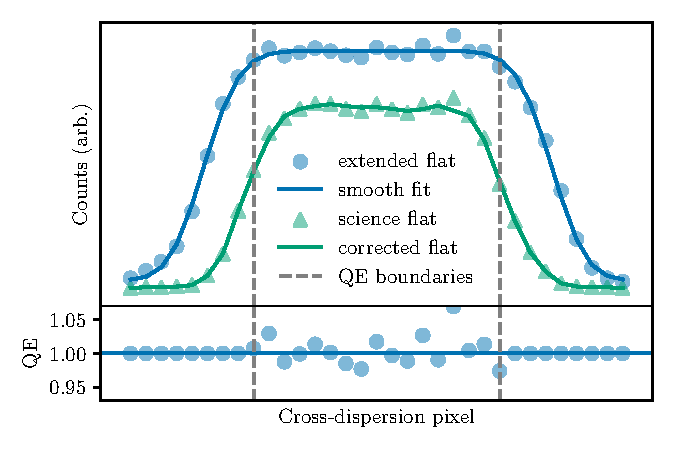
\includegraphics{figures-4/flats}
\caption[Extended flat quantum efficiency correction]{Example cross-dispersion, cross-section of an extended flat as compared to a science flat. The best fit of Equation \ref{eq:psf} is given for the extended flat. The resultant quantum efficiency (QE) corrections are shown in the lower plot and the bounds of the corrected region are demarcated. Note that these are corrections \textit{relative} to the mean QE. The QE corrected science flat is also shown in the upper plot.}\label{fig:flats}
\end{figure}

We only use pixels along the approximately flat portion of the extended slit in this constructed smooth profile. This decision was made for two reasons:
\begin{enumerate}
    \item There is less signal along the top and bottom edges of the slit, thus there is inherently more scatter in the flat corrections for these pixels.
    \item Even with the analytic function that we use, the steep edges of the slit function are difficult to fit, which leads to systematic problems in the master extended flat.
\end{enumerate}
Since the slit function of the extended flat was designed to be only 50\% larger than the science fiber slit function, the range of pixels covered by the flat portion of the extended slit (as shown in Figure \ref{fig:flats}) does not correct the entire cross-dispersion profile of the science order. Thus, we also change the motor position of the extended flat injection mirror, which moves the extended flat slit function along the cross-dispersion direction of the echellogram. We thereby expand the number of pixels included in the master extended flat by generating a master extended flat image for each mirror position and then mean-combining these images. This process is completed for each epoch.

\subsubsection{Noise Model}\label{noise-model}

The two largest contributions to the noise model for any given pixel on the EXPRES CCD are photon noise and read noise, where these two quantities are measured and summed in quadrature for each pixel. Photon noise is assumed to be Poisson, such that the standard deviation is equal to the square root of the photoelectron counts. Read noise, on the other hand, is calculated empirically for each amplifier. First, the standard deviation of the nightly stack of dark frames is determined for every bias-subtracted gain-corrected pixel. Then, the median of these standard deviations is assigned as the read noise for each amplifier region. We assume that the read noise is consistent throughout each night of observation.

For the median-combined science flat frame, there is an additional noise term: intrinsic variability in the flat-fielding LED. As described in \citet{blackman_performance_2020}, the LED brightness varies by about 0.5\% over time. The uncertainty from this variability is proportional to the counts (as opposed to photon noise, which is proportional to the square root of the counts).  Therefore, it is also summed in quadrature to produce the total noise for the science flats. As with all median- or mean-combined frames, the noise model for the science flat is divided by the square root of the number of frames.

\subsection{Spectral Extraction}\label{spectral-extraction}

``Extraction,'' in the context of the EXPRES pipeline, refers to the process of converting reduced two-dimensional CCD data into a series of one-dimensional, normalized spectra---one for each order of the echelleogram. This process involves tracing the echelle orders, removing scattered light, executing the optimal extraction, and continuum normalizing the resultant spectra. Details for these steps are found in the following sections.

\subsubsection{Order Tracing}\label{order-tracing}

The orders of the echellogram are traced using the reduced science flat frame. First, the orders are detected using a peak-finding algorithm along the mean-combined center three columns. Then, for each order, moving from this center-line outward one column at a time, triplets of neighboring columns are mean-combined and the centroid of the resultant array is calculated. The right and left ends of each order are determined by setting a S/N > 30 threshold and stopping the trace once 50 subsequent columns do not reach this threshold. Finally, these centroids are smoothed along each echelle order using a 6th degree polynomial. A single set of traces is calculated for each night of observations.

\begin{figure}
    \centering
    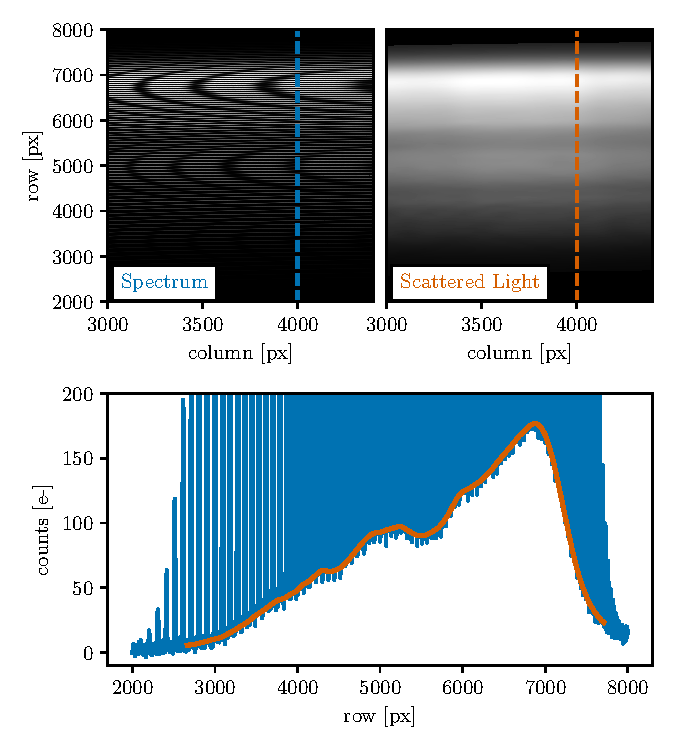
\includegraphics[width=\textwidth]{figures-4/scat_light.pdf}
    \caption[EXPRES scattered light approximation]{In the upper plot, two-dimensional scattered light approximation for reduced and median-combined science flat frames taken on 2019 October 24 are shown. The scales for the two images are not matched in order to emphasize the scattered light. The cross section of a single column (4000) for both the spectrum and calculated scattered light is shown in the lower plot. Note that the range of traced orders sets the upper and lower limits of the calculated scattered light.}
    \label{fig:scattered_light}
\end{figure}

\subsubsection{Scattered Light}\label{scattered-light}

Due to imperfections in the EXPRES optics, some scattered light from the instrument hits the CCD. This diffuse, scattered light is assumed to be smoothly varying across the detector and is estimated from the counts in the regions between the orders of the echellogram. First, a variance-weighted mean and associated uncertainty is calculated for each column of each inter-order region (including those immediately above and below the traced echellogram) using the seven pixels set halfway between adjacent traced orders. These inter-order background approximations are then smoothed using a cubic b-spline with knots set every $\sim$100 columns. Cosmic rays that could potentially skew this smoothed fit are iteratively rejected using a $5\sigma$ outlier cut.

The two-dimensional scattered light image is generated through a quadratic interpolation along each column of the smoothed inter-order backgrounds. The calculated scattered light is subtracted from the associated reduced image before any further extraction. This process is completed for the science flats, stellar frames, and all wavelength calibration frames. An example of a subregion of the resultant scattered light approximation is shown in Figure \ref{fig:scattered_light}.

\subsubsection{Optimal Extraction}\label{optimal-extraction}

\begin{figure*}
    \centering
    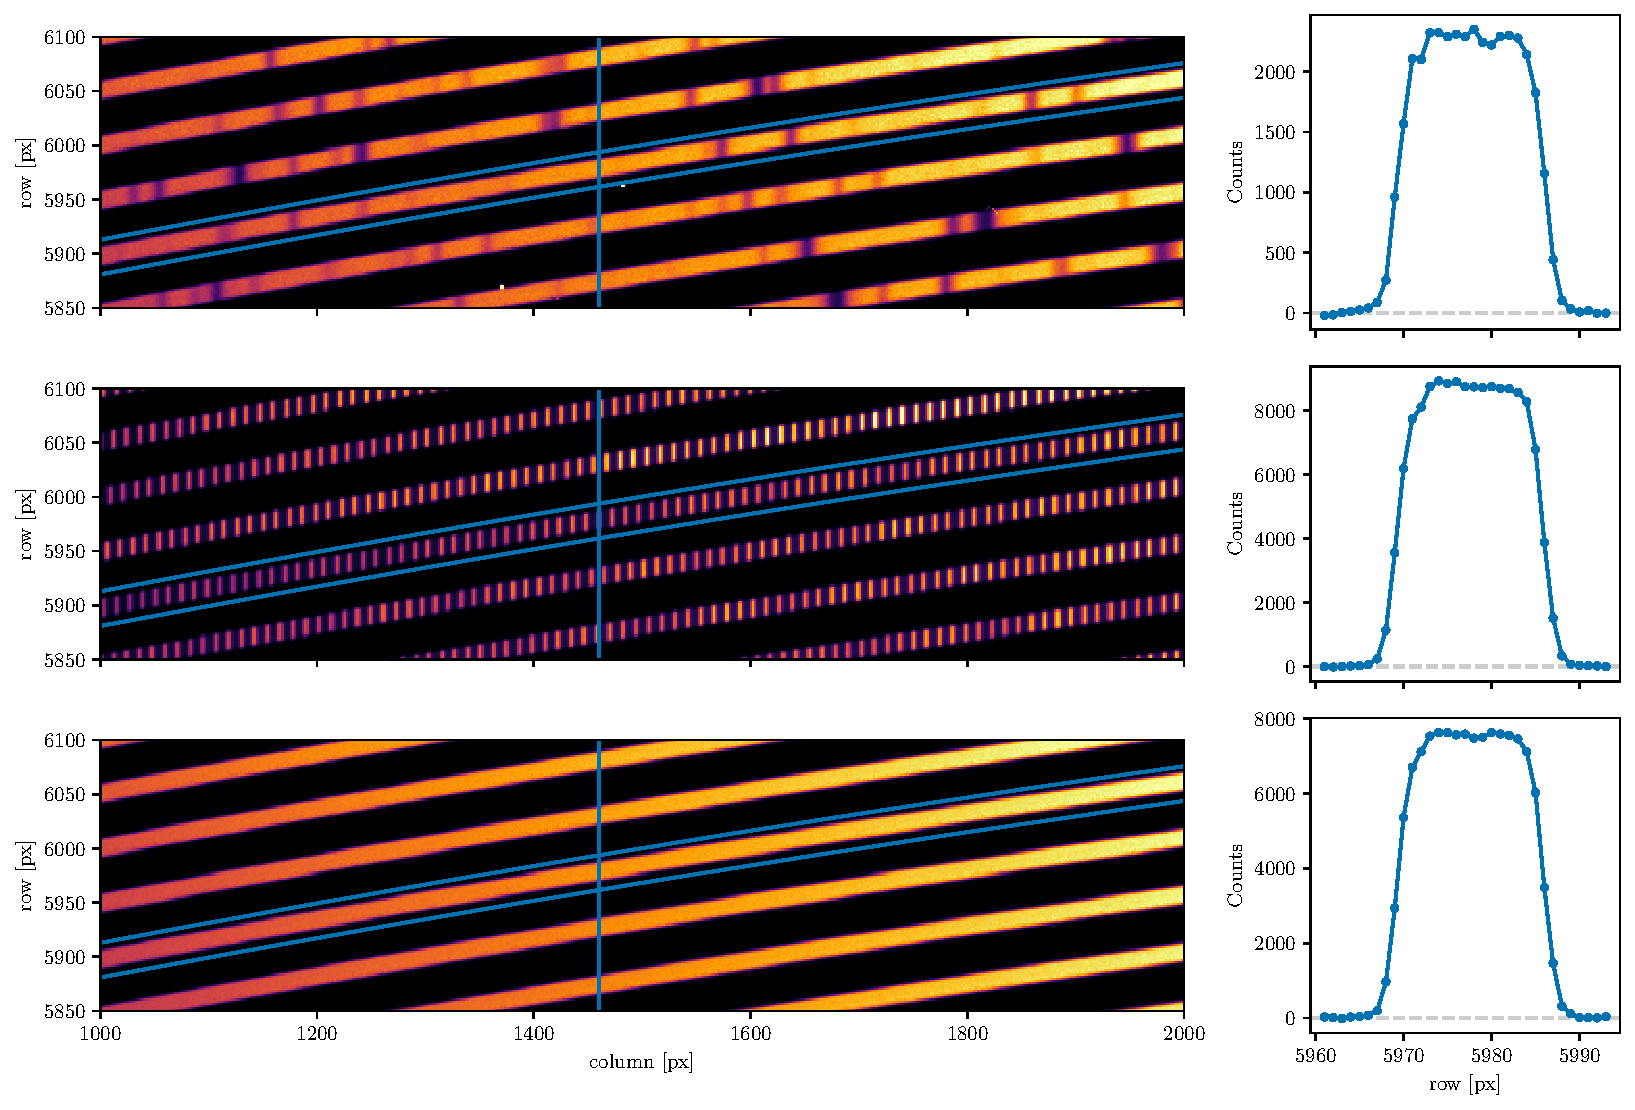
\includegraphics[width=\textwidth]{figures-4/extraction.pdf}
    \caption[EXPRES order cross-sections]{Section of raw images for a science exposure (above; HD 217014), laser frequency comb (middle), and calibration flat (below) taken with EXPRES on 24 October 2019. The extraction aperture for our optimal extraction of echelle order 100 is shown on the flat images as the intersection of the traced order (with vertical extent of 33 pixels) and the single-column slit at $x = 1460$, both shown in blue. The reduced counts in the extraction aperture for each image (i.e. removing hot pixels and QE variations) are shown in the right panels, as a function of pixel row position $y$.}
    \label{fig:extraction}
\end{figure*}

The optimal extraction algorithm that we implement in the EXPRES pipeline is an updated version of the algorithms developed by \citet{horne_optimal_1986}, \citet{piskunov_new_2002}, and \citet{zechmeister_flat-relative_2014}. Following along the traces (from Section \ref{order-tracing}) of each echelle order, we construct a least-squares estimator for each 33 pixel tall column $x$:
\begin{equation}
    \chi_x^2 = \sum_y ( D_{x,y} - P_{x,y} s_x )^2  w_{x,y}
    \label{eq:least-squares}
\end{equation}
where $D_{x,y}$ are the photoelectron counts for each pixel $(x,y)$ in the reduced data (see Figure \ref{fig:extraction}), $P_{x,y}$ is the model of the slit function corresponding to those same pixels, $s_x$ is the extracted spectral intensity, and $w_{x,y}$ are the weights for each pixel. These weights are inversely proportional to the variance of $D_{x,y}$ ($\sigma_{x,y}^2$, see Section \ref{noise-model}) and include a binary cosmic ray mask, $M_{x,y}$ (i.e. $w_{x,y} = M_{x,y} / \sigma^2_{x,y}$; see \citealt{zechmeister_flat-relative_2014}). The minimization of Equation \ref{eq:least-squares} has an analytic solution:
\begin{equation}
    s_x = \frac{\sum_y w_{x,y} D_{x,y} P_{x,y} }{\sum_y w_{x,y} P_{x,y} P_{x,y} }.
    \label{eq:least-squares-soln}
\end{equation}
The propagated uncertainty of the extraction
\begin{equation}
    \sigma_{s_x} = \sqrt{\frac{1}{\sum_y w_{x,y} P_{x,y} P_{x,y}}}
\end{equation}
is rescaled by $\chi_{\mathrm{red,}x}$ as in \citet{zechmeister_flat-relative_2014}. However, we smooth $\chi_{\mathrm{red,}x}$ across each order using a third-order polynomial before applying it to $\sigma_{s_x}$ to avoid low number statistic variance.

Cosmic rays are rejected by iteratively adding to the cosmic ray mask, $M_{x,y}$, based on a tiered outlier rejection algorithm. After calculating $s_x$ for an entire order, the residual $(D_{x,y}-P_{x,y}s_x)w_{x,y}$ for each pixel is calculated. For each column in the order with a pixel that exceeds $8\sigma$, the pixel with the largest residual is rejected and $s_x$ is re-calculated for that column. This process repeats until all $8\sigma$ outliers are rejected. Next, this same rejection process repeats for $2\sigma$ outliers that also neighbor previously rejected pixels, thus rejecting the dim tails of otherwise bright cosmic rays. Importantly, this second step is executed using two-dimensional pixel information, meaning that a bright cosmic ray on a pixel in a given column can have its tail rejected in an adjacent column.

The EXPRES pipeline has two distinct methods of approximating the model $P_{x,y}$ in Equation \ref{eq:least-squares-soln}:
\begin{enumerate}
    \item Fit each column of the science flat with a parametric slit function (Equation \ref{eq:psf}), smooth the parameters along each order using a b-spline, and then normalize the function.
    \item Use the science flat, without normalization, as in \citet{zechmeister_flat-relative_2014}.
\end{enumerate}
This yields two modes of operation when extracting data, wherein (1) keeps the echelle blaze function of each order intact while (2) intrinsically removes the blaze.

We note that using method (2) requires inclusion of the variance prior in the flat \(\sigma_{P_{x,y}}^2\), as well as that for the data \(\sigma_{D_{x,y}}^2\), when determining the weights \(w_{x,y}\) of the least-squares estimator. Therefore, the variance prior for each pixel should instead be constructed as
\begin{equation}
    \sigma^2_{x,y} = \sigma^2_{D_{x,y}} + s^2_x \sigma^2_{P_{x,y}},
\end{equation}
and an additional nonlinear cost term must be added to Equation \ref{eq:least-squares} to prevent $s_x \rightarrow \infty$. In our case, we choose \(\sum_y \ln{\sigma^2_{x,y}}\).

Thus, the minimization of Equation \ref{eq:least-squares} must be solved numerically:
\begin{equation}
    s_x^{(n+1)} = \frac{\sum_y{ w^{(n)}_{x,y} D_{x,y} P_{x,y}  }}{\sum_y{ w^{(n)}_{x,y} P_{x,y} P_{x,y}} + R^{(n)}_x}
    \label{eq:numerical-soln}
\end{equation}
where the weights $w^{(n)}_{x,y}$ for each iteration are calculated using the previous iteration's solution $s^{(n)}_x$ and $s^{(0)}_x$ is calculated assuming all $\sigma^2_{P_{x,y}} = 0$. The relaxation factor $R^{(n)}_x$ is also chosen to be
\begin{equation}
    R^{(n)}_x = \sum_y \sigma^2_{P_{x,y}} w^{(n)}_{x,y} - \sum_y \sigma^2_{P_{x,y}} \left( w^{(n)}_{x,y} \right)^2 \left( D_{x,y} - s_x^{(n)} P_{x,y} \right)^2
    \label{eq:relaxation}
\end{equation}
from the minimization of the modified Equation \ref{eq:least-squares}. This numerical process is repeated until a relative tolerance of $10^{-10}$ is met. Thus, method (2) is operationally slower than method (1), but intrinsically accounting for un-corrected QE variations and automatically removing the blaze without relying on a blaze model outweigh this minor increase in computational cost.

Removal of the blaze through method (2) can be na\"{i}vely understood by recognizing Equation \ref{eq:least-squares} is approximately solved by $s_x \approx \frac{D_{x}}{P_{x}}$, where $P_x$ is the spectral intensity of the LED source times the blaze and $D_x$ is the spectral intensity of the star times the blaze. Both $P_x$ and $D_x$ describe their respective intensity at the given column $x$ of the order. Therefore, the resultant continuum of a stellar spectrum extracted using method (2) is simply the continuum of the star divided by the spectrum of the LED source. Since both of these are slowly varying functions, we can model the extracted stellar continuum with a simple linear model for each order, calculated iteratively with $2\sigma$ outlier rejection for those pixels contained in absorption lines. See Figure \ref{fig:continuum} for examples of extracted spectra and the approximated continua.

\begin{figure}
    \centering
    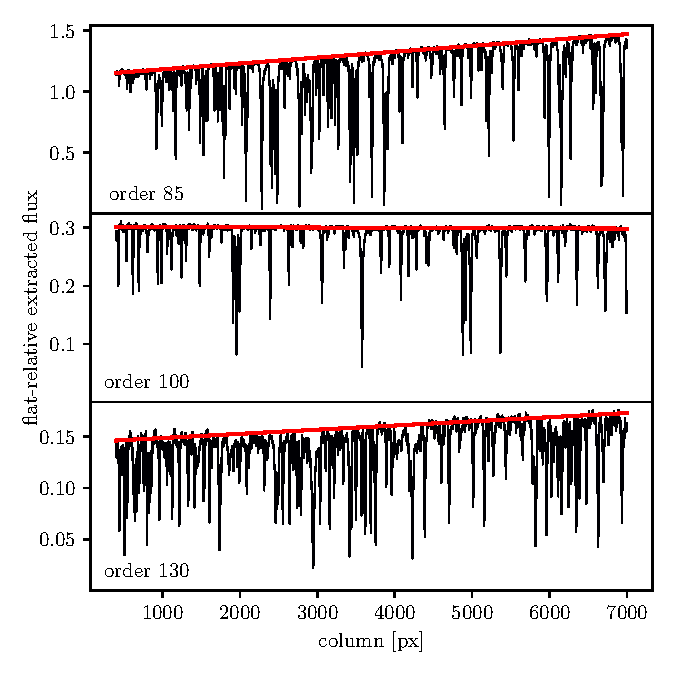
\includegraphics[width=\textwidth]{figures-4/continuum.pdf}
    \caption[EXPRES flat-relative optimale extraction and continuum normalization]{Flat-relative optimally extracted flux (black) and associated calculated continua (red) for three orders from HD 217014 observed on 2019 October 24. All continua were calculated using a linear model. Notice that the spectral flux relative to the flat-fielding LED source flux is significantly different between orders, but the resultant continuum across each order varies slowly enough to remain essentially linear.}
    \label{fig:continuum}
\end{figure}

In the EXPRES pipeline, we strictly use (2) to extract all data and only use (1) as a secondary check for our extracted RVs. However, we note that maximizing the S/N of the cross-correlation function described in Section \ref{radial-velocity-solutions} requires weights, which increase with signal-to-noise of the stellar continuum, to be assigned to different portions of the spectrum. Unfortunately, the posterior uncertainties of the extraction have too much scatter to provide these weights. We find that using the blaze function is a good proxy for a smooth weighting function; therefore, we approximate a blaze function model for each epoch using the $\alpha$-hull method \citep{xu_modeling_2019} applied to a science flat extracted with (1). We find that RV results obtained with (2), including the separately defined blaze function, are superior to those results from spectra extracted with (1).

Extraction method (2) is also the most appropriate choice for wavelength calibration spectra, such as those from the ThAr lamp and the LFC. The calibration methods used in Section \ref{wavelength-calibration} are linear and can make use of the scattered posterior uncertainties as weights when fitting each emission line without systematically shifting results as in cross-correlation. Additionally, light from the LED, ThAr lamp, and LFC all travel through approximately the same lengths of fiber, meaning removal of an instrumental response function (i.e. a calibration ``continuum'') should not be necessary when using method (2).

The S/N of a given observation is reported here as the maximum $s_x / \sigma_{s_x}$ in echelle order 111. This is effectively the per-pixel S/N at 550 nm, conforming to the metric used by \citet{fischer_state_2016} to compare many contemporaneous spectrographs. The resolution element of EXPRES contains approximately 4 pixels \citep{jurgenson_expres_2016}; thus the per-resolution-element S/N is simply twice the per-pixel S/N.

\hypertarget{wavelength-calibration}{%
\subsection{Wavelength Calibration}\label{wavelength-calibration}}

EXPRES uses a laser frequency comb (LFC) as its primary calibration source, which generates a series of spectral lines evenly spaced in frequency, whose nominal frequencies $\nu_n$ satisfy the relation
\begin{equation}
\nu_n = \nu_\text{rep} \times n + \nu_\text{offset}
\label{eq:lfc}
\end{equation}
for integers $n$. The repetition rate $\nu_\text{rep}$ and offset frequency $\nu_\text{offset}$ are referenced against a GPS-disciplined quartz oscillator, providing calibration stability corresponding to a fractional uncertainty of less than $8\times10^{-12}$ for integration times greater than 1\si{\second}.

While it is possible to obtain an absolute calibration from the LFC once the free spectral range of the echellogram has been adequately characterized, the LFC suffers from poor throughput in very blue and very red orders. In particular, although our instrumental throughput is sufficient to permit order tracing and extraction from echelle orders 75 through 160 (for $3800~\si{\angstrom}<\lambda<8220~\si{\angstrom}$), the LFC only sufficiently illuminates echelle orders 82 through 135 (for $4500~\si{\angstrom}<\lambda<7500~\si{\angstrom}$). The photonic crystal fiber (PCF) of the LFC was then replaced in 2019 July due to the decreasing stability of the LFC. With the replacement, the polarization of the LFC was switched, making the LFC redder and thus changing the orders illuminated by the LFC to echelle orders 82 through 130 (with the blue edge at 5300~\si{\angstrom}). The polarization switch should significantly increase the lifetime and stability of the LFC. Consequently, we use ThAr lamp exposures taken at the beginning and end of each night as a secondary calibration source to provide well-constrained wavelength solutions for orders outside the range of the LFC.

Calibration triplets (3 LFC's) are taken through the science fiber at roughly 15-30 minute intervals throughout observing, interwoven with science exposures. The exposure times of these calibration frames are chosen to match the target S/N of the science exposures. While EXPRES is equipped with a secondary square fiber to permit simultaneous wavelength calibrations, we choose to take calibrations through the science fiber so that our calibration data sample the same pixels and optical elements as the science exposures.  This strategy aims to homogenize our exposures to pixel-level, uncalibratable systematic errors. Also, as shown by \citet{blackman_performance_2020}, the instrumental stability of EXPRES is such that sampling the LFC every 15-30 minutes provides enough information to correct for any instrumental changes throughout the night, as simultaneous calibration would. Calibration images are taken while the telescope is slewing and so typically cost little additional time (less than 2 minutes an hour).

A ThAr wavelength solution is generated from each ThAr exposure using the IDL code \texttt{thid.pro}, developed by Jeff Valenti, which identifies ThAr lines by matching lines in an exposure against a line atlas. A sixth-order, 2D polynomial is then fitted over pixel location \(x\) and the absolute echelle order \(m\) against the scaled wavelength \(m\lambda\). Matching lines against an atlas is performed manually once at the beginning of each calibration epoch; otherwise, the wavelength solution from the immediately preceding ThAr exposure is used as an initial guess for the locations of atlas lines in a given ThAr exposure, allowing this process to be automated. Since the LFC lines are sparse relative to the precision of the ThAr calibration (1 LFC line every 10 pixels on average with the ThAr calibration accurate to the nearest pixel), this is sufficient to permit unambiguous mode identification for the LFC lines.

For any given LFC exposure, the locations of modes are identified by fitting Gaussians to each peak after a smooth background has been subtracted. An initial, trial wavelength solution is generated by linearly interpolating the ThAr solutions from the beginning and end of the night. These are used to determine the mode number \(n\) corresponding to the frequency of each mode. Once again, a 2D polynomial is fitted for \(m\lambda\) as a function of \(m\) and \(x\). Since the LFC produces a far denser set of lines (typically about 20,000 lines across 50 orders are identified in an LFC exposure, compared to about 4000 lines across 82 orders in a ThAr exposure), we use a 2D polynomial described by half of a $10\times10$ matrix of coefficients (design matrix, ninth order) for the fit. The locations of the ThAr lines are also included in the fit in order to constrain the behavior of this polynomial in echelle orders that are otherwise inaccessible to the LFC.

\begin{figure}[htbp]
    \centering
    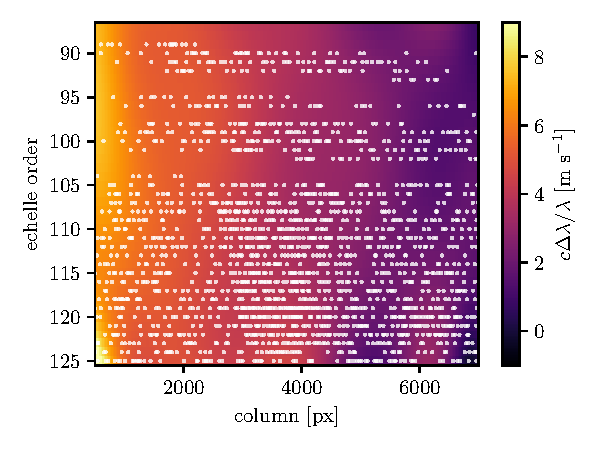
\includegraphics[width=\textwidth]{figures-4/drift.pdf}
    \caption[EXPRES wavelength calibration drift]{Calibration drift over the course of a single night (2019 October 24) for the LFC-constrained region of the echellogram, plotted in terms of the absolute echelle order number and the pixel column of the CCD. The average calibration drift for the whole night ($\sim$4.0\ms) is of similar magnitude to local variations in the drift; therefore using a single average velocity offset would necessarily incur significant additional calibration error. In other words, the wavelength solution along the left and right edges of the shown spectral format would be offset by -4.0 and +4.0\ms respectively, if a single velocity offset was used. Spectral lines used for radial-velocity solutions (shown as white dots drawn from the ESPRESSO G2 linelist) sample the detector in a nonuniform fashion and result in different overall velocity offsets, depending on spectral type.}
    \label{fig:caldrift}
\end{figure}

For each of the polynomial coefficients describing the wavelength solution, we fit a linear regression weighted by time from the middle of the observation by a Gaussian with a full-width-half-maximum of 1.5 hours. We have found that interpolating the polynomial coefficients, rather than directly interpolating the pixel-wise wavelength solutions, is more robust to imperfections in individual calibration frames. This set of 100 functions is evaluated at the photon-weighted midpoint time of each science exposure to generate a wavelength solution. This differs from the standard practice at other spectrographs (e.g. HARPS and ESPRESSO), where a single velocity offset, rather than a time-dependent wavelength solution, is assigned to each science exposure. We choose to do this in order to accommodate time-dependent variations in the characteristics of the instrument, which may lead to calibration shifts that cannot be adequately described by a single average velocity offset.

We illustrate this in Figure \ref{fig:caldrift}, where we show the calibration drift over the course of a single night in the LFC-constrained region of the echellogram. Our radial-velocity solutions (see Section \ref{radial-velocity-solutions}) sample spectral lines that are non-uniformly distributed across the detector; therefore, it is advantageous to characterize local variations to prevent overall systematic offsets. Of course, the precise differential velocity imparted by this calibration drift ultimately depends on the spectral type, as well as both barycentric and systemic velocity of the star under consideration.

As the final step in wavelength calibration, the EXPRES pipeline applies a barycentric correction to the wavelength solution of each stellar observation using the method described by \citet{blackman_accounting_2017}. For each 1~s exposure of the exposure meter, a barycentric correction is calculated using BARYCORR \citep{wright_barycentric_2014}. The photon-weighted average barycentric correction is calculated for each of eight wavelength bins of the spectra. A third-degree polynomial is then fit to these averages, yielding a smoothly varying wavelength-dependent barycentric correction \(z_\text{B}(\lambda)\) for the observation. As shown by \citet{tronsgaard_photon-weighted_2019}, it is important to distinguish this from a photon-weighted midpoint time used to calculate an overall chromatically dependent barycentric correction \citep[e.g.,][]{landoni_espresso_2014}, as this can impart a $\sim$10\cms systematic error to the radial velocity, especially in cases of longer exposure times, high airmass, or poor seeing.

Finally, we apply \(z_\text{B}\) directly to the wavelength solution:
\begin{equation}
    \lambda_\text{bary} = \lambda_\text{lab}^\text{(vac)} \left(1 + z_\text{B}\left(\lambda_\text{lab}^\text{(air)}\right)\right)
    \label{eq:bary_wavelength}
\end{equation}
where \(\lambda_\text{lab}\) is the LFC-generated lab-frame wavelength solution and \(\lambda_\text{bary}\) is the wavelength solution in the frame of the solar system barycenter. Because the EXPRES exposure meter is not in vacuum (as opposed to EXPRES itself), \(z_\text{B}(\lambda)\) is measured using air-wavelengths. Therefore, \(\lambda_\text{lab}\) is converted from vacuum to air using the algorithm and parameters derived by \citet{ciddor_refractive_1996} before applying the barycentric correction in Equation \ref{eq:bary_wavelength}.

\hypertarget{radial-velocity-solutions}{%
\subsection{Radial-velocity Solutions}\label{radial-velocity-solutions}}

The data analysis pipeline of EXPRES employs two distinct computational techniques to independently extract radial velocities from stellar spectra:
\begin{enumerate}
    \item A ``cross-correlation function'' method \citep[CCF; see][]{baranne_coravel_1979} is used to determine a rough estimate of the absolute radial velocity for each observation (Section \ref{cross-correlation}).
    \item A forward model based on a morphed NSO solar spectrum is used to derive a more precise relative radial-velocity curve (Section \ref{forward-modeling}).
\end{enumerate}
Both of these methods are currently implemented in the EXPRES pipeline for self-vali\-dation. Simultaneous results from both methods are presented in Section \ref{initial-results}. The methods as implemented in the EXPRES pipeline are described as follows.

\subsubsection{Cross-correlation}\label{cross-correlation}

As the first step in our analysis, a CCF method estimates the absolute RV of EXPRES science targets precise to several tens of \cms (depending on photon noise). We also use the CCF method to diagnose drifts and instabilities in our calibration sources, using line lists given by the comb parameters following Equation \ref{eq:lfc} for the LFC or a ThAr line atlas for the ThAr lamp.

The CCF is constructed from the input spectrum \(f(\lambda)\) as well as a spectral-type line\-list---a set of spectral lines at rest vacuum wavelengths \(\left\{\lambda_i(0)\right\}\) associated with contrast weights \(\left\{c_i\right\}\) and widths \(\left\{h_i\right\}\). For a given trial radial velocity \(v\), the wavelength of each line in the linelist is redshifted appropriately to
\begin{equation}
    \lambda_i(v) = \lambda_i(0) \sqrt{\frac{c + v}{c - v}}.
\end{equation}
The CCF is then computed as a numerical approximation to the integral
\begin{equation}
    \mathrm{CCF}(v) = \int \mathrm{d} \lambda f(\lambda) \sum_i c_i w\left(\frac{\lambda - \lambda_i(v)}{h_i}\right)
    \label{eq:ccf}
\end{equation}
where \(w\) is an arbitrary window function approximating a Dirac \(\delta\) function and \(\lambda\) is with respect to the barycentric-corrected wavelength solution from Equation \ref{eq:bary_wavelength}.

The CCF in Equation \ref{eq:ccf} is computed independently for each echelle order with a variety of trial velocities, and the CCFs for all relevant orders are co-added before a velocity model is fitted. This is a similar practice to other CCF-based RV pipelines \citep[e.g.~][]{brahm_ceres_2017}. When deriving extreme-precision radial velocities, we only include orders falling within the spectral range of the LFC, since in principle it affords considerably better sampling density and calibration stability than those regions covered by the ThAr lamp alone.

An appropriate functional model is then fitted against the co-added values of the CCF. The position parameter and posterior uncertainties of the fitted model are returned as the reported velocity and formal errors. Other quantities of astrophysical interest (e.g.,~rotational broadening width, bisector inverse slope) are also computed from the co-added CCF.

Our construction of the CCF incorporates the ability to use an arbitrary window function \(w\). In the current iteration of the EXPRES pipeline, we use a cosine function, matching other contemporary CCF implementations \citep[e.g.~][]{freudling_automated_2013, brahm_ceres_2017, modigliani_espresso_2019}. We also use a Gaussian functional model to fit the CCF for our reported radial velocities. Other possible combinations of window functions and CCF models are discussed in Section \ref{further-analysis}.


\subsubsection{Forward modeling}\label{forward-modeling}

In addition to our CCF RV solution, we have developed a new forward-modeling technique by adapting algorithms developed for the iodine RV technique \citep{marcy_precision_1992, butler_attaining_1996} as well as ideas from the ``line-by-line'' method developed by \citet{dumusque_measuring_2018}. Forward modelling from empirical stellar spectral templates is known to produce velocities with less statistical scatter than the CCF method, and typically measures relative rather than absolute radial velocities \citep{anglada-escude_harps-terra_2012}. Our modeling process is simplified relative to the iodine method because the optical design of EXPRES was optimized to provide stability in the line spread function (LSF) of the spectrograph \citep{jurgenson_expres_2016, blackman_performance_2020}, eliminating the need to model the instrumental LSF with several free parameters. In addition, free parameters for wavelength solution and dispersion are eliminated since the barycentric wavelength solution (Equation \ref{eq:bary_wavelength}) is provided as part of the nightly optimal extraction.

First, we construct a spectral template for each stellar target. An ideal template will have very high S/N and will be a good spectral match to the program stars. Our starting point is to obtain a set of four consecutive spectra---each with S/N of about 250---providing an effective S/N of 500 per pixel or S/N of 1000 per resolution element. As described by \citet{dumusque_measuring_2018}, we prefer to use spectra with low barycentric velocities so that the program spectra shift around the approximate zero-point wavelengths. The telluric contamination is then modeled in each spectrum using SELENITE \citep{leet_toward_2019} and divided out. Finally, the set of spectra are co-added.

\begin{figure}
    \centering
    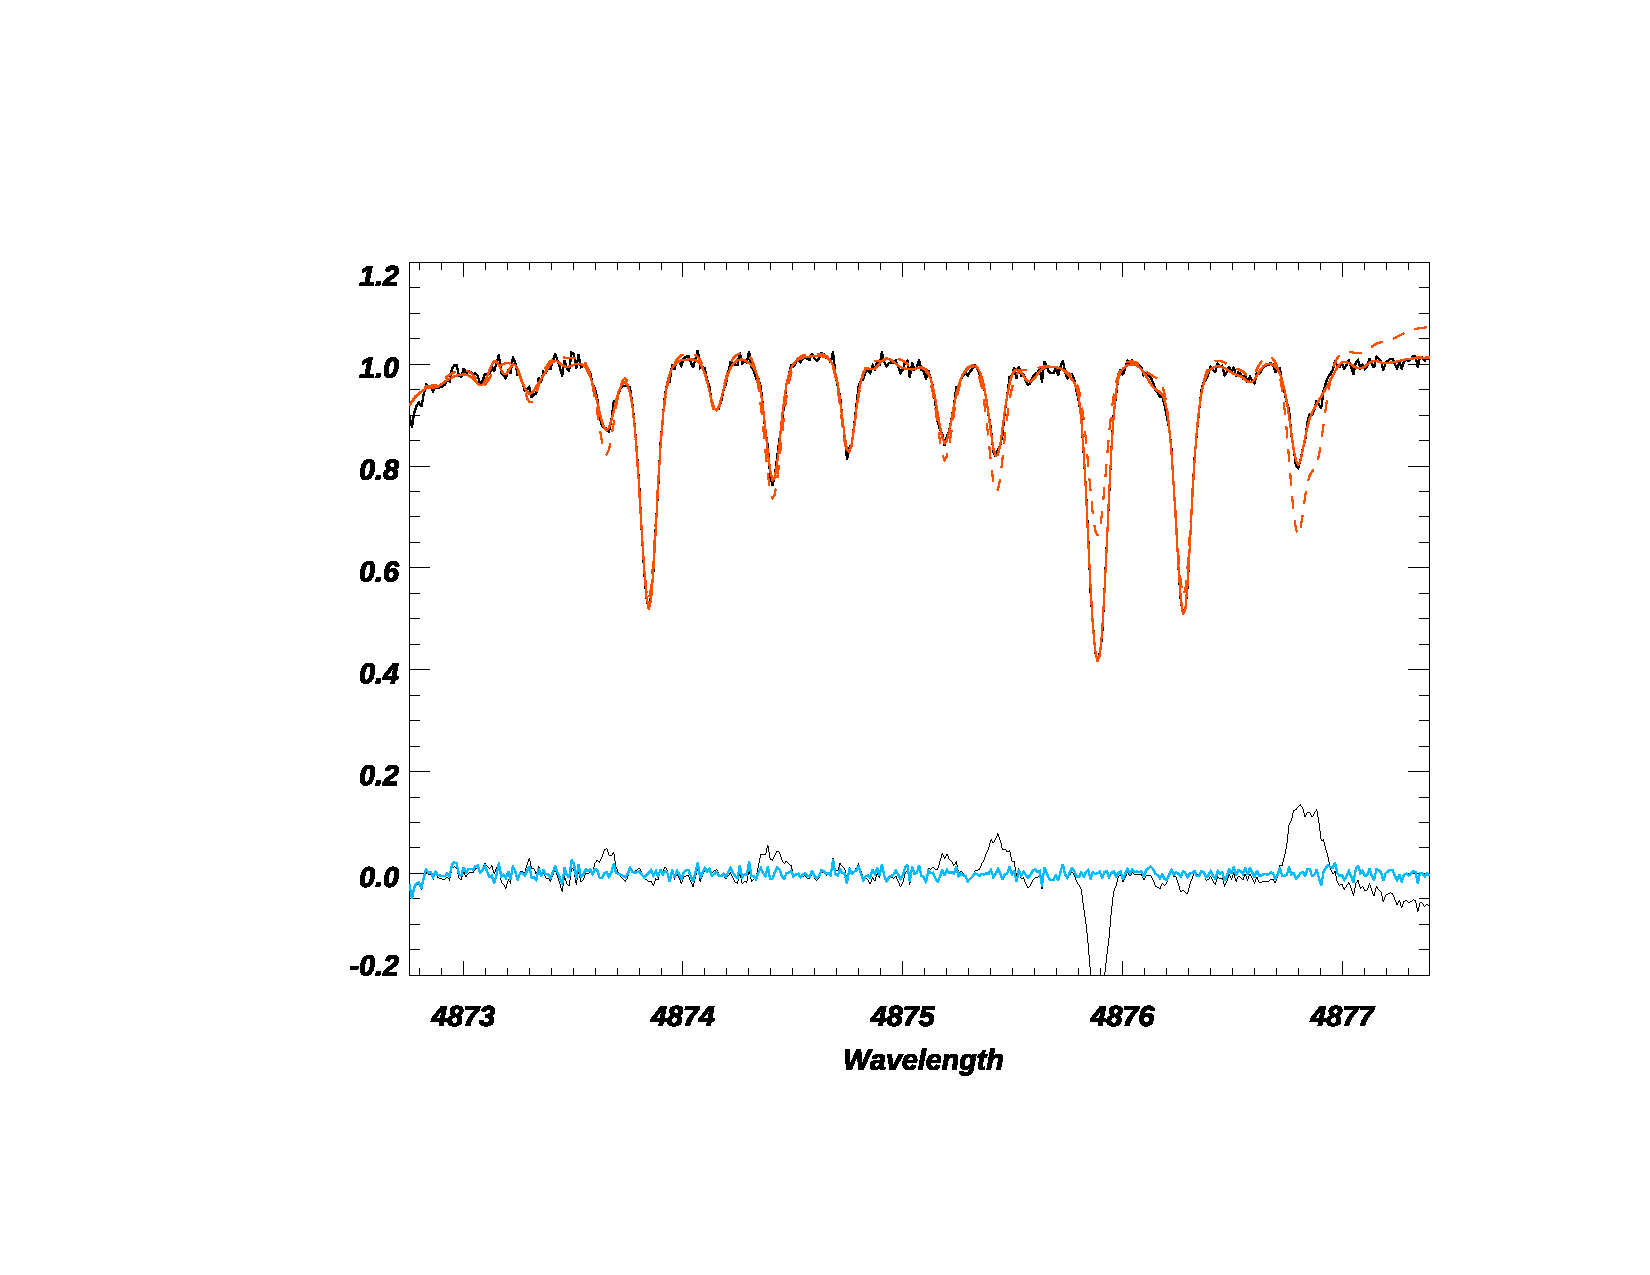
\includegraphics[trim=5cm 3cm 3cm 4cm, clip, width=\textwidth]{figures-4/morph_fit.pdf}
    \caption[NSO template for forward modeling]{High-resolution, high-S/N NSO spectrum (red dashed line) is shifted and cubic-spline interpolated to the wavelength scale of a program observation (upper black line). The difference spectrum (bottom black line) is used to identify discrepancies between the spectra above the photon-noise threshold (bottom blue line). A Levenburg--Marquardt algorithm drives the growth of pseudo-lines until the NSO spectrum has morphed to the match the spectrum of the program star (solid red line). This morphed spectrum is then used as a template for forward modeling.}
    \label{fig:morph}
\end{figure}

However, even the co-added spectrum will not provide a high enough S/N for a robust template. Therefore, we take the additional step of morphing the NSO solar spectrum (see Figure \ref{fig:morph}) with a native S/N $\sim$ 10,000 and resolution $\sim$500,000 to match the co-added, telluric-cleaned spectra for each of our program stars using the following procedure:
\begin{enumerate} 
\item The co-added program star spectrum is divided into $\sim$2000 individual chunks that are 140 pixels ($\sim $2\AA) wide within the orders of the spectrum covered by the LFC.
\item The barycentric wavelengths of the program star are used to extract a segment of the NSO spectrum with generous padding of 200 pixels for modeling shifts. This segment of the NSO spectrum is shifted to the barycentric frame of the co-added program star spectrum.
\item A Levenburg--Marquardt (L-M) least-squares algorithm is used to (i) determine the best-fit width for a Gaussian convolution kernel to rotationally broaden the NSO spectrum, (ii) refine the Doppler shift of the NSO spectrum, and (iii) apply a vertical shift to align the continuum of the NSO and the co-added spectrum. 
\item The rotationally broadened and shifted NSO spectrum is cubic-spline interpolated onto the wavelength scale of the co-added spectrum. 
\item A difference spectrum is calculated. Nodes are dropped down consecutively at points where the absolute value of the difference spectrum exceeds a threshold, characterized by the photon noise of the co-added spectrum. Pixels with the largest residuals in the difference spectrum are modeled first. The maximum number of nodes is 60, but depending on the chunk, there are typically about a dozen nodes required to model the NSO spectrum for each 130 pixel chunk. 
\item At each node, a positive or negative Gaussian feature with a width characterized by the line spread function of EXPRES is used to perturb the NSO spectrum; the depth of the morphing feature is determined by L-M fitting of the residuals. 
\item Iterative growth of the morphing lines stops when the residuals of the difference spectrum are consistent with photon noise.
\item Each chunk of the template is weighted according to the amount of spectral information, using the S/N and the derivative of intensity $I$ with pixel:
\begin{equation}
    \sum{\frac{\delta I \ \lambda}{c \ \delta \lambda} \frac{1}{\mathrm{S/N}}}
\end{equation}
\end{enumerate}

Once the template for each star has been generated, a L-M fit is executed for every 140 pixel chunk of the program star spectra. Telluric-affected pixels in each observation are assigned zero weight in the fit. There are only two free parameters for each chunk: a Doppler shift and continuum normalization scale factor. Thus, each chunk---45 LFC-calibrated orders each with about 47 chunks yielding $\sim$2000 total chunks---provides an independent measurement of the relative RV for the star. The RV for each chunk is subsequently subtracted by the mean of that chunk over all observations, thus removing any offsets that might occur because of geometric anomalies in the detector while preserving the spread in RV variations.

Weights for each chunk are determined using empirical arguments, the $\chi^2$ of the L-M fit, and a chunk-specific modifier based on its relative temporal scatter. Chunks that do not contain any absorption lines in the stellar template as well as chunks that yield relative velocities greater than $\pm$1000\ms are assigned zero weight. Moreover, chunks that have $\chi^2 > 5.0$ (typically occurring if an incorrect stellar template was used or a telluric line was missed, for example) and remaining chunks that are among those with the largest 3\% of reduced $\chi^2$ are all assigned zero weight.

Because some chunks have less spectral information, there will be more scatter in the RVs derived from these chunks. For example, chunks in the blue part of the spectrum typically have several absorption lines, but chunks in the red part of the spectrum may have only one spectral line, meaning the L-M fitting will not be well-constrained. Likewise, telluric contamination within a given chunk can manifest as large scatter in the RV over time. Therefore, the non-zero weight for given chunk $i$ within an observation $j$ is assigned as
\begin{equation}
    w_{i,j}^{-1} = \chi^2_{i,j}~\frac{\sum_{j}^{n} (v_{i,j} - \bar{v}_{j})^2}{n-1}
    \label{eq:chunk-weight}
\end{equation}
where $\bar{v}_{j}$ is the median velocity for all chunks of observation $j$ and $n$ is the total number of observations for a given stellar target. The reported RV measurement for each observation is thus a weighted mean of the individual chunk velocities, and the formal error is the corresponding standard error of the weighted mean.

\hypertarget{further-analysis}{%
\subsubsection{Further analysis}\label{further-analysis}}

Once RVs have been derived, the extracted spectra and CCFs are passed down the pipeline for more sophisticated analysis. The spectral range of EXPRES is intended to permit characterization of stellar activity and planetary atmospheric absorption lines. For chromospheric activity in particular, we extract the Ca\,\textsc{ii} line core emission ratio index $S_\mathrm{HK}$ \citep[using the parametric model of][]{isaacson_chromospheric_2010}, calibrated to yield results consistent with the Mount Wilson Observatory catalog \citep{duncan_ca_1991}.

We also aim to incorporate spectroscopic activity indicators directly into the RV solution methodology. For example, in addition to using a rectangular ``box'' function and truncated cosine in the CCF, which are implemented in other similar velocity analysis codes \citep[e.g.~][]{freudling_automated_2013, brahm_ceres_2017, modigliani_espresso_2019}, the EXPRES analysis code implements CCF computation using Gauss--Hermite window functions of the form
\begin{equation}w(x) = {1 \over \sqrt{2^n n! \sqrt{\pi}}}H_n(x) \exp\left[-{x^2 \over 2}\right],
\end{equation}
where \(H_n\) is the \textit{n}th (physicists') Hermite polynomial. Computing higher-order CCFs as coefficients in a Hermite-functional decomposition, and more generally with respect to different orthogonal basis functions, will permit more sophisticated analysis of stellar activity (via a sparse description of variations in the CCF line profile) as an alternative parameterization to current derived observables (such as the CCF bisector inverse slope/FWHM). Alternatively, data-driven decorrelation of stellar activity from bulk radial velocities, or alternative template-based RV solution methodologies \citep{holzer_hermite-gaussian_2020}, may be possible once we have built up an archive of stellar spectra.

\section{Initial Results - HD 217014}\label{initial-results}

We now present velocities derived with this pipeline based on 47 observations of HD 217014 (51 Peg) over the 10-month span between the beginning of Epoch 4 and December 1, 2019 (see Table \ref{tab:51pegvels}). We do so to examine various sources of uncertainty and error in the velocimetric pipeline, while avoiding the known instrumental instabilities inherent in Epochs 1-3 (see \citealt{blackman_performance_2020}; A. Szymkowiak et al. 2020, in preparation, for details), and to compare the two radial velocity methods outlined in Section \ref{radial-velocity-solutions}. Observations with an S/N less than 160 are not included in this analysis. We construct our CCF using the G2 line mask from the ESPRESSO pipeline \citep{freudling_automated_2013, modigliani_espresso_2019} and a cosine window function. We also fit all RVs with a single planet Keplerian model, constrained by the literature value of the orbital period \citep[4.2308 days,][]{wang_eccentricity_2011}. This Keplerian model is parameterized by the velocity semi-amplitude ($K$), the eccentricity ($e$), the argument of periastron, and a phase of periastron.

\begin{figure}[htbp]
    \centering
    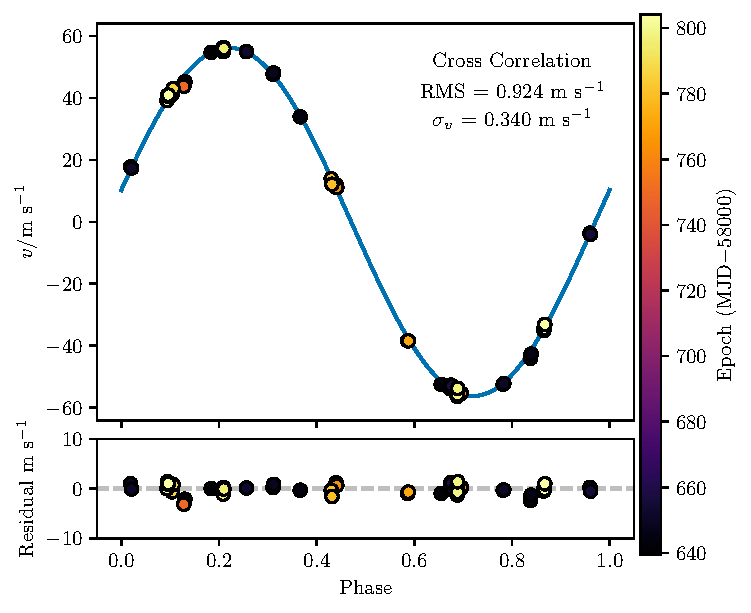
\includegraphics[width=0.8\textwidth]{figures-4/217014_ccf.pdf}
    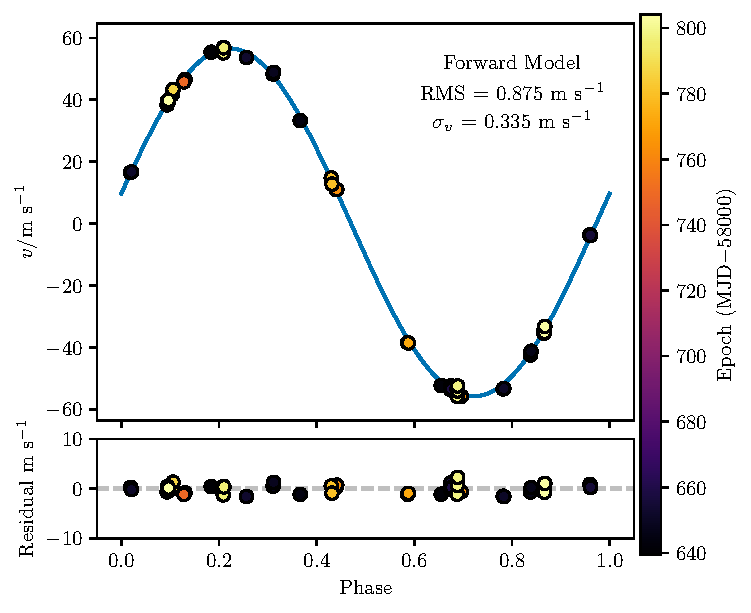
\includegraphics[width=0.8\textwidth]{figures-4/217014_cbc.pdf}
    \caption[51 Peg b -- radial velocities and Keplerian orbital fits]{Phased radial velocities, Keplerian orbital fits, and residuals for EXPRES observations of 51 Peg b. The figure is labeled with the RMS residual to the fitted orbital solution, as well as the median formal error $\sigma_v$ of all data points shown.}
    \label{fig:217014}
\end{figure}

\begin{table}[ht!]
    \centering
    \caption[51 Peg -- Commissioning radial velocities]{EXPRES commissioning RVs of 51 Peg (full data set available online)
    \label{tab:51pegvels}}
    \begin{tabular}{ccccc}
        \hline
        BMJD & $V_{ccf}/\cms$ & $V_{fm}/\cms$ & RV Epoch & S/N
        \\
        \hline
        58639.45844 & $-3320697\pm20$ & $ 5739\pm32$ & 4 & 385 \\
        58641.45174 & $-3331424\pm44$ & $-5035\pm42$ & 4 & 179 \\
        58643.46218 & $-3321644\pm34$ & $ 4854\pm34$ & 4 & 225 \\
        58644.46095 & $-3322776\pm35$ & $ 3527\pm34$ & 4 & 233 \\
        58646.45596 & $-3330577\pm39$ & $-4045\pm38$ & 4 & 203 \\
         & \(\vdots\) & & \\
        \hline
    \end{tabular}
\end{table}

Figure \ref{fig:217014} shows the resulting radial velocities from both the CCF and Forward Model methods, along with their respective orbital fits. Because the CCF uses a linelist with absolute wavelengths, the fit systemic velocity of $-33.2603(5)\unit{km\,s^{-1}}$ \citep[in excellent agreement with][]{gaia_collaboration_vizier_2018} has been removed. For each of the RV epochs, we also fit an independent velocity offset relative to the overall offset. For epochs 4 and 5, these are $-1.5(4)\ms$ and $1.2(5)\ms$ when using the CCF method, and $-1.2(8)\ms$ and $0.8(7)\ms$ when using the forward model. These offsets account for modifications to the instrumental systematics, owing to the various fiber changes and realignments. The offsets differ slightly in magnitude between the two RV analysis methods because they intrinsically weigh regions of the detector differently, accentuating or mitigating certain instrumental systematics.

\begin{table}[ht!]
\centering
\caption[51 Peg b -- Keplerian orbital fit parameters]{Fit parameters for 51 Peg b\label{tab:51peg}}
\begin{tabular}{cccccc}
\hline
Instr. & $K/\ms$ & $e$ & RMS$/\ms$ & $\sigma_v/\ms$ \\
\hline
EXPRES CCF & $56.24\pm0.14$ & $0.000\pm0.002$ & 0.924 & 0.340 \\
EXPRES FM & $56.26\pm0.13$ & $0.007\pm0.003$ & 0.875 & 0.335 \\
HARPS DRS & $53.4\pm1.6$ & $0.062\pm0.010$ & 0.941 & 1.023 \\
HIRES & $56.7\pm0.4$ & $0.020\pm0.007$ & 2.74 & 1.169 \\
%\(58271.9±0.6\)\\
\hline
\end{tabular}
\end{table}

We show the values of the Keplerian fit parameters in Table \ref{tab:51peg} along with the RMS residual and the median formal error ($\sigma_v$). The parameter uncertainties were derived by taking the square root of the product of the posterior variances and reduced $\chi^2$ of the least-squares fit. By way of comparison, we also perform the same procedure with 8 years of archival velocities from the HIRES instrument on the Keck I telescope \citep[corrected for instrumental systematics per][]{tal-or_correcting_2019} and 4 months of data from the HARPS DRS \citep{trifonov_public_2020}. The EXPRES orbital solution parameters for 51 Peg are consistent with those returned from these previous studies, but with higher precision due to the improved formal errors. The two EXPRES RV methods are also internally consistent, with the forward model producing a slightly more favorable RMS. Finally, we note that the RMS of the EXPRES fit residuals approximately matches that of the HARPS DRS, with the EXPRES fit returning parameters more comparable with literature values \citep{wang_eccentricity_2011, bedell_wobble_2019, wilson_first_2019}. 


\hypertarget{discussion}{%
\section{Discussion}\label{discussion}}

Each step of the pipeline contains several free parameters---for instance, the degree of the fitting polynomials to use for the spatial wavelength solution fits and temporal smoothing, as well as various S/N thresholds for calibration line identification and order inclusion in the CCF.  To assist community users of the instrument, we have opted, as far as possible, to preselect reasonable default values for most of these parameters, which may be overridden at runtime. In what follows, we document some nonobvious but critical aspects of these systematics, and we illustrate some aspects of the decision-making process for choosing our default values for some of these parameters.

\hypertarget{formal-errors}{%
\subsection{Formal vs. true velocity errors}\label{formal-errors}}

Since the formal velocity errors returned from the CCF fitting procedure are constructed only from the co-added CCFs and their propagated errors, they do not account for effects like wavelength calibration error (inducing spurious velocity shifts) or time estimation error (via erroneous barycentric corrections). Instead, they mostly reflect velocity estimation error due to photon noise being propagated to the CCF.

On the other hand, the formal velocity errors returned from the forward model fitting procedure does include some information
about relative uncertainty in certain regions of the EXPRES detector. For instance, a chunk that tends to have a telluric line will naturally incur more spread in the measured RV for that chunk. Therefore, even though this chunk is down-weighted by our analysis, its spurious effect still propagates to the RV error.

These assumptions are borne out in Figure \ref{fig:snr}, showing these formal errors as a function of the observation S/Ns. The CCF points depend essentially only on photon noise and potentially CCD readout and optimal extraction systematics---which we are confident of having adequately accounted for---up to some constant that may depend on, for example, the choice of CCF line mask or window function, or intrinsic astrophysical properties of the target. Conversely, the Forward Model formal errors contain much more scatter, which we believe folds in some uncertainty from telluric contamination and, potentially, stellar noise. Thus, our estimation of the true photon-noise limit of EXPRES is better described by the propagated errors of the CCF analysis, though the two analyses yield quite similar results. As shown in Figure \ref{fig:snr}, we define this limit to be $30\cms$ for a single observation at the EXPRES target S/N of 250.

\begin{figure}
    \centering
    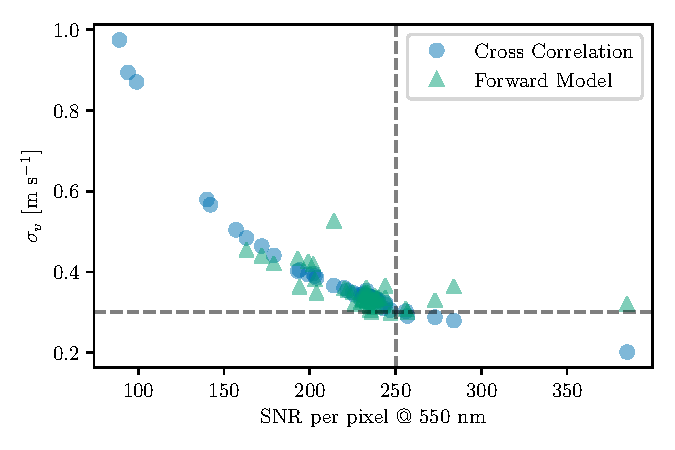
\includegraphics[width=\textwidth]{figures-4/err_vs_snr.pdf}
    \caption[EXPRES formal radial velocity errors]{Formal RV errors returned from both RV fitting procedures, plotted against the per-pixel S/N (as a characterization of photon noise) for velocities from Section \ref{initial-results}. EXPRES's target S/N of 250 is shown with a vertical line and the approximate associated formal error of 30\cms is shown with a horizontal line. Note that data here with S/N less than 160 are not included in Figure \ref{fig:217014}.}
    \label{fig:snr}
\end{figure}

Following our diagnosis and repair of the LFC beat frequency noted in Table \ref{tab:epochs}, we measured the remaining uncalibratable velocity errors arising from wavelength calibration in particular to be relatively small---between 4 and 6\cms{} RMS (A. Szymkowiak et al. 2020, in preperation). There also exist several other sources of error (e.g. from uncalibratable instrumental systematics and guiding errors) that constitute additional contributions to the RV error budget. To correctly estimate the velocimetric error, one needs to appropriately account for and then combine these error terms (e.g. by adding them in quadrature) with the formal value reported from the RV analysis. A detailed inventory of these error sources \citep{blackman_performance_2020} estimates the combined instrumental and guiding errors of EXPRES at $\sim$10\cms. Thus the single observation error of EXPRES is clearly dominated by the apparent photon noise.

\hypertarget{ccf-order-selection}{%
\subsection{Chromatic dependences}\label{ccf-order-selection}}

Many of the novel techniques that we have adopted in the EXPRES pipeline involve the introduction of chromatic dependences into quantities that have previously been considered to be uniform with wavelength, such as calibration offsets and the barycentric offset velocity. It therefore behooves us to investigate possible chromatic effects that emerge at the end of the CCF velocity-solving and orbit-fitting procedure.

The CCF analysis in Section \ref{initial-results} was performed by co-adding CCFs derived from echelle orders 126 through 86 ($4850~\si{\angstrom}<\lambda<7150~\si{\angstrom}$) before fitting an absorption-line model to derive a velocity. These orders are those for which at least $N_\mathrm{min}=19$ LFC lines are detected that pass both the S/N threshold and all quality checks imposed by our peakfitter. ($N_\mathrm{min}$ depends on the degree of the polynomial fitted to the wavelength solution, which is a free parameter in our code, as are the threshold values for these quality checks).

In Figure \ref{fig:orders}, we show the RMS residuals from the orbital solutions that arise when we repeat these analyses while varying the range of echelle orders used when co-adding CCFs; our default parameter selections are indicated with the red dotted lines. In particular, this means extrapolating the wavelength solution and chromatic barycentric correction beyond the spectral range of the LFC, which covers echelle orders 130 through 82, and of the chromatic exposure meter, which covers orders 135 through 86 ($\sim4650~\si{\angstrom}<\lambda<7150~\si{\angstrom}$).

\begin{figure}
\centering
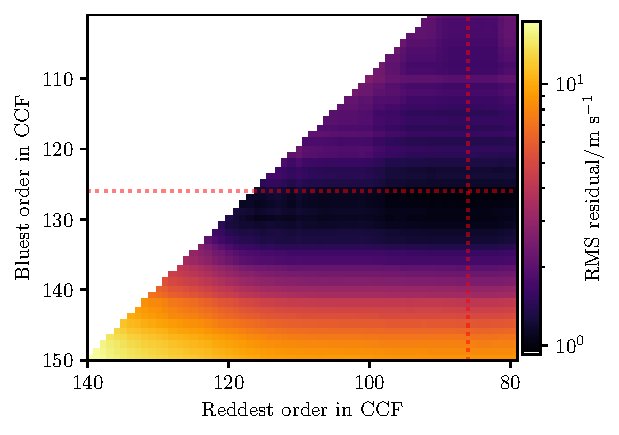
\includegraphics[width=\textwidth]{figures-4/vel_orders_217014.pdf}
\caption[Cross-correlation order range optimization]{RMS scatter from orbital solutions fitted to HD 217014 as a function of bluest and reddest echelle order included in the CCF computation. Points along each diagonal indicate sets of velocities computed with the same number of echelle orders. At least 10 echelle orders have been included in all CCF computations. Dotted red lines show the default parameters used in the preceding sections.\label{fig:orders}}
\end{figure}

For this data set, we see that there is a sharp dependence on the bluest order co-added into the CCF. Moreover, we see that the introduction of orders redder than the LFC cutoff also slightly increases the RMS error to the fit. Recalling that the wavelength solution outside of the LFC region is largely constrained by the ThAr lamp, this potentially implies a calibration offset between the LFC and the ThAr lamp, despite both sources illuminating the instrument through the same fiber.

On the other hand, we do not see any similarly sharp cutoff when extrapolating the chromatic barycentric correction to outside of the wavelength range covered by the exposure meter. This suggests that the wavelength dependences of our barycentric corrections (detailed more fully in \citealt{blackman_measured_2019}) are generally smooth enough for robust extrapolation.

Finally, it is possible to choose narrower ranges of echelle orders that yield smaller RMS errors than our default parameter selection. However, we note that this is potentially dependent on the specifics of the CCF line lists used in the computation and also possibly on underlying astrophysical properties of the science targets and other fortuitous factors. We have opted to include as many orders as can be accurate, so as to minimize photon noise, while still leaving the option to include fewer orders available to end users.


\hypertarget{conclusion}{%
\section{Conclusion}\label{conclusion}}

The commissioning process on the EXPRES instrument is essentially complete, along with the development of an optimal extraction pipeline that we have been using for preliminary RV analysis through both CCF and forward modeling techniques. Within the instrumental back-end (i.e. limiting ourselves to the calibration unit and the spectrograph proper), we have determined our photon-noise-limited RV errors to be approximately 0.3\ms for a single observation with S/N of 250. With EXPRES's current observing strategy of four observations per night per target, this result implies a nightly measurement error of only 0.15\ms. While our on-star measurement error appears to be $\sim$0.9\ms---based on residual RMS to an orbital fit of 51 Peg b---we must also note that our RV analysis pipeline does not fully address photospheric velocity sources, telluric contamination, or longer-term instrumental errors. These other sources of RV scatter are beyond the scope of this paper, although we are actively investigating them. The RV precision presented in this paper, therefore, represents our worst-case scenario in the absence of further improvements. We anticipate upcoming hardware improvements and more sophisticated RV solution methodologies to only enhance our measurement precision and long-term instrumental stability. 

Moreover, there are multiple parts of the pipeline that remain under active development. We are investigating the use of spectro-perfectionism \citep{bolton_spectro-perfectionism_2009, cornachione_full_2019} as an alternative to optimal extraction. We are also exploring a hierarchical, non-parametric wavelength solution that takes advantage of the low degrees of freedom allowed in a stabilized instrument and the density of lines offered by new wavelength calibrators \citep{zhao_excalibur_2020}. There are also plans to implement a more data-driven approach \citep[as in][with modifications to permit chromatic barycentric corrections]{bedell_wobble_2019} as yet a third RV analysis technique. 

These caveats notwithstanding, we have demonstrated that the technical innovations that have been invested into the development of novel instrumentation and software analysis techniques for EXPRES have largely paid off---they have permitted us to unambiguously attain sub-\ms on-sky radial-velocity precision. Presently, this makes EXPRES the most precise EPRV spectrograph in the Northern Hemisphere.

Finally, we hope the lessons we have learned in the process of commissioning this instrument, and the techniques we have developed, to be of some value to the community of EPRV instrument builders moving forward.

We thank the anonymous referee for comments that significantly improved this paper. We gratefully acknowledge Yale University, the Heising-Simons Foundation, and an anonymous Yale alumni donor for providing telescope time for EXPRES used to obtain the data in this paper. We also acknowledge the extensive work that went into the RePack spectral extraction code, written by Lars Buchhave; this code helped benchmark the EXPRES optimal extraction described in this paper. J.O. thanks X. Dumusque for illuminating and productive discussions. We especially thank the NSF for funding that allowed for precise wavelength calibration and software pipelines through NSF ATI-1509436 and NSF AST-1616086 and for the construction of EXPRES through MRI-1429365. This material is based on work supported by the National Science Foundation Graduate Research Fellowship under grant No. DGE1122492 (RRP, LLZ, ABD).


	\chapter{Advancements to the EXPRES Pipeline} \label{chapter:pipeline2}

\section{Introduction}

After the completion of the EXPRES pipeline and the presentation of initial results as described in Chapter \ref{chapter:pipeline}, there remained many possibilities for further improvement to the reliability and accuracy of the pipeline. Although the resultant RVs yield statistical precision around 30\cms that varies consistently with the measured signal-to-noise as shown in the previous chapter, residual RMS compared to fit Keplerian orbits still hover around the 1\ms level for HD 217014 \citep{petersburg_extreme-precision_2020} and 58\cms level for HD 3651 \citep{brewer_expres_2020}. Naturally, these levels of precision set a new standard for RV measurement in the community, but they still do not reach the expected instrumental precision determined by \citet{blackman_performance_2020} of 30\cms. Thus, I expected that improvements could nevertheless be made to the pipeline in order to push this standard even further.

In this chapter, I detail contributions I made to the pipeline beyond what was presented in the previous chapter in three separate areas. The first (Chapter \ref{pipeline2:spec-perf}) is the introduction of spectro-perfectionism to the pipeline as a step into an extra dimension of analysis as compared to optimal extraction. The second (Chapter \ref{pipeline2:bspline}) shows how B-Splines can and have been used in the pipeline to improve our understanding of the spectra that overlap adjacent \'{e}chelle orders. Finally, the third (Chapter \ref{pipeline2:forward-model}) demonstrates an application of \textit{B}-spline stellar templates as an empirical forward model to measure radial velocities.

\section{Spectro-perfectionism} \label{pipeline2:spec-perf}

Optimal extraction, even the flat-relative variety as presented in Chapter \ref{optimal-extraction}, unfortunately misses out on some information about the instrument and thus cannot maximally extract data. In particular, this is because optimal extraction extracts one column at a time across each order. This process assumes that each extract-able spectral ``bin'' is distributed only along each column without any information shared between adjacent columns on the detector.

Rather, \'{e}chelle spectrographs typically have a slit function that is wider than a single pixel on the detector and the function itself tends to have Gaussian-like tails that extend well beyond the brightest pixels of the projected slit. Therefore, there is inherent cross-talk along the columns of a single extracted order: the brightness in one pixel is highly correlated with the brightness in neighboring pixels. In addition, contemporary \'{e}chelle spectrographs are typically fiber-fed, meaning the resultant point-spread-function (PSF) of the instrument are sometimes non-rectangular and, even if rectangular, angled when compared to the alignment of the detector pixels.

To fully understand the possible issue with optimal extraction, consider the exaggerated example presented in Figure \ref{fig:angled-alignment} of a rectangular fiber that is 30-degrees from vertical in the reference frame of the detector. A flat field source projected through the spectrograph with this PSF configuration would be continuous, as expected from an aligned PSF. However, when taking vertical cross-sections of a stellar observation order with a deep absorption line and comparing them against this flat field calibration, as is done in optimal extraction, the shapes definitely do not match up.

[FIGURE WITH 30-DEGREE MISALIGNED FIBER AND RESULTANT FLAT]

Therefore, \citet{bolton_spectro-perfectionism_2009} devised \textit{spectro-perfectionism}, a numerical method that includes as much information about the PSF as possible during the extraction process. Simply, spectro-perfectionism attempts to deconvolve each \'{e}chelle order using knowledge of the 2D PSF at every position along the order trace, yielding an array of statistically uncorrelated spectral bins. Thus, implementation of spectro-perfectionism is two-fold:
\begin{enumerate}
    \item Determination of the PSF at any position on the detector and
    \item Execution of the deconvolution algorithm.
\end{enumerate}

In this section, I describe my own implementation of spectro-perfectionism for use in extracting EXPRES spectra. As far as I'm aware, spectro-perfectionism has only been implemented with SDSS-II \citep{bolton_spectro-perfectionism_2009} and Minerva-Red \citep{cornachione_full_2019} with results that appear comparable to those from optimal extraction. However, there are two major improvements that I present here from my work:
\begin{enumerate}
    \item The use of a ``flat-relative PSF'' and
    \item Optimizations that enable extraction of a full order simultaneously.
\end{enumerate}

A typical complaint about spectro-perfectionism is that it is limited by the ability to measure the instrument's PSF: inaccuracies in the PSF at any given position easily propagate along the order and can affect large swaths of data. Therefore, I propose using a flat-relative approach (similar to what I implemented with EXPRES's optimal extraction), which as I show in section \ref{pipeline2:spec-perf:psf} helps by reducing the dimensionality of the problem.

Also, one possible concern I had with the implementation by \citet{cornachione_full_2019} is the fact that each order is chopped up into multiple sections during deconvolution. Considering the implications of hard borders on a deconvolution problem (see e.g. the Gibbs phenomenon), it's likely this would introduce ringing artifacts into the extracted data. As I show in section \ref{pipeline2:spec-perf:sp}, extraction of a full order (even one nearly 8000 pixels wide) with spectro-perfectionism is computationally tractable and mitigates possible artifacting.


\subsection{The Deconvolution Problem} \label{pipeline2:spec-perf:bkgd}

In principle, \'{e}chelle spectrograph extraction is a convolution problem. The reduced (see Chapter \ref{reduction}) detector data $D_{x,y}$ with pixel indices $(x, y)$ for a given \'{e}chelle order is a convolution of the spectral intensities ($s(\lambda)$ at wavelength $\gamma$) and the instrument's wavelength-dependent PSF $\Psi_{x,y}(\lambda)$ with added photon- and read-noise $n_{x,y}$:
\begin{equation}
    D_{x,y} = \int \Psi_{x,y}(\lambda) s(\lambda) \dd{\lambda} + n_{x,y}.
\end{equation}
\label{eq:convolution-integral}
Since the orders on the EXPRES spectrograph are spaced relatively far apart, I assume they are functionally independent in this framework. Extraction is therefore solving for $s(\lambda)$ given $D_{x,y}$ and some knowledge of $\Psi_{x,y}(\lambda)$.

In order to make Equation \ref{eq:convolution-integral} numerically solvable, it must be discretized such that $\vb{s}$ is a vector at given wavelength sampling positions {$\lambda_x$} (the $x$ here does imply that these positions relate to pixel positions, as discussed in the next section) and $\vb{\Psi}$ is a matrix with a PSF representation at each $\lambda_x$:
\begin{equation}
    D_{x,y} = \left( \sum_\lambda \Psi_{x,y,\lambda} s_\lambda \right) + n_{x,y}
    \label{eq:convolution-index}
\end{equation}
or in matrix notation
\begin{equation}
    \vb{D} = \vb{\Psi}\vb{s} + \vb{n}
    \label{eq:convolution-matrix}
\end{equation}
Note that $\Psi_{x,y}$ at any given $\lambda$ is an extremely sparse matrix, since the PSF of the instrument is much smaller than the full detector.

Solving Equation \ref{eq:convolution-matrix} is now just a matter of $\chi^2$-minimization, which is trivially
\begin{equation}
    \vb{s} = (\vb{\Psi}^\mathrm{T} \vb{\Sigma}_{\vb{D}}^{-1/2} \vb{\Psi})^{-1} \vb{\Psi}^\mathrm{T} \vb{\Sigma}_{\vb{D}}^{-1/2} \vb{D}
    \label{eq:convolution-soln}
\end{equation}
where $\vb{\Sigma_D}$ is covariance matrix for the reduced data. I assume here that $\Sigma_D$ is diagonal (in the three-dimensional sense) because the dominant detector noise properties---particularly photon- and read-noise---are uncorrelated. That being said, off-axis terms---due to e.g. pixel non-uniformity---could be included if so desired, though with a cost to complexity.

An important observation about Equation \ref{eq:convolution-soln} is that the matrix
\begin{equation}
    \vb{\Sigma_s} = (\vb{\Psi}^\mathrm{T} \vb{\Sigma}_{\vb{D}}^{-1/2} \vb{\Psi})^{-1}
\end{equation}
is the covariance matrix associated with the extracted spectrum. Except in the case of a PSF that is perfectly aligned to the columns of the detector (which is exactly the assumption made by optimal extraction), $\vb{\Sigma_s}$ is unfortunately not diagonal, meaning the individually extracted spectral values have statistically correlated uncertainty. This construction results in significant ``ringing'' in $\vb{s}$, rendering it highly unusable as a typical spectrum.

Therefore, I also use a \textit{reconvolution matrix} $\vb{R}$ to diagonalize the covariance matrix
\begin{equation}
    \vb{\Tilde{\Sigma}_s} = \vb{R} \vb{\Sigma_s} \vb{R}^\mathrm{T}
\end{equation}
and effectively convolve the spectrum back to its expected resolution
\begin{equation}
    \vb{\Tilde{s}} = \vb{R} \vb{s}
\end{equation}
thereby removing the ringing caused by Equation \ref{eq:convolution-soln} \citep{bolton_spectro-perfectionism_2009}. The full derivation for $\vb{R}$, which involves taking the matrix square root of $\vb{\Sigma_s}$ and normalizing each column, can be found in \citet{bolton_spectro-perfectionism_2009} in Section 3.

\subsection{Flat-relative Point Spread Function Modeling} \label{pipeline2:spec-perf:psf}

The first step in executing a spectro-perfectionism algorithm is determining the PSF of the instrument. Ideally, the PSF of a spectrograph would be constant across the entire CCD, immensely simplifying the computation costs of the deconvolution. However, the PSF of EXPRES (and most contemporaeneous spectrographs) changes significantly between orders and even along a single order. For example, the bluest orders on the EXPRES detector are about 2 pixels taller than the reddest orders. Thus, a parameterized PSF model is necessary to map out the PSF pixel-by-pixel.

As in previous iterations of spectro-perfectionism \citep{bolton_spectro-perfectionism_2009, cornachione_full_2019}, the EXPRES PSF model can be fully constructed in two dimensions. For this, I choose a extension of the one-dimensional function presented in Chapter \ref{master-flat} used for modelling the cross-dispersion shape of the extended flat. In two dimensions, this function has the analytic form
\begin{multline}
    \Psi(x, y; A, x_0, y_0, \theta_x, \theta_y, d_x, d_y, \sigma_x, \sigma_y) = \\
    \frac{A}{4} \Bigg[\Phi\bigg(\frac{x' + d_x/2}{\sigma_x \sqrt{2}}\bigg) - \Phi\bigg(\frac{x' - d_x/2}{\sigma_x \sqrt{2}}\bigg)\Bigg] \Bigg[\Phi\bigg(\frac{y' + d_y/2}{\sigma_y \sqrt{2}}\bigg) - \Phi\bigg(\frac{y' - d_y/2}{\sigma_y \sqrt{2}}\bigg)\Bigg]
    \label{eq:expres_psf}
\end{multline}
where $\Phi(x)$ is the error function, and $x',y'$ are related to $x,y$ by a linear transformation as
\begin{equation}
    \begin{bmatrix}x' \\ y' \end{bmatrix} = 
    \begin{bmatrix}\cos \theta_x & -\sin\theta_x \\ \sin \theta_y & \cos\theta_y\end{bmatrix}\begin{bmatrix}x-x_0 \\ y-y_0\end{bmatrix}.
    \label{eq:pix-transformation}
\end{equation}

This parameterization is advantageous because it is aptly descriptive of the Fourier optics approximation introduced in Chapter \ref{master-flat}:
\begin{itemize}
    \item $x_0$ and $y_0$ are the given pixel position of the parameterized PSF,
    \item $d_x$ and $d_y$ are the dimensions of the rectangular fiber input after dispersion and cross-dispersion stretching,
    \item $\sigma_x$ and $\sigma_y$ correlate with the amount of Gaussian smoothing caused by the EXPRES optics along each dimension,
    \item $\theta_x$ corresponds to the angular misalignment of the fiber input to the pixels of the detector, and
    \item $\theta_y$ corresponds to the local slope of the order trace.
\end{itemize}
Not only does this model allow us to map the PSF across the CCD with only eight parameters (and a variable amplitude), it also provides information on the magnification and de-focusing of the instrument. Also, since we expect these parameters to vary smoothly across the detector, we can more easily interpolate (and possibly extrapolate) to regions without easily measurable PSFs.

There is, however, a method to construct the PSF of EXPRES with fewer parameters and using more empiric information from the instrument. I call this a \textit{flat-relative} PSF, since it was influenced by the flat-relative optimal extraction work by \citet{zechmeister_flat-relative_2014} that was implemented within the EXPRES pipeline as in Chapter \ref{optimal-extraction}. The science flats provided nightly with EXPRES contain a wealth of information about the cross-dispersion (or $y$-direction) PSF of the instrument as well as pixel-level variations. These qualities are what provide such an excellent one-dimensional extraction model in Chapter \ref{chapter:pipeline}, therefore it follows that the nightly flats should be useful when constructing the two-dimensional model for spectro-perfectionism.

The flat-relative two-dimensional model used with EXPRES is the product of a one-dimensional Super-Gaussian with the nightly median-combined science flat:
\begin{equation}
    \Psi(x, y; A, x_0, y_0, \theta_x, d_x, p_x) = \frac{A}{b_x} \exp{-\left(\frac{x'^2}{2\sigma_x^2}\right)^{p_x}}~F(x,y)
    \label{eq:flat-relative-psf}
\end{equation}
where
\begin{equation}
    b_x = \sqrt{2}~\frac{\sigma_x}{p_x}~\Gamma\left(\frac{1}{2 p_x}\right),
\end{equation}
\begin{equation}
    \sigma_x = \frac{d_x}{2\sqrt{2 \log{2}^{1/p_x}}},
\end{equation}
$\Gamma$ is the Gamma function, $x'$ is defined as in Equation \ref{eq:pix-transformation}, and $F(x,y)$ is the nightly reduced science flat. Note the subtle changes in variable definitions using this new form:
\begin{itemize}
    \item $d_x$ is the full width half maximum of the Super-Gaussian,
    \item $p_x$ is the power of the Super-Gaussian, where a higher value here means a flatter top to the PSF,
    \item $\sigma_x$ is able to be calculated directly from $d_x$ and $p_x$, and
    \item $b_x$ is simply a normalization factor for the amplitude $A$.
\end{itemize}
The Super-Gaussian is used over the convolved rectangle due to an emergent degeneracy between $d_x$ and $\sigma_x$ at small $d_x$ when Equation \ref{eq:expres_psf} is used in only the $x$ dimension. Note the overall loss of complexity in Equation \ref{eq:flat-relative-psf}: the three unknown $y$-direction parameters are all completely replaced by known information from the science flat.

Measurement of an \'{e}chelle spectrograph PSF requires a sparse emission line source where each line has a width significantly smaller than the resolution of the instrument. In the case of EXPRES, I have used two different types of sources to characterize the PSF: (1) the AlN microcomb described in Chapter \ref{chapter:astro-comb} and (2) the nightly set of ThAr-lamp observations taken as wavelength calibrations. ThAr observations are unfortunately not ideal due to the existence of numerous line blends---two distinct emission lines that are closer than a single resolution element of the instrument---and near-continua of Thorium-Oxide contamination that exist throughout the spectrum. Therefore, with its evenly spaced resolved lines, the microcomb should yield a better single PSF parameterization. However, because of observed nightly movement of the instrument (see e.g. \citet{blackman_performance_2020} and Chapter \ref{wavelength-calibration}), the PSF does demonstrably change night-to-night. Therefore, in order to best incorporate spectro-perfectionism into the EXPRES pipeline, the nightly ThAr observations are used to measure the PSF. However, I will note that the microcomb measurements were used to visualize a possible ``ideal'' characterization and to better tune the eventual PSF models.

\begin{figure}
    \centering
    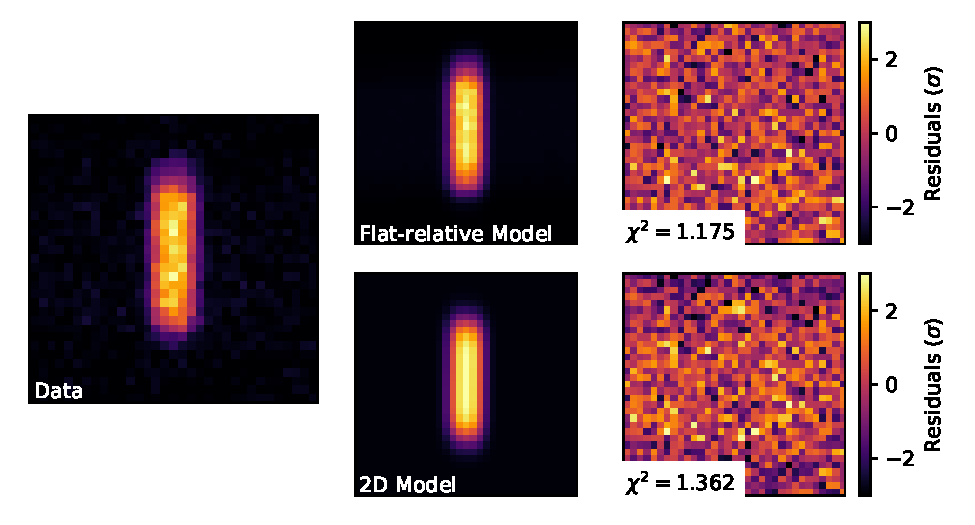
\includegraphics[width=\textwidth]{figures-5/expres-psf.pdf}
    \caption{Fit PSF model and residuals (along with corresponding $\chi^2$) using both the two-dimensional model (Equation \ref{eq:expres_psf}) and the flat-relative model (Equation \ref{eq:flat-relative-psf}).}
    \label{fig:psf-resid}
\end{figure}

In order to characterize the EXPRES PSF, I have implemented a Python sub-package within the EXPRES pipeline presented in Chapter \ref{chapter:pipeline}. This PSF sub-package uses a reduced observation of an emission line source to
\begin{enumerate}
    \item find the positions of individual emission lines, either universally or only along nightly traced orders,
    \item fit any arbitrary PSF function (including flat-relative varieties) to each emission line (see Figure \ref{fig:psf-resid}, masking severe pixel outliers (typically cosmic rays) and rejecting lines not fit well enough by the model (typically blended ThAr lines), and
    \item fit a two-dimensional polynomial (a $4 \times 4$ coefficient matrix with a Design Matrix structure as in Chapter \ref{wavelength-calibration}) to each of the PSF fit parameters, such that an interpolated PSF could be constructed for any pixel-position on the detector or for any pixel along a traced order (see Figures \ref{fig:psf-params-1d} and \ref{fig:psf-params-2d}).
\end{enumerate}
This code is relatively fast, able to map the PSF from a single image in less than two minutes using Equation \ref{eq:flat-relative-psf} and less than five minutes using Equation \ref{eq:expres_psf}.

\begin{figure}
    \centering
    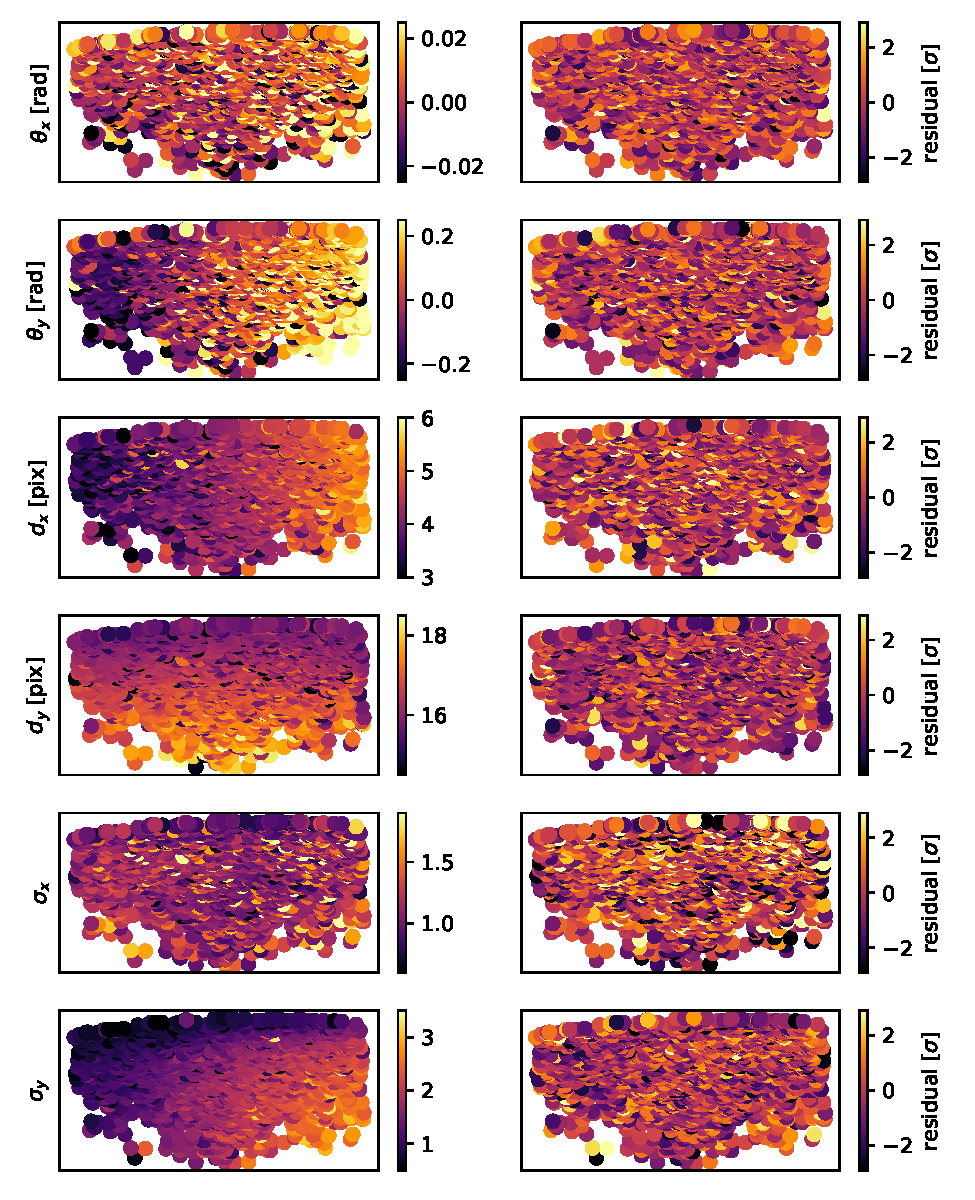
\includegraphics[width=\textwidth]{figures-5/psf-params-2d.pdf}
    \caption{PSF parameters from Equation \ref{eq:expres_psf} mapped across the detector using a ThAr observation from October 24, 2020. 1736 lines were fit using this method. Residuals from the 2D polynomial regression are presented alongside the parameters.}
    \label{fig:psf-params-2d}
\end{figure}

\begin{figure}
    \centering
    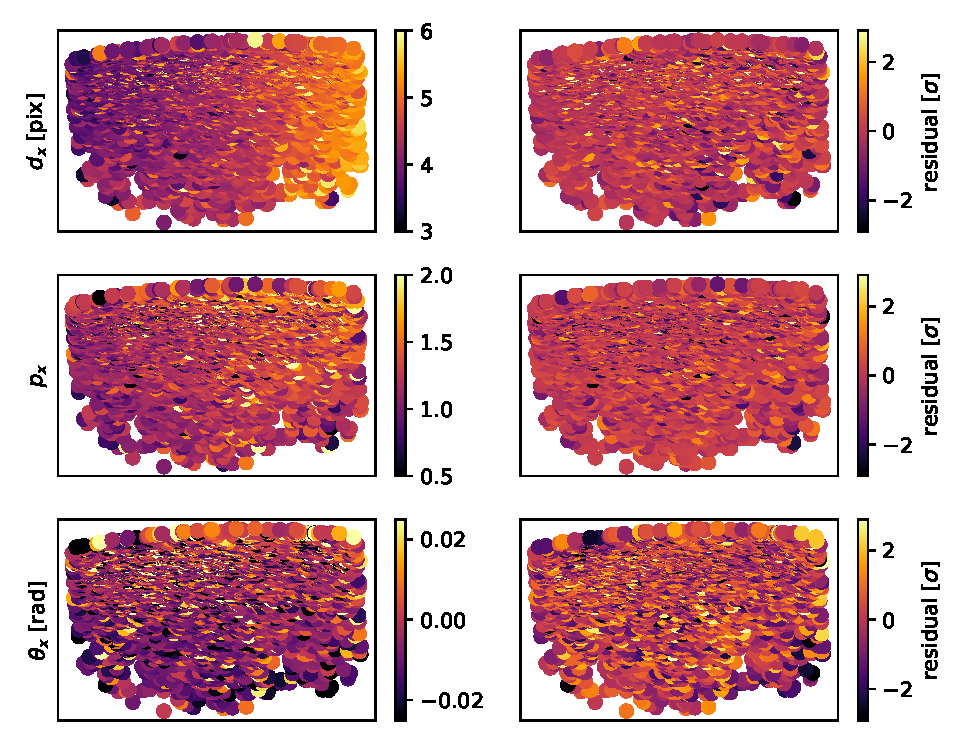
\includegraphics[width=\textwidth]{figures-5/psf-params-1d.pdf}
    \caption{PSF parameters from Equation \ref{eq:flat-relative-psf} mapped across the detector using a ThAr observation from October 24, 2020. 4367 lines were fit using this method. Residuals from the 2D polynomial regression are presented alongside the parameters.}
    \label{fig:psf-params-1d}
\end{figure}

Residual images for the two-dimenstional PSF model (Figure \ref{fig:psf-params-2d}) and the flat-relative model (Figure \ref{fig:psf-params-1d}) demonstrate how the parameters do vary smoothly across the detector and are accurately mapped by two-dimensional cubic polynomials with less than $3\sigma$ residuals. However, for the same ThAr observation, the flat-relative model rejected far fewer lines when fitting the model. This is likely due to degeneracies in Equation \ref{eq:expres_psf} and demonstrates the difficulty in developing a full two-dimensional PSF for an \'{e}chelle spectrograph.

Therefore, it is apparent that the flat-relative model has multiple advantages when characterizing the EXPRES PSF:
\begin{enumerate}
    \item use of the flat includes intrinsic detector structure in the model,
    \item fewer parameters means less computation time and model complexity,
    \item fewer lines are rejected during the regression, and
    \item flat-relative residuals are better.
\end{enumerate}
Thus, for the EXPRES implementation of spectro-perfectionism, I moved forward with exclusively using the flat-relative approach.

\subsection{Implementation Considerations}

With knowledge of the basic spectro-perfectionism algorithm and a method to construct a flat-relative PSF, there are still a handful of other considerations to make when implementing these methods. In this section, I address processing resources, cosmic-ray rejection, and extraction sampling as they are key to putting it all together.

The most glaring issue with spectro-perfectionism is the sheer potential size of the arrays used in the deconvolution and reconvolution. Considering $\vb{\Psi}$ is meant to capture the full-detector contribution of the PSF at every sampling point of $\vb{s}$, this would yield a $N \times M \times L$ array where $N$ and $M$ are the dimensions of the detector and $L$ is the number of sampled points along the order. For EXPRES, each of these quantities are greater than 5,000, making this one array (using all floating point values) 2--3 TB in memory, obviously not possible with modern memory modules. Therefore, knowing that the PSF dies extremely quickly not far from its central point as noted in Chapter \ref{pipeline2:spec-perf:bkgd}, the memory footprint can be decreased significantly by only storing a small thumbnail image at each sampled point. For EXPRES, I have set the dimensions of this thumbnail to $33 \times 33$ pixels, leaving sufficient room for the approximately $16 \times 4$ pixel rectangular PSF.

Another important computational consideration relates to the complexity of matrix operations used in calculating Equation \ref{eq:convolution-soln} and the reconvolution matrix $\vb{R}$. Specifically, $\vb{\Sigma_s}^{-1}$ is an $L \times L$ matrix that needs to be eigen-decomposed, enabling trivial calculation of both the inverse and matrix square root. Eigen-decomposition has $\mathcal{O}(L^3)$ complexity, unfortunately, meaning this problem does not scale very well, especially if implementing increased spectral sampling as discussed later in this section. Thankfully $\vb{\Sigma}_{\vb{s}}^{-1}$ is symmetric and band-diagonal which enables some sparse-matrix speed-ups.

Similar to the PSF mapping algorithms, the EXPRES implementation of spectro-perfectionism is written as a Python sub-package within the EXPRES pipeline. The algorithms---especially the matrix inversion and eigenvalue decomposition---are accelerated using SciPy's sparse linear algebra functions \citep{virtanen_scipy_2020}. Even so, extraction of a single order at single pixel sampling can take almost 30 seconds, meaning extraction of a complete spectrum can take upwards of 45 minutes within a single process of a modern iMac.

One possible speed up for the extraction, used by \citet{cornachione_full_2019} with Minerva-Red, is to run spectro-perfectionism on overlapping subsections of each order and then combine them after reconvolution. This can easily decrease the size of $L$ and therefore substantially increase the speed of the extraction. I would highly caution against this, however, due to ringing artifacts that can appear near the overlap points. Take, for example, Figure \ref{fig:spec-perf-ringing}, with an order extracted by spectro-perfectionism but in its entirety and in small chunks. Even though these two spectra appear very similar from a distance, looking at the normalized residuals between them, the spectra are clearly affected by this technique. Therefore, I maintain that each order of EXPRES is extracted completely by the spectro-perfectionism algorithm.

[PLOT OF SUPPRESSED RINGING ARTIFACTS]
\begin{figure}[H]
    \centering
    \includegraphics{figures-5/spec-perf-ringing.png}
    \caption{HD 3651, absolute order 60, extracted by spectro-perfectionism over the full order as well as in 1000 pixel chunks padded by 200 pixels. Ringing artifacts around the intersection points of adjacent chunks are readily apparent in the normalized residuals.}
    \label{fig:spec-perf-ringing}
\end{figure}

Cosmic ray rejection is built directly into the extraction algorithm, similar to EXPRES's implementation of optimal extraction (Chapter \ref{optimal-extraction}). After calculation of $\vb{s}$ as in Equation \ref{eq:convolution-soln}, a two-dimensional model of the order is generated and residuals for each pixel are calculated:
\begin{equation}
    r_{x,y} = \frac{D_{x,y} - \sum_\lambda{\Psi_{x,y,\lambda}s_\lambda}} {\Sigma_{x,y}^{-1/2}}.
    \label{eq:spec-perf-resid}
\end{equation}
All pixels with residuals greater than $5\sigma$ are masked from the data and the complete order is subsequently deconvolved again. In order to speed up this aspect of the pipeline, I only re-execute the deconvolution on portions of the CCD affected by cosmic ray masking in the previous iteration.

The final consideration is the choice of extraction sampling, since it also has implications for the computational complexity and the normalization of the flat-relative PSF. \textit{Sampling} in this context is simply the choice of how densely to extract a spectrum along a given order. Optimal extraction is limited to the horizontal pixel dimension of the detector: each spectral sample relates to one column of the detector. Spectro-perfectionism does not have this limitation since a 2D PSF could be centered on fractional pixels. Thus, there are many different ways in which a given order could be sampled. For simplicity in executing the algorithm and comparing it against optimal extraction as done in the following section, I will only present results here which have the same sampling density as optimal extraction: once per detector column. Arbitrary sampling densities, however, are still explorable with this implementation of spectro-perfectionism.

\subsection{Extraction Performance} \label{pipeline2:spec-perf:performance}

Using Equation \ref{eq:spec-perf-resid}, the modelling performance on a single order of the two PSF models, as well as that from optimal extraction, can be compared. This is visualized in Figure \ref{fig:extraction-residuals} for a portion of Order [FILL IN THIS NUMBER] for an observation of HD 3651 on [FILL IN THIS DATE]. Due to their ability to exactly match the cross-dispersion shape of the EXPRES PSF, flat-relative optimal extraction and flat-relative spectro-perfectionism clearly

[PLOT OF EXTRACTION RESIDUALS]

[PLOT OF EXTRACTED SIMULATED DATA, STAR AND LFC]

The ultimate test of spectro-perfectionism is its ability to accurately measure RVs. Between August 19, 2019, and September 17, 2020, EXPRES took [INSERT NUMBER] observations of HD 3651

[PLOT OF COMPARISON HD3651 RVs]

\subsection{Discussion}

There is much left to be explored and improved with spectro-perfectionism.

EXPRES has an advantage over other RV spectrographs which makes flat-relative spectro-perfectionism (and even, by extension, optimal extraction) more accurate: a rectangular fiber input. One of the largest improvements from using a flat-relative PSF---less complexity in the model---could be completely removed from a less separable PSF function. Take, for example, a circular or elliptical PSF. 

Gold deconvolution

Magain sampling

\section{B-Spline Regression} \label{pipeline2:bspline}

There are two distinct ways to think about and work with a spectrum after it has been extracted from an \'{e}chelle spectrograph and wavelength calibrated: (1) order-wise and (2) continuously. When dealing with a spectrum order-wise, each \'{e}chelle order is treated as functionally independent, essentially as if the end-user has 86 individual spectra to work with. This is the default behavior of the EXPRES Pipeline (Chapter \ref{chapter:pipeline}) for everything post-extraction: continuum normalization, telluric modelling, and RV analysis.

However, neighboring orders of EXPRES spectra actually overlap in wavelength significantly, meaning that a single continuous spectrum could be generated across the entire band-pass of the instrument. This is further enabled by the fact that flat-relative optimal extraction yields the same spectral output for a given wavelength regardless of which order it came from. To have the same output with a typical optimal extraction would require fitting and dividing out the blaze before combining orders, a potentially dubious process \citep{xu_modeling_2019}.

Combining orders in such a way helps by increasing signal-to-noise along the edges of each order, where the blaze function is dimmest. Since the light in these regions is shared between adjacent orders, it is beneficial to combine these signals in such a way to improve the overall fidelity of the spectrum. Overlapping ends of adjacent orders, however, do not have equivalent wavelengths sampling. Therefore, combining this data is not as simple as taking a weighted mean of spectral data at a given wavelength. Rather, the data would need to be resampled to a single wavelength grid \citep{anglada-escude_harps-terra_2012} or regressed with a smoothing function.

\textit{B}-splines \citep{de_boor_practical_1978, dierckx_curve_1995, eilers_flexible_1996} are powerful smoothing functions that can be applied specifically for this purpose. A \textit{B}-spline is a piece-wise polynomial function of order $n$ made up of a linear combination of $K$ knots ($k$) each defined by their own coefficient $c_k$
\begin{equation}
    F(x,{c_k}) = \sum_k {c_k B_{k,n}(x)}
\end{equation}
where $B_{k,n}$ are degree-$n$ basis functions of the \textit{B}-spline defined using the Cox-de Boor recursion formula \citep{de_boor_practical_1978}. $B$-splines are advantageous primarily because they can be expressed as a linear-least squares problem: uncertainties in the data are folded directly into the analysis and the regression can be run quickly even with a large amount of data, Also, the knots of a $B$-spline can be arbitrarily chosen, meaning that the ``sampling'' of this smoothing function can be chosen relative to the sampling of the instrument, whether that be undersampling to provide an estimate for the continuum, matching instrument sampling to combine orders, or oversampling when co-adding spectra to increase template resolution.

Within this section, I use the term \textit{resolution knots} to described \textit{B}-spline knots that are equally spaced by resolution, or that $\frac{\lambda_k}{\Delta \lambda_k}$ is held constant for each adjacent pair of knots. With some inspection, you'll notice that this simply means the logarithmic wavelengths of the knots are spaced equally. However, I choose to describe the ``resolution'' of the knots as a more intuitive way of understand how they are spaced within the spectrum. For example, $R=137,500$ knots would exactly match the resolution of EXPRES (one knot approximately every four pixels) while $R=600,000$ knots would be clearly oversampling the instrument with a knot essentially at each pixel.

In this section, I provide two use cases for $B$-spline regression within the EXPRES pipeline: continuum normalization (Chapter \ref{pipeline2:bspline:cont-norm}), which has already been implemented as default behaviour in the pipeline, and stellar templating (Chapter \ref{pipeline2:bspline:templates}) which provides options for combining orders and telluric modeling. In the following section, I describe how these stellar templates are used as a forward model to generate alternative RVs for EXPRES.

\subsection{Continuum Normalization} \label{pipeline2:bspline:cont-norm}

An important property of the flat-relative optimal extraction used in the EXPRES pipeline (Chapter \ref{optimal-extraction}) is that the extracted continuum across the entire spectrum is a continuous and smooth function. This smoothness enables the use of an order-wise linear regression in the previously described pipeline, but the continuity can be leveraged to easily enhance continuum normalization with the use of a $B$-spline regression for the entire spectrum.

To fit the continuum, I use an $R=100$ knot spacing and cubic ($n=2$) \textit{B}-spline basis functions. The same iterative technique of outlier rejection for absportion lines, now with a $-1.5\sigma$ cut-off, can be applied after each regression to slowly morph the \textit{B}-spline to the continuum of the spectrum. The resultant continuum at each step of this iterative process is shown in Figure \ref{fig:cont-norm-bspline}.

\begin{figure}[H]
    \centering
    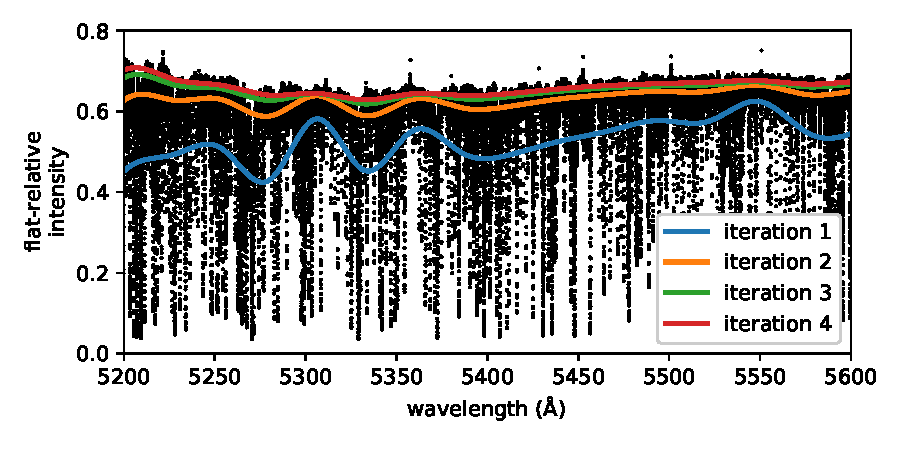
\includegraphics{figures-5/cont-norm-bspline.png}
    \caption{Iterative technique of absorption line rejection using a full-spectrum \textit{B}-spline regression. }
    \label{fig:cont-norm-bspline}
\end{figure}

The improvements with using a continuous $B$-spline regression rather than the order-wise linear fit is most apparent for \'{e}chelle orders [INSERT ORDERS HERE] where the oxygen a-band is shared between the two orders. As shown in Figure \ref{fig:cont-norm-oxygen}, the continuum in this region is certainly not perfectly linear and is better described by the local cubic function. The large gaps in the continuum are easily handled by the \textit{B}-spline as well.

\begin{figure}[H]
    \centering
    \includegraphics{figures-5/cont-norm-oxygen.png}
    \caption{Comparison of order-wise linear regression and continuous \textit{B}-spline regression for \'{e}chelle orders [INSERT ORDERS HERE] where the oxygen a-band cross between these two adjacent orders.}
    \label{fig:cont-norm-oxygen}
\end{figure}

\subsection{Stellar Templates} \label{pipeline2:bspline:templates}

This \textit{B}-spline regression can also be used to combine (or ``co-add'') multiple observations of the same stellar target together to produce a resultant template at higher signal-to-noise and resolution as compared to a single observation. As opposed to the morphed SOAP solar spectrum presented as the forward model in Chapter \ref{forward-modeling}, such a stellar template would be completely empirical and could precisely detail the nuances of both the absorption lines and the varying PSF of the instrument. No assumptions could be made about the spectra before combining them, enabling a completely data-driven approach to modeling the spectra.

Of course, multiple considerations need to be made before I can simply stack the observations on top of each other and fit them with a \textit{B}-spline:
\begin{enumerate}
    \item the spectra must be barycentric corrected to ensure they are not offset by 10's of km/s,
    \item planet-imposed stellar radial velocities could offset these spectra by 10's of m/s, and
    \item telluric contamination must be either masked or divided out in each co-added spectrum.
\end{enumerate}
Barycentric correction (1) is an inherent part of the pipeline so these large offsets are automatically corrected for. And, considering a single pixel on the EXPRES detector corresponds to approximately 500 m/s in velocity space ($R = \frac{\lambda}{\Delta\lambda} = \frac{c}{\Delta v}$), typical planetary signals (2) will not affect the data significantly enough to prevent fitting a template.

Telluric modeling, however, 

\subsection{Discussion}

The use of \textit{B}-spline regression has proven useful throughout the EXPRES pipeline. It has shown high fidelity at modeling the continuum and co-adding full spectra. There are also numerous applications to the use of these templates. For example, I am currently working on a full-spectrum telluric model code based on the order-wise algorithms developed for SELENITE \citep{leet_toward_2019}. Also, combining orders and co-adding spectra could be used to generate higher signal-to-noise indicators for stellar activity, especially in the dimmest parts of the stellar spectra around the calcium H and K lines. Finally, as I describe in the following section, co-added spetra can be used as a forward model when measuring radial velocities.

One major downside of using \textit{B}-spline regression is the lack of a simple model for posterior uncertainty. \citet{zechmeister_spectrum_2018} provide error estimates for the coefficient at each knot, which can be subsequently propagated, but these are extremely simplified and may dilute a true error analysis. Some alternatives do exist \citep{enting_propagating_2006, gardner_uncertainties_2003-1}, but their implementation are outside the scope of this work. Regardless, since the main application of the \textit{B}-spline regression in this context is as a model (for continuum, tellurics, or full spectra), the uncertainty can be assumed negligible.

An important caveat to the use of a spectrum continuously, rather than order-wise, is the fact that order-to-order spectral matching is not absolutely perfect, even when using a flat-relative optimal extraction. Since the PSF is spread across a different number of pixels on the left and right side of each order (i.e. the dispersion is not constant), there are slightly different relative contributions to a given spectral bin. An example of this is shown in Figure \ref{fig:order-matching} for a few concurrent orders of HD 3651. Note that the effect rarely produces more than $1\sigma$ residual, meaning the effect is small, but still clearly systematic. Flat-relative spectro-perfectionism could provide a solution to this issue, but it would require matching the local sampling of the PSF to the dispersion of the instrument which subsequently requires precise matching of normalization factors to each spectral bin.

\begin{figure}[H]
    \centering
    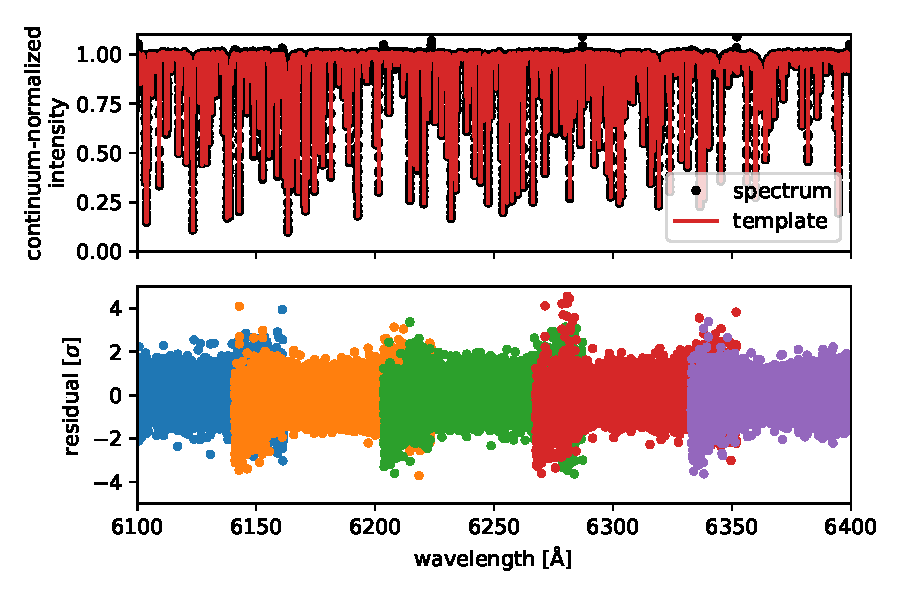
\includegraphics{figures-5/order-matching.png}
    \caption{Overlapping spectral orders of an observation of HD 3651 and the resultant residuals to the \textit{B}-spline regression. Each \'{e}chelle order is colored different to emphasize the trend. This effect is seen for all observations made with EXPRES, including wavelength calibrations.}
    \label{fig:my_label}
\end{figure}

A strong alternative to \textit{B}-spline regression could be Gaussian Process (GP) Regression \citep{rajpaul_robust_2020} due to its intrinsic ability to model uncertainty and availability of a wide variety of viable kernels to appropriately smooth the data. That being said, GPs do not scale very well, even beyond just a few hundred data points, meaning modern computational resources would not be able to come close to co-adding multiple spectra simultaneously. A spectrum from EXPRES modeled with a GP, for example, would require hundreds of separate ``chunks'' that would need to be spliced together. Thus, despite its drawbacks, I still highly recommend the use of \textit{B}-splines when combining spectral data, especially because of its speed and ability to carefully define a model resolution through knot locations.

\section{\textit{B}-spline Forward Model RV Measurement} \label{pipeline2:forward-model}

With a \textit{B}-spline stellar template in hand, I constructed a forward modeling algorithm distinct from the one presented in Chapter \ref{forward-modeling}. The primary changes within this new analysis are:
\begin{itemize}
    \item it is written in Python for simpler integration with the rest of the EXPRES pipeline,
    \item it makes use of the \textit{B}-spline stellar templates,
    \item it can optionally set the chunks to use \textit{wavelength} bins as opposed to \textit{pixel} bins.
\end{itemize}
This final point is most critical to the new implementation; since the \textit{B}-spline makes use of the full spectrum simultaneously as opposed to order-wise, it follows that the RV analysis could do the same. This enables the same benefit as for combining orders in other analysis---increased signal-to-noise along the ends of orders---which should enable greater consistency in RV measurement for these particular regions of the spectra.

The chunk-by-chunk velocity measurement is similar to that used in the IDL chunk-by-chunk analysis:
\begin{enumerate}
    \item combine all observations of the given stellar target, mask out telluric lines deeper than half the continuum and divide the given telluric model for shallower lines,
    \item use the above \textit{B}-spline regression to generate a template for the stellar target,
    \item set boundaries for chunks across the target spectrum, whether that be equal in pixels along each order (I use 100-pixel chunks) or equal in wavelength bins (I use 1~nm chunks), and
    \item run a least squares fit on each target chunk by varying the velocity offset in the wavelengths of the template, iteratively masking $5\sigma$ outliers.
\end{enumerate}
Masked residual outliers in the spectrum typically come from improper telluric modeling. An example of chunk velocities for HD 3651 are shown in Figure \ref{fig:chunk-vels} for both pixel- and wavelength-chunks.

\begin{figure}
    \centering
    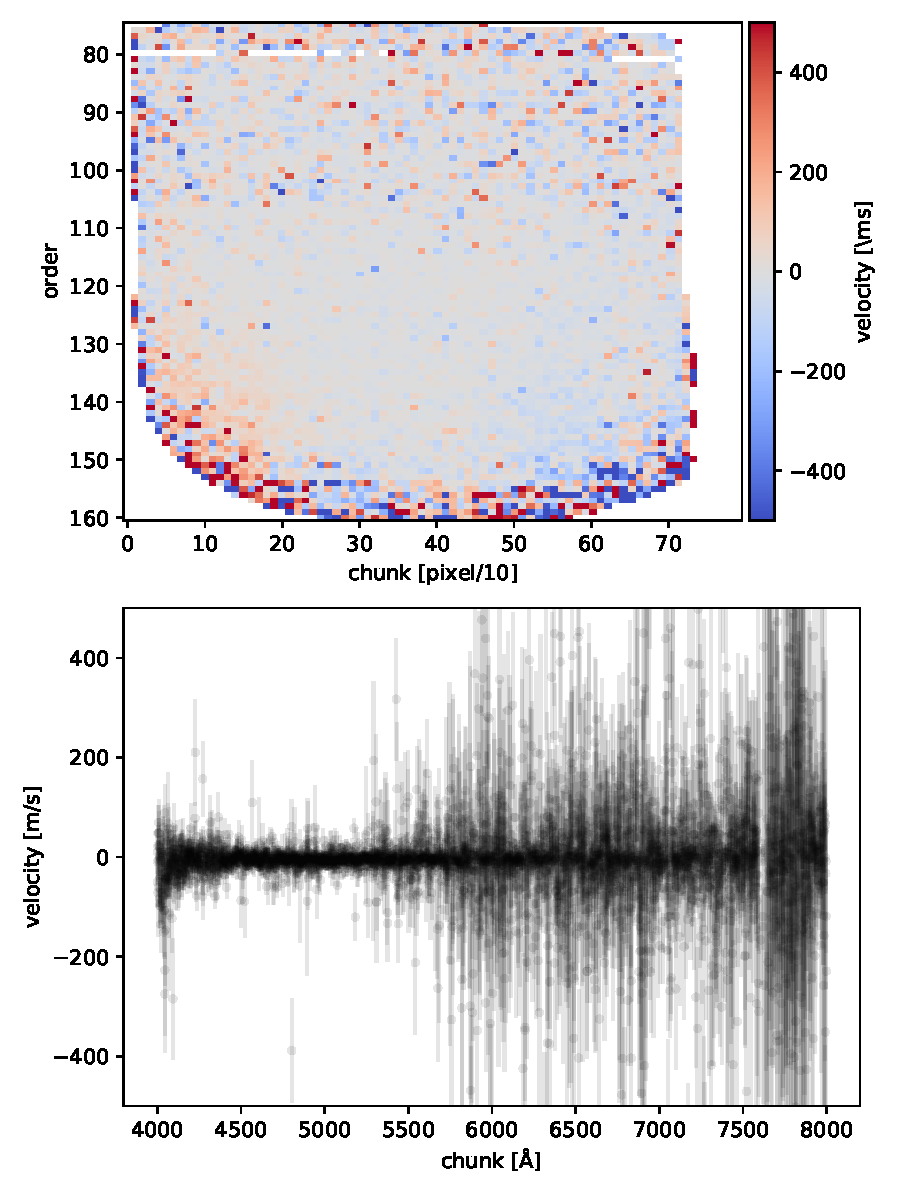
\includegraphics{figures-5/chunk-vels.pdf}
    \caption{Demonstration of chunk velocities for an observation of HD 3651 taken on October 24, 2020 using both pixel-chunks (left) and wavelength-chunks (right).}
    \label{fig:chunk-vels}
\end{figure}

Once a velocity and uncertainty is generated for each chunk, an RV for the observation can be calculated:
\begin{enumerate}
    \item calculate the variance weighted mean for each observation,
    \item calculate a variance weighted mean residual for each chunk (an approximation for the systematic velocity offset of the chunk) and subtract it from each corresponding chunk velocity of each observation,
    \item calculate a reduced $\chi$ metric for each chunk (a normalized approximation for the intrinsic velocity scatter of the chunk) and multiply it against each corresponding chunk uncertainty of each observation, and
    \item re-calculate the variance weighted mean for each observation, iteratively masking $5\sigma$ outliers one by one.
\end{enumerate}
These steps are meant to mitigate systematic effects due to the instrument (e.g. detector non-uniformities), stellar activity which may modify certain absorption lines more than others, and possible residual problems due to imperfect telluric modeling. An example of the systematic velocity offsets and reduced $\chi$ metric for each chunk is shown in Figure \ref{fig:chunk-offsets}.

\begin{figure}
    \centering
    \includegraphics{figures-5/chunk-offsets.pdf}
    \caption{Chunk mean velocity offsets (left) and reduced $\chi$ metrics (right) over all observations of HD 3651.}
    \label{fig:chunk-offsets}
\end{figure}

The data set used to compare against previous RV measurement methods is the same as used for spectro-perfectionism: observations of HD 3651 from [DATE] to [DATE]. A comparison of the velocities generated from the previous and this new forward model are shown in Figure \ref{fig:cbc-comparison} along with corresponding residuals to a Keplerian orbital fit. [ANALYSIS HERE]

\begin{figure}
    \centering
    \includegraphics{figures-5/cbc-comparison.pdf}
    \caption{Comparison of the two chunk-by-chunk velocities and corresponding residuals to a Keplerian orbital fit.}
    \label{fig:cbc-comparison}
\end{figure}


\section{Summary and Discussion} \label{pipeline2:discussion}




Huge thank you to Joel Ong for introducing me to spectro-perfectionism. I would also like to thank Adam Bolton for his conversations on this fascinatingly frustrating topic.


	\chapter{Conclusions}\label{chapter:conclusion}

In summary, this thesis presented new research to the field of radial-velocity spectroscopy instrumentation in support of various aspects of EXPRES, including its fiber architecture, wavelength calibration sources, spectral extraction, and data analysis. In Chapter \ref{chapter:modal-noise}, I found that quasi-chaotic fiber agitation, through the use of dual rotating arms, would optimally mitigate modal noise within the fibers leading to the spectrograph, decreasing laser frequency comb wavelength calibration radial-velocity scatter from 32.8~\si{\centi\meter\per\second} to 6.6~\si{\centi\meter\per\second} for EXPRES. In Chapter \ref{chapter:astro-comb}, I demonstrated the viability of aluminum nitride as a candidate for future astro-comb development, due to its high transparency and frequency conversation efficiency across a wider bandpass than that provided by the EXPRES laser frequency comb. In Chapter \ref{chapter:pipeline}, I introduced the default EXPRES flat-relative optimal extraction pipeline, yielding single measurement precision of less than 30~\si{\centi\meter\per\second} for observations with a signal-to-noise greater than 250 at 550~\si{\nano\meter} and kicking off the next-generation of radial-velocity measurement. Finally, in Chapter \ref{chapter:pipeline2}, I described further improvements made to the EXPRES pipeline---flat-relative spectro-perfectionism and \textit{B}-spline regression stellar templating---that provide radial-velocity results similar to those from the optimal extraction while also enabling greater diagnostic capability with our data.

In lieu of further summary of the conclusions already presented in the individual chapters of this thesis, I have instead organized these final conclusions into a set of lessons learned (Chapter \ref{conclusion:lessons}), a compilation of future work that could build off of this research (Chapter \ref{conclusion:future}), and my final thoughts (Chapter \ref{conclusion:final}). As a result of completing all of this work and synthesizing it into this massive document, I have been granted an extensive range of experiences that have shaped my perception of radial-velocity spectroscopy. I hope that by compiling just some of these ideas here, they can more easily be passed to those who wish to continue improving instrumentation and data extraction within this exciting field.

\section{Lessons Learned} \label{conclusion:lessons}

\textbf{Optical fiber break protection is best achieved with flexible metal sheaths}, followed by soft rubber jackets. While testing a variety of optical fibers during the modal noise study of Chapter \ref{chapter:modal-noise}, I found that fibers jacketed with hard plastic or rubber were much more likely to break than those with metal sheaths or soft rubber. This is likely due to a certain ``breaking point'' of the hard jacket, where once it is bent tighter than a certain radius, the jacket kinks and snaps the fiber. With softer or metal sheath jackets, the allowed radii of curvature are much smaller (potentially leading to worse transmission, especially in bluer wavelengths), but at least the fiber won't be broken.

\textbf{Building an in-house electro-optic modulation comb requires a high-energy pulse-width measuring device.} The greatest problem we faced while prototyping the elctro-optic modulation comb in Chapter \ref{chapter:astro-comb} was a lack of understanding the pulse width at each stage of the device. The pulse-width measurement made for Figure \ref{fig:eom-pulse} was taken with a FROG, but involved burning multiple neutral density filters due to the very high peak energy of the pulse. Investment in a more robust device early on would have certainly made this process simpler, especially since the ultimate challenge of our comb was likely insufficient pulse compression.

\textbf{Finding and fixing major outliers is more critical than incrementally tweaking algorithms.} I'll explain this using an example. Recently, in the midst of trying to improve our wavelength calibration algorithm by a few \si{\centi\meter\per\second}, we found that radial velocities from a single night were off from the rest by multiple \si{\meter\per\second}! This was caused by a failure in our interpolation scheme (a cubic polynomial fit) when less than three sets of LFCs were taken throughout the night. We fixed it by instead implementing a linear interpolation scheme with nearest neighbors weighting, decreasing velocity scatter by $\sim$1~\si{\meter\per\second} for a few target stars. Therefore, our problems were better solved by focusing on avoiding a big issue rather than tweaking small default parameters.

\textbf{Centralizing data analysis code and reporting enables quicker repairs and validation.} Data extraction and analysis for a high-resolution spectrograph is a massive enterprise. It would have not been possible to conduct much of this work by passing data from person to person in order to individually run reduction, extraction, wavelength calibration, etc. Using tools like git and features of GitHub like issue-tracking and release logs has been a life-saver, enabling better documentation and collaboration when things are going wrong. Unfortunately, one area that probably required some improvement would be central reporting of all hardware changes. With a clear record of \textit{when} the instrument was noticeably altered, we could have better correlated changes in analysis results with changes in hardware.

\section{Future Work} \label{conclusion:future}

\textbf{Further electro-optic modulation comb development.} As explained in Chapter \ref{chapter:astro-comb}, \citet{obrzud_visible_2019} used a similar electro-optic comb design to our own with some spectacular results. I believe we were on the right track with our design, but simply did not employ a long enough highly nonlinear fiber (and therefore spectral broadening) before the aluminum nitride waveguide (again, thinking big issues rather than small tweaks). Other possible areas of exploration include implementing a chirped fiber bragg grating for better dispersion control, using longer aluminum nitride waveguides, or even attempting to couple micro-rings with the electro-optic modulation comb.

\textbf{Charge Transfer Inefficiency.} One element completely missing from the EXPRES pipeline is any correction for charge transfer inefficiency \citep{goudfrooij_empirical_2006, bouchy_charge_2009, blake_impact_2017}. The mechanisms for simulating it are fairly well-known, but there has yet to be a simple pixel-wise correction model that can be applied to the reduced data. Although this effect is likely minimized on EXPRES due to consistency in signal-to-noise \citep{blackman_performance_2020}, it may play a surprisingly important (and currently uncorrected) role in laser frequency comb calibration due to the high contrast of individual comb lines.

\textbf{Telluric modeling and expanding the radial-velocity window.} I find Figure \ref{fig:chunk-vels} rather telling about where to focus radial-velocity efforts: improve telluric modeling from 550--830~\si{\nano\meter} (since the scatter here is well above 100\ms) and focus more radial-velocity analysis in the region from 400~\si{\nano\meter} to 500~\si{\nano\meter}. There is so much high fidelity data in the bluer regions of the detector and it would be a shame for us to continue not using it (another instance of thinking big!). As a first step towards better telluric modeling, I would recommend applying the \textit{B}-spline regression method of Chapter \ref{chapter:pipeline2} to the empirical analysis of B-stars from SELENITE, which currently uses simple order-wise interpolation methods. Naturally, this should be combined with continued improvements in suppressing stellar activity signals, but it seems to me that tellurics are underappreciated in our analyses.

\textbf{Spectro-perfectionism sampling study.} The biggest gain from using spectro-pefectionism over optimal extraction is its ability to sample the detector at an arbitrary rate. I would recommend implementing flat-relative spectroperfectionism such that it is normalized regardless of the sampling rate and then conducting a study to see how matching sampling to instrument dispersion may improve the fidelity of extracted spectra. In particular, I would be curious to see if overlapping orders are better aligned than when using the flat-relative optimal extraction.

\textbf{Complete spectrograph forward modeling.} According to the most recent NASA Exoplanet Exploration Analysis Program Group meeting, a high priority within the community is generating extraction code that is able to completely forward model a radial velocity into the two-dimensional pixel space of a reduced detector exposure. This would eliminate the need to move step-to-step between extraction, wavelength calibration, barycentric correction, telluric modeling, etc. where uncertainty has to be modeled and propagated through each step. Naturally, spectro-perfectionism and stellar templating may play a role in such analysis. Regardless, it will be fascinating to see if such a major shift in extraction techniques is even possible.

\section{Final thoughts} \label{conclusion:final}

The goal of discovering exoplanets that impart less than a 10~\si{\centi\meter\per\second} stellar radial velocity is certainly a lofty one. As demonstrated in this thesis, the EXtreme PREcision Spectrograph is definitely living up to its expectations of being a next-generation radial-velocity instrument. Getting to this point, however, required the expertise of multiple generations of spectrographs being passed down through their future iterations. This is how we've moved from boxcar extraction to optimal extraction to spectro-perfectionism and from iodine cells to thorium-argon lamps to mode-locked laser frequency combs to on-chip micro-ring resonators. We are absolutely within an exciting era of high-precision spectroscopy, finally leveraging the radial-velocity technique to detect Earth-like exoplanets and possibly discovering if there really is life somewhere out there.

    \addcontentsline{toc}{chapter}{Bibliography} % To get an entry in the TOC.
    \setstretch{1.0}
    
    \bibliographystyle{aasjournal}
    \bibliography{bibfile}

\end{document}
